%%%%%%%%%%%%%%%%%%%%%%%%%%%%%%%%%%%%%%%%%%%%%%%%%%%%%%%%%%%%%%%%%%%%%%%%%%%%%%
%%%%%%%%%%%%%%%%%%%%%%%%%%%%%%%%%%%%%%%%%%%%%%%%%%%%%%%%%%%%%%%%%%%%%%%%%%%%%%
%%%%%%%%%%%%%%%%%%%%%%%%%%%%%%%%%%%%%%%%%%%%%%%%%%%%%%%%%%%%%%%%%%%%%%%%%%%%%%

\chapter{Functions as Limits} \label{approx:chapter}

%%%%%%%%%%%%%%%%%%%%%%%%%%%%%%%%%%%%%%%%%%%%%%%%%%%%%%%%%%%%%%%%%%%%%%%%%%%%%%

\section{Complex numbers}
\label{sec:complexnums}

\sectionnotes{half a lecture}

\subsection{The complex plane}

In this chapter we consider approximation of functions, or in other words
functions as limits of sequences and series.
We will extend some results we already saw to a somewhat more
general setting, and we will look at some completely new results.
In particular, we consider complex-valued functions.
We gave complex numbers as examples before, but
let us start from scratch and properly define the complex number field.

A complex number is just a pair $(x,y) \in \R^2$ on which we define
multiplication (see below).
We call the set the \emph{complex numbers}\index{complex number}
and denote it by $\C$.
We identify $x \in \R$ with $(x,0) \in \C$.
The $x$-axis is then called the \emph{\myindex{real axis}} and the $y$-axis is
called the \emph{\myindex{imaginary axis}}.
As $\C$ is just the plane, we also call the set $\C$ the
\emph{\myindex{complex plane}}.

Define:
\begin{align*}
& (x,y) + (s,t) \coloneqq (x+s,y+t) , \\
& (x,y) (s,t) \coloneqq (xs-yt,xt+ys) .
\end{align*}
Under the identification above, we have $0 = (0,0)$ and $1 = (1,0)$.  These
two operations make the plane into a field (exercise).

We write a complex number $(x,y)$ as $x+iy$, where we
define\footnote{Note that engineers use $j$ instead of $i$.}
\glsadd{not:imaginary}
\begin{equation*}
i \coloneqq (0,1) .
\end{equation*}
Notice that $i^2 = (0,1)(0,1) = (0-1,0+0) = -1$.
That is, $i$ is a solution to the polynomial equation
\begin{equation*}
z^2+1=0 .
\end{equation*}
From now on, we will not use the notation $(x,y)$ and use only $x+iy$.
See \figureref{fig:complexplane}.
\begin{myfigureht}
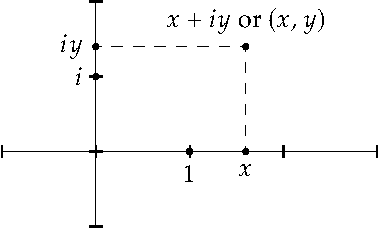
\includegraphics{figures/complexplane}
\caption{The points $1$, $i$, $x$, $iy$, and $x+iy$ in the complex
plane.\label{fig:complexplane}}
\end{myfigureht}

We generally use $x,y,r,s,t$ for real values and $z,w,\xi,\zeta$
for complex values, although that is not a hard and fast rule.  In
particular, $z$ is often used as a third real variable in $\R^3$.

\begin{defn}
Suppose $z= x+iy$.
We call $x$ 
the \emph{\myindex{real part}} of $z$, and 
we call $y$
the \emph{\myindex{imaginary part}} of $z$.  We write
\glsadd{not:realpart}\glsadd{not:imagpart}
\begin{equation*}
\Re\, z \coloneqq x , \qquad
\Im\, z \coloneqq y .
\end{equation*}
Define 
\glsadd{not:conj}
\emph{\myindex{complex conjugate}} as
\begin{equation*}
\bar{z} \coloneqq x-iy ,
\end{equation*}
and define \emph{\myindex{modulus}} as
\glsadd{not:modulus}
\begin{equation*}
\sabs{z} \coloneqq \sqrt{x^2+y^2} .
\end{equation*}
\end{defn}

Modulus is the complex analogue of the absolute value and
has similar properties.
For example,
$\sabs{zw} = \sabs{z} \, \sabs{w}$ (exercise).
The complex conjugate is a reflection of the plane across the real axis.
The real numbers are precisely those numbers for which the imaginary
part $y=0$.  In particular, they are precisely those numbers which satisfy
the equation
\begin{equation*}
z = \bar{z} .
\end{equation*}

As $\C$ is really $\R^2$, we let the metric on $\C$ be the standard
euclidean metric on $\R^2$.
In particular,
\begin{equation*}
\sabs{z} = d(z,0) , \qquad 
\text{and also} \qquad 
\sabs{z-w} = d(z,w) .
\end{equation*}
So the topology on $\C$ is
the same exact topology as the standard topology on $\R^2$
with the euclidean metric,
and $\sabs{z}$ is equal to the euclidean norm on $\R^2$.
Importantly, since $\R^2$ is a complete metric space, then
so is $\C$.
As $\sabs{z}$ is the euclidean norm on $\R^2$, we have the
\emph{triangle inequality}\index{triangle inequality!complex numbers}
of both flavors:
\begin{equation*}
\sabs{z+w} \leq \sabs{z}+\sabs{w} \qquad \text{and} \qquad
\big\lvert \sabs{z}-\sabs{w} \big\rvert \leq \sabs{z-w} .
\end{equation*}

The complex conjugate and the modulus are even more intimately related:
\begin{equation*}
\sabs{z}^2 =
x^2+y^2 =
(x+iy)(x-iy) =
z \bar{z} .
\end{equation*}

\begin{remark}
There is no natural ordering on the complex numbers.
In particular,
no ordering that makes the complex numbers into an ordered field.
Ordering is one of the things we lose when we go from real to complex
numbers.
\end{remark}

\subsection{Complex numbers and limits}

Algebraic operations with complex numbers are
continuous because convergence in 
$\R^2$ is the same as convergence for each component, and we already know
that the real algebraic operations are continuous.  For example,
write $z_n = x_n + i\,y_n$ and
$w_n = s_n + i\,t_n$, and suppose that
$\lim_{n\to\infty} z_n = z = x+i\,y$ and $\lim_{n\to\infty} w_n = w = s+i\,t$.
Let us show
\begin{equation*}
\lim_{n\to\infty} z_n w_n = zw .
\end{equation*}
First,
\begin{equation*}
z_n w_n = (x_ns_n-y_nt_n) + i(x_nt_n+y_ns_n) .
\end{equation*}
The topology on $\C$ is the same as on $\R^2$, and so
$x_n \to x$, $y_n \to y$, $s_n \to s$, and $t_n \to t$.
Hence,
\begin{equation*}
\lim_{n\to\infty} (x_ns_n-y_nt_n) = xs-yt \qquad \text{and} \qquad
\lim_{n\to\infty} (x_nt_n+y_ns_n) = xt+ys .
\end{equation*}
As
$(xs-yt)+i(xt+ys) = zw$,
\begin{equation*}
\lim_{n\to\infty} z_n w_n = zw .
\end{equation*}

Similarly the modulus and the complex conjugate are continuous functions.  We
leave the remainder of the proof of the following proposition as an exercise.

\begin{prop} \label{prop:continuityofcomplex}
Suppose $\{ z_n \}_{n=1}^\infty$, $\{ w_n \}_{n=1}^\infty$ are sequences of complex numbers converging
to $z$ and $w$ respectively.  Then
\begin{enumerate}[(i)]
\item
$\displaystyle \lim_{n\to \infty} z_n + w_n = z + w$.
\item
$\displaystyle \lim_{n\to \infty} z_n w_n = z w$.
\item
Assuming $w_n \not= 0$ for all $n$ and $w\not= 0$,
$\displaystyle \lim_{n\to \infty} \frac{z_n}{w_n} = \frac{z}{w}$.
\item
$\displaystyle \lim_{n\to \infty} \sabs{z_n} = \sabs{z}$.
\item
$\displaystyle \lim_{n\to \infty} \bar{z}_n = \bar{z}$.
\end{enumerate}
\end{prop}

As we have seen above, convergence in $\C$ is the same as convergence in
$\R^2$.  In particular, a sequence in $\C$ converges if and only if
the real and imaginary parts converge.  Therefore, feel free to apply
everything you have learned about convergence in $\R^2$, as well as
applying results about real numbers to the real and imaginary parts.

We also need convergence of complex series.  Let $\{ z_n \}_{n=1}^\infty$ be a
sequence of complex
numbers. The series
\begin{equation*}
\sum_{n=1}^\infty z_n
\end{equation*}
\emph{converges}\index{converges!complex series} if the limit of partial sums converges, that is, if
\begin{equation*}
\lim_{k\to\infty} \sum_{n=1}^k z_n \qquad \text{exists.}
\end{equation*}
%As before, we sometimes write $\sum z_n$ for the series.
A series \emph{converges absolutely}\index{converges absolutely!complex series}
if $\sum_{n=1}^\infty \sabs{z_n}$ converges.

We say a series
is \emph{Cauchy}\index{Cauchy!complex series}
if the sequence of partial sums is Cauchy.  The following two
propositions have essentially the same proofs as for real series and we
leave them as exercises.

\begin{prop} \label{prop:cachysercomplex}
The complex series $\sum_{n=1}^\infty z_n$ is Cauchy if for every $\epsilon > 0$, 
there exists an $M \in \N$ such that for every $n \geq M$
and every $k > n$, we have
\begin{equation*}
\abs{ \sum_{j={n+1}}^k z_j }
< \epsilon .
\end{equation*}
\end{prop}

\begin{prop} \label{prop:absconvmeansconv}
If a complex series $\sum_{n=1}^\infty z_n$ converges absolutely, then it converges.
\end{prop}

The series $\sum_{n=1}^\infty \sabs{z_n}$ is a real series.  All the
convergence tests (ratio test, root test, etc.)\ that talk about
absolute convergence work with the numbers $\sabs{z_n}$, that is, they
are really talking about convergence of series of nonnegative real
numbers.
You
can directly apply these tests
them without needing to reprove anything for complex
series.

\subsection{Complex-valued functions}

When we deal with complex-valued functions
$f \colon X \to \C$, what we often do is to write
$f = u+i\,v$ for real-valued functions $u \colon X \to \R$ and $v \colon X \to
\R$.

Suppose we wish to integrate
$f \colon [a,b] \to \C$.  We write
$f = u+i\,v$ for real-valued $u$ and~$v$.
We say that $f$ is \emph{Riemann integrable}\index{Riemann
integrable!complex-valued function}
if $u$ and $v$ are Riemann
integrable, and in this case we define
\begin{equation*}
\int_a^b f \coloneqq \int_a^b u + i \int_a^b v .
\end{equation*}
We make the same definition for every other type of integral (improper,
multivariable, etc.).

Similarly when we differentiate, write $f \colon [a,b] \to \C$ as
$f = u+i\,v$.  Thinking of $\C$ as $\R^2$, we say that $f$ is differentiable
if $u$ and $v$ are differentiable.  For a function valued in $\R^2$, the derivative
is represented by a vector in $\R^2$.  Now a vector in $\R^2$ is a complex
number.  In other words,
we write
the
\emph{derivative}\index{derivative!complex-valued function}
as
\glsadd{not:mvder}
\begin{equation*}
f'(t) \coloneqq u'(t) + i \, v'(t) .
\end{equation*}
The linear operator representing the derivative is the multiplication by
the complex number $f'(t)$, so nothing is lost in this identification.


\subsection{Exercises}

\begin{exercise}
Check that $\C$ is a field.
\end{exercise}

\begin{exercise}
Prove that for $z,w \in \C$, we have
$\sabs{zw} = \sabs{z} \, \sabs{w}$.
\end{exercise}

\begin{exercise}
Finish the proof of \propref{prop:continuityofcomplex}.
\end{exercise}

\begin{exercise}
Prove \propref{prop:cachysercomplex}.
\end{exercise}

\begin{exercise}
Prove \propref{prop:absconvmeansconv}.
\end{exercise}

\begin{samepage}
\begin{exercise}
Given $x +iy$ define the matrix
$\left[ \begin{smallmatrix} x & -y \\ y & x \end{smallmatrix} \right]$.
Prove:
\begin{enumerate}[a)]
\item
The action of this matrix on a vector $(s,t)$ is the same
as the action of multiplying $(x+iy)(s+it)$.
\item
Multiplying two such matrices is the same multiplying the underlying complex
numbers and then finding the corresponding matrix for the product.
In other words, the field $\C$ can be identified with a subset of the 2-by-2 matrices.
\item
The matrix
$\left[ \begin{smallmatrix} x & -y \\ y & x \end{smallmatrix} \right]$
has eigenvalues $x+iy$ and $x-iy$.  Recall that $\lambda$ is
an eigenvalue of a matrix $A$ if $A-\lambda I$ (a complex matrix in our case)
is not invertible, that is,
if it has linearly dependent rows: one row is a (complex) multiple
of the other.
\end{enumerate}
\end{exercise}
\end{samepage}

\begin{exercise}
Prove the Bolzano--Weierstrass theorem for complex sequences.
Suppose $\{ z_n \}_{n=1}^\infty$ is a bounded sequence of complex numbers, that
is, there exists an $M$ such that $\sabs{z_n} \leq M$ for all $n$.  Prove
that there exists a subsequence $\{ z_{n_k} \}_{k=1}^\infty$ that converges to some $z
\in \C$.
\end{exercise}

\begin{exercise}
\leavevmode
\begin{enumerate}[a)]
\item
Prove that there is no simple mean value theorem for complex-valued
functions:  Find a differentiable function $f \colon [0,1] \to \C$ such that
$f(0) = f(1) = 0$, but $f'(t) \not= 0$ for all $t \in [0,1]$.
\item
However, there is a weaker form of the mean value theorem as there is for vector-valued
functions.  Prove: If $f \colon [a,b] \to \C$ is continuous and differentiable in
$(a,b)$, and for some $M$, $\sabs{f'(x)} \leq M$ for all $x \in (a,b)$, then
$\sabs{f(b)-f(a)} \leq M \sabs{b-a}$.
\end{enumerate}
\end{exercise}

\begin{exercise}
Prove that there is no simple mean value theorem for integrals
for complex-valued
functions:  Find a continuous function $f \colon [0,1] \to \C$ such that
$\int_0^1 f = 0$ but $f(t) \not= 0$ for all $t \in [0,1]$.
\end{exercise}


%%%%%%%%%%%%%%%%%%%%%%%%%%%%%%%%%%%%%%%%%%%%%%%%%%%%%%%%%%%%%%%%%%%%%%%%%%%%%%

\sectionnewpage
\section{Swapping limits}
\label{sec:swaplim}

\sectionnotes{2 lectures}

\subsection{Continuity}

Let us get back to swapping limits and expand on
\volIref{\chapterref*{vI-fs:chapter} of volume I}{\chapterref{fs:chapter}}.
Let $\{ f_n \}_{n=1}^\infty$ be a sequence
of functions $f_n \colon X \to Y$ for a set $X$ and a metric space $Y$.
Let $f \colon X \to Y$ be a
function and for every $x \in X$, suppose
\begin{equation*}
f(x) = \lim_{n\to \infty} f_n(x) .
\end{equation*}
We say the sequence $\{ f_n \}_{n=1}^\infty$
\emph{\myindex{converges pointwise}}\index{pointwise convergence} to $f$.

For $Y=\C$, a series
\emph{converges pointwise}\index{converges pointwise!complex series}\index{pointwise convergence!complex series} if
for every $x \in X$, we have
\begin{equation*}
f(x) = \lim_{n\to \infty} \sum_{k=1}^n f_k(x) =
\sum_{k=1}^\infty f_k(x) .
\end{equation*}

\medskip

The question is:
If $f_n$ are all continuous, is $f$ continuous?  Differentiable?
Integrable?  What are the derivatives or integrals of $f$?

For example, for continuity of the pointwise limit of a sequence
of functions
$\{ f_n \}_{n=1}^\infty$, we are asking if
\begin{equation*}
\lim_{x\to x_0} \lim_{n\to\infty} f_n(x)
\overset{?}{=}
\lim_{n\to\infty} \lim_{x\to x_0} f_n(x) .
\end{equation*}
A priori we do not even know if both sides exist, let alone if they equal each other.

\begin{example}
The functions $f_n \colon \R \to \R$,
\begin{equation*}
f_n(x) \coloneqq \frac{1}{1+nx^2},
\end{equation*}
are continuous and converge pointwise to the discontinuous function
\begin{equation*}
f(x) \coloneqq 
\begin{cases}
1 & \text{if } x=0, \\
0 & \text{else.}
\end{cases}
\end{equation*}
\end{example}

So pointwise convergence is not enough to preserve continuity (nor even
boundedness).  For that, we need uniform convergence.
Let $f_n \colon X \to Y$ be functions.  Then
$\{f_n\}_{n=1}^\infty$ \emph{\myindex{converges uniformly}}\index{uniform convergence}
to $f$ if
for every $\epsilon > 0$, there exists an $M$ such that
for all $n \geq M$ and all $x \in X$, we have
\begin{equation*}
d\bigl(f_n(x),f(x)\bigr) < \epsilon .
\end{equation*}

A series $\sum_{n=1}^\infty f_n$ of complex-valued functions converges uniformly if the sequence of
partial sums converges uniformly, that is, if for every $\epsilon > 0$,
there exists an $M$ such that
for all $n \geq M$ and all $x \in X$,
\begin{equation*}
\abs{\left(\sum_{k=1}^n f_k(x)\right)-f(x)} < \epsilon .
\end{equation*}

The simplest property preserved by uniform convergence is
boundedness.  We leave the proof of the following proposition as an
exercise.  It is almost identical to the proof for real-valued functions.

\begin{prop} \label{prop:uniformconvbounded}
Let $X$ be a set and $(Y,d)$ a metric space.
If $f_n \colon X \to Y$ are bounded functions and converge uniformly to $f
\colon X \to Y$, then $f$ is bounded.
\end{prop}

If $X$ is a set and $(Y,d)$ is a metric space, then a sequence $f_n \colon X
\to Y$ is \emph{\myindex{uniformly Cauchy}} if for every $\epsilon > 0$, there is an $M$ such that
for all $n, m \geq M$ and all $x \in X$, we have
\begin{equation*}
d\bigl(f_n(x),f_m(x)\bigr) < \epsilon .
\end{equation*}
The notion is the same as for real-valued functions.
The proof of the following proposition is
again essentially the same as in that setting and
is left as an exercise.

\begin{prop} \label{prop:unifcauchymetric}
Let $X$ be a set, $(Y,d)$ be a metric space, and
$f_n \colon X \to Y$ be functions.
If $\{ f_n \}_{n=1}^\infty$ converges uniformly,
then $\{f_n\}_{n=1}^\infty$ is uniformly Cauchy.  Conversely, if 
$\{f_n\}_{n=1}^\infty$ is uniformly Cauchy and $(Y,d)$ is Cauchy-complete,
then $\{f_n\}_{n=1}^\infty$ converges uniformly.
\end{prop}

For $f \colon X \to \C$, we write\glsadd{not:uniformnorm}
\begin{equation*}
\snorm{f}_X \coloneqq \sup_{x \in X} \sabs{f(x)} .
\end{equation*}
We call $\snorm{\cdot}_X$
the \emph{\myindex{supremum norm}} or \emph{\myindex{uniform norm}},
and the subscript denotes the set over which the supremum is taken.
Then a sequence of functions
$f_n \colon X \to \C$ converges uniformly to $f \colon X \to \C$ if and only if
\begin{equation*}
\lim_{n\to \infty} \snorm{f_n-f}_X = 0 .
\end{equation*}

The supremum norm satisfies the triangle inequality: For every $x \in X$,
\begin{equation*}
\sabs{f(x)+g(x)} \leq
\sabs{f(x)}+\sabs{g(x)} \leq
\snorm{f}_X+\snorm{g}_X .
\end{equation*}
Take a supremum on the left to get
\begin{equation*}
\snorm{f+g}_X \leq
\snorm{f}_X+\snorm{g}_X .
\end{equation*}

For a compact metric space $X$,
the uniform norm is a norm on the vector space $C(X,\C)$.
We leave it as an exercise.
While we will not need it, $C(X,\C)$ is in fact a complex
vector space, that is, in the definition of a vector space we can replace
$\R$ with $\C$.
Convergence in the metric space $C(X,\C)$ is
uniform convergence.

We will study a couple of types of series of functions, and
a useful test for uniform convergence of a series is the 
so-called \emph{\myindex{Weierstrass $M$-test}}.

\begin{thm}[\myindex{Weierstrass $M$-test}] \label{thm:weiermtest}
Let $X$ be a set.
Suppose $f_n \colon X \to \C$ are functions and $M_n > 0$ numbers such
that
\begin{equation*}
\sabs{f_n(x)}\leq M_n \quad \text{for all } x \in X,
\qquad \text{and} \qquad
\sum_{n=1}^\infty M_n
\quad \text{converges}.
\end{equation*}
Then
\begin{equation*}
\sum_{n=1}^\infty f_n(x)
\quad \text{converges uniformly}.
\end{equation*}
\end{thm}

Another way to state the theorem is to say that if
$\sum_{n=1}^\infty \snorm{f_n}_X$ converges, then $\sum_{n=1}^\infty f_n$ converges uniformly.
Note that the converse of this theorem is not true.
Also note that applying the theorem to $\sum_{n=1}^\infty \sabs{f_n(x)}$ gives that
a series satisfying the $M$-test also converges uniformly, so the series converges both absolutely
and uniformly.

\begin{proof}
Suppose $\sum_{n=1}^\infty M_n$ converges.  Given $\epsilon > 0$,
we have that the partial sums of $\sum_{n=1}^\infty M_n$ are Cauchy so
there is an $N$ such that for all $m, n \geq N$ with $m \geq n$, we have
\begin{equation*}
\sum_{k=n+1}^m M_k < \epsilon .
\end{equation*}
We estimate a Cauchy difference of the partial
sums of the functions
\begin{equation*}
\abs{\sum_{k=n+1}^m f_k(x)} \leq
\sum_{k=n+1}^m \sabs{f_k(x)} \leq
\sum_{k=n+1}^m M_k < \epsilon .
\end{equation*}
The series converges by \propref{prop:cachysercomplex}.
The convergence is uniform, as $N$ does not depend on $x$.
Indeed, for all $n \geq N$,
\begin{equation*}
\abs{\sum_{k=1}^\infty f_k(x) - \sum_{k=1}^n f_k(x)} \leq
\abs{\sum_{k=n+1}^\infty f_k(x)} \leq \epsilon .
\qedhere
\end{equation*}
\end{proof}

\begin{example} \label{example:sinnsqfourier}
The series
\begin{equation*}
\sum_{n=1}^\infty \frac{\sin(nx)}{n^2}
\end{equation*}
converges uniformly on $\R$.  See \figureref{fig:fouriersern2}.
This series is a Fourier series, and
we will see more of these in a later section.  Proof:
The series converges uniformly because
$\sum_{n=1}^\infty \frac{1}{n^2}$
converges and
\begin{equation*}
\abs{\frac{\sin(nx)}{n^2}} \leq 
\frac{1}{n^2} .
\end{equation*}
\end{example}

\begin{myfigureht}
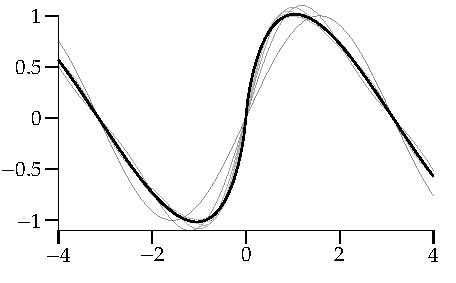
\includegraphics{figures/fouriersern2}
\caption{Plot of 
$\sum_{n=1}^\infty \frac{\sin(n x)}{n^2}$ including
the first 8 partial sums in various shades of gray.\label{fig:fouriersern2}}
\end{myfigureht}

\begin{example}
The series
\begin{equation*}
\sum_{n=0}^\infty \frac{x^n}{n!} 
\end{equation*}
converges uniformly on every bounded interval.
This series is a power series that we will study shortly.
Proof: Take the interval $[-r,r] \subset \R$ (every bounded interval
is contained in some $[-r,r]$).
The series $\sum_{n=0}^\infty \frac{r^n}{n!}$ converges by the ratio test,
so $\sum_{n=0}^\infty \frac{x^n}{n!}$ converges uniformly on $[-r,r]$ as
\begin{equation*}
\abs{\frac{x^n}{n!} } \leq 
\frac{r^n}{n!} .
\end{equation*}
\end{example}

Now we would love to say something about the limit.  For example, is it
continuous?


\begin{prop} \label{prop:uniformswitch}
Let $(X,d_X)$ and $(Y,d_Y)$ be metric spaces, and suppose $(Y,d_Y)$ is
Cauchy-complete.
Suppose $f_n \colon X \to Y$ converge uniformly to
 $f \colon X \to Y$.  
Let $\{ x_k \}_{k=1}^\infty$ be a sequence in $X$ and $x \coloneqq \lim_{k \to \infty} x_k$.  Suppose
\begin{equation*}
a_n \coloneqq \lim_{k \to \infty} f_n(x_k)
\end{equation*}
exists for all $n$.  Then
$\{a_n\}_{n=1}^\infty$ converges and 
\begin{equation*}
\lim_{k \to \infty} f(x_k) = \lim_{n\to\infty} a_n .
\end{equation*}
\end{prop}

In other words,
\begin{equation*}
\lim_{k \to \infty} \lim_{n\to\infty} f_n(x_k) =
\lim_{n \to \infty} \lim_{k\to\infty} f_n(x_k) .
\end{equation*}

\begin{proof}
First we show that $\{ a_n \}_{n=1}^\infty$ converges.  As
$\{ f_n \}_{n=1}^\infty$ converges uniformly it is uniformly Cauchy. 
Let $\epsilon > 0$ be given.  There is
an $M$ such that for all $m,n \geq M$, we have
\begin{equation*}
d_Y\bigl(f_n(x_k),f_m(x_k)\bigr) < \epsilon \qquad \text{for all } k .
\end{equation*}
Note that
$d_Y(a_n,a_m) \leq
d_Y\bigl(a_n,f_n(x_k)\bigr) +
d_Y\bigl(f_n(x_k),f_m(x_k)\bigr) +
d_Y\bigl(f_m(x_k),a_m\bigr)$ and take the limit as $k \to \infty$ to find
\begin{equation*}
d_Y(a_n,a_m) \leq \epsilon .
\end{equation*}
Hence $\{a_n\}_{n=1}^\infty$ is Cauchy and converges since $Y$ is complete.  Write
$a \coloneqq \lim_{k \to \infty} a_n$.

Find a $k \in \N$ such that
\begin{equation*}
d_Y\bigl(f_k(p),f(p)\bigr) < \nicefrac{\epsilon}{3}
\end{equation*}
for all $p \in X$.  Assume $k$ is large enough
so that
\begin{equation*}
d_Y(a_k,a) < \nicefrac{\epsilon}{3}  .
\end{equation*}
Find an $N \in \N$ such that for $m \geq N$,
\begin{equation*}
d_Y\bigl(f_k(x_m),a_k\bigr) < \nicefrac{\epsilon}{3}  .
\end{equation*}
Then for
$m \geq N$,
\begin{equation*}
d_Y\bigl(f(x_m),a\bigr)
\leq
d_Y\bigl(f(x_m),f_k(x_m)\bigr)
+
d_Y\bigl(f_k(x_m),a_k\bigr)
+
d_Y\bigl(a_k,a\bigr)
<
\nicefrac{\epsilon}{3} +
\nicefrac{\epsilon}{3} +
\nicefrac{\epsilon}{3} = \epsilon . \qedhere
\end{equation*}
\end{proof}

We obtain an immediate corollary about continuity.
If $f_n$ are all continuous then $a_n = f_n(x)$ and 
so $\{ a_n \}_{n=1}^\infty$ converges automatically to
$f(x)$ and so we do not require completeness of $Y$.

\begin{cor} \label{cor:metricuniformcontinuous}
Let $X$ and $Y$ be metric spaces.
If $f_n \colon X \to Y$ are continuous functions
such that
$\{ f_n \}_{n=1}^\infty$ converges uniformly to $f \colon X \to Y$,
then $f$ is continuous.
\end{cor}

The converse is not true.  Just because the limit is continuous does not mean
that the convergence is uniform.  For example:
$f_n \colon (0,1) \to \R$ defined by $f_n(x) \coloneqq x^n$ converge to
the zero function, but not uniformly.  However, if we add extra conditions
on the sequence, we can obtain a partial converse such as Dini's theorem,
\volIref{see \exerciseref*{vI-exercise:dinisthm} from volume I}{see \exerciseref{exercise:dinisthm}}.

In \exerciseref{exercise:CXCnormedspace} the reader is asked to prove
that for a compact $X$, $C(X,\C)$ is a normed vector space
with the uniform norm, and hence a metric space.  We have just shown that
$C(X,\C)$ is Cauchy-complete:  \propref{prop:unifcauchymetric} says that a Cauchy
sequence in $C(X,\C)$ converges uniformly to some function,
and \corref{cor:metricuniformcontinuous} shows that the limit is
continuous and hence in $C(X,\C)$.

\begin{cor}
Let $(X,d)$ be a compact metric space.
Then $C(X,\C)$ is a Cauchy-complete metric space.
\end{cor}

\begin{example}
By \exampleref{example:sinnsqfourier}
the Fourier series 
\begin{equation*}
\sum_{n=1}^\infty \frac{\sin(nx)}{n^2}
\end{equation*}
converges uniformly and hence is continuous by \corref{cor:metricuniformcontinuous} (as is visible
in \figureref{fig:fouriersern2}).
\end{example}

\subsection{Integration}

\begin{prop} \label{prop:complexlimitswapintegral}
Suppose $f_n \colon [a,b] \to \C$
are Riemann integrable and suppose that $\{ f_n \}_{n=1}^\infty$ converges
uniformly to $f \colon [a,b] \to \C$.  Then $f$ is Riemann integrable
and
\begin{equation*}
\int_a^b f = \lim_{n\to \infty} \int_a^b f_n .
\end{equation*}
\end{prop}

Since the integral of a complex-valued function is just the integral of
the real and imaginary parts separately,
the proof follows directly by the results of
\volIref{\chapterref*{vI-fs:chapter} of volume~I}{\chapterref{fs:chapter}}.
We leave the details as an exercise.

\begin{cor}
\pagebreak[2]
Suppose $f_n \colon [a,b] \to \C$
are Riemann integrable and suppose that
\begin{equation*}
\sum_{n=1}^\infty f_n(x)
\end{equation*}
converges uniformly.  Then the series is Riemann integrable on $[a,b]$
and
\begin{equation*}
\int_a^b \sum_{n=1}^\infty f_n(x) \,dx
=
\sum_{n=1}^\infty \int_a^b f_n(x) \,dx
\end{equation*}
\end{cor}

\begin{example}
Let us show how to integrate a Fourier series.
\begin{equation*}
\int_{0}^x \sum_{n=1}^\infty \frac{\cos(nt)}{n^2} \,dt
=
\sum_{n=1}^\infty \int_{0}^x \frac{\cos(nt)}{n^2}\,dt
=
\sum_{n=1}^\infty \frac{\sin(nx)}{n^3}
\end{equation*}
The swapping of integral and sum is possible because of uniform convergence,
which we have proved before using the Weierstrass $M$-test
(\thmref{thm:weiermtest}).
\end{example}

We remark that we can swap integrals and limits under far less stringent hypotheses,
but for that we would need a stronger integral than the Riemann integral.
E.g.\ the Lebesgue integral.

\subsection{Differentiation}

Recall that a complex-valued function
$f \colon [a,b] \to \C$, where $f(x) = u(x)+i\,v(x)$,
is differentiable, if $u$ and $v$ are differentiable
and the derivative is
\begin{equation*}
f'(x) = u'(x)+i\,v'(x) .
\end{equation*}

The proof of the following theorem is to apply the corresponding theorem for
real functions to $u$ and $v$, and is left as an exercise.

\begin{thm} \label{thm:dersconvergecomplex}
Let $I \subset \R$ be a bounded interval and let
$f_n \colon I \to \C$ be continuously differentiable functions.
Suppose $\{ f_n' \}_{n=1}^\infty$ converges uniformly to $g \colon I \to \C$,
and suppose $\{ f_n(c) \}_{n=1}^\infty$ is a
convergent sequence for some $c \in I$.  Then $\{ f_n \}_{n=1}^\infty$ converges uniformly to 
a continuously differentiable function $f \colon I \to \C$, and $f' = g$.
\end{thm}

Uniform limits of the functions themselves are not enough, and can make
matters even worse.  In \sectionref{sec:stoneweier} we will prove that
continuous functions are uniform limits of polynomials, yet as the following
example demonstrates, a continuous function need not be differentiable
anywhere.

\begin{example}
There exist continuous nowhere differentiable functions.
Such functions are often called
\emph{Weierstrass functions}\index{Weierstrass function},
although this
particular one, essentially due to
Takagi\footnote{\href{https://en.wikipedia.org/wiki/Teiji_Takagi}{Teiji
Takagi} (1875--1960) was a Japanese mathematician.}, is a different example than what Weierstrass gave.
Define
\begin{equation*}
\varphi(x) \coloneqq \sabs{x} \qquad \text{for } x \in [-1,1] .
\end{equation*}
Extend $\varphi$ to all of $\R$ by making it
2-periodic:
Decree that
$\varphi(x) = \varphi(x+2)$.  The function $\varphi \colon \R \to \R$
is continuous, in fact, $\sabs{\varphi(x)-\varphi(y)} \leq \sabs{x-y}$ (why?).
See \figureref{fig:triangwave}.
\begin{myfigureht}
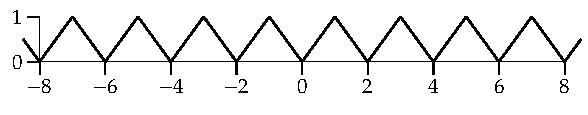
\includegraphics{figures/triangwave}
\caption{The 2-periodic function $\varphi$.\label{fig:triangwave}}
\end{myfigureht}

As $\sum_{n=0}^\infty {\left(\frac{3}{4}\right)}^n$ converges and $\sabs{\varphi(x)} \leq
1$ for all $x$, by the $M$-test
(\thmref{thm:weiermtest}),
\begin{equation*}
f(x) \coloneqq \sum_{n=0}^\infty 
{\left(\frac{3}{4}\right)}^n \varphi(4^n x)
\end{equation*}
converges uniformly and hence is continuous.
See \figureref{fig:nowherediff}.

\begin{myfigureht}
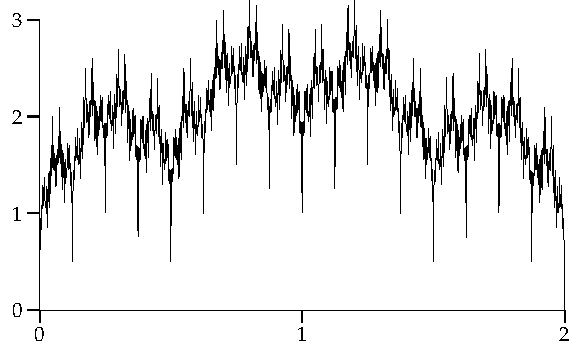
\includegraphics{figures/nowherediff}
\caption{Plot of the nowhere differentiable function $f$.\label{fig:nowherediff}}
\end{myfigureht}

We claim $f \colon
\R \to \R$ is nowhere differentiable.
Fix $x$, and we will show $f$ is not differentiable at $x$.
Define
\begin{equation*}
\delta_m \coloneqq \pm \frac{1}{2} 4^{-m} ,
\avoidbreak
\end{equation*}
where the sign is chosen so that there is no integer
between $4^m x$ and $4^m(x+\delta_m) = 4^m x \pm \frac{1}{2}$.

We want to look at the difference quotient
\begin{equation*}
\frac{f(x+\delta_m)-f(x)}{\delta_m}
=
\sum_{n=0}^\infty 
{\left(\frac{3}{4}\right)}^n
\frac{\varphi\bigl(4^n(x+\delta_m)\bigr)-\varphi(4^nx)}{\delta_m} .
\end{equation*}
Fix $m$ for a moment.  Consider the expression inside the series:
\begin{equation*}
\gamma_{n} \coloneqq
\frac{\varphi\bigl(4^n(x+\delta_m)\bigr)-\varphi(4^nx)}{\delta_m} .
\end{equation*}
If $n > m$, then $4^n\delta_m$ is an even integer.  As $\varphi$
is 2-periodic we get that $\gamma_n = 0$.

As there is no integer between 
$4^m(x+\delta_m) = 4^m x\pm\nicefrac{1}{2}$ and $4^m x$, then on this interval
$\varphi(t) = \pm t + \ell$ for some integer $\ell$.
In particular,
$\abs{\varphi\bigl(4^m(x+ \delta_m)\bigr)-\varphi(4^mx)} =
\abs{4^mx\pm\nicefrac{1}{2}-4^mx} = \nicefrac{1}{2}$.  Therefore,
\begin{equation*}
\sabs{\gamma_m} =
\abs{
\frac{\varphi\bigl(4^m(x+\delta_m)\bigr)-\varphi(4^mx)}{\pm (\nicefrac{1}{2}) 4^{-m}}
}
= 4^m .
\end{equation*}
Similarly, suppose $n < m$.  Since $\sabs{\varphi(s) -\varphi(t)} \leq
\sabs{s-t}$,
\begin{equation*}
\sabs{\gamma_n} =
\abs{\frac{\varphi\bigl(4^nx\pm(\nicefrac{1}{2})4^{n-m}\bigr)-\varphi(4^nx)}{\pm
(\nicefrac{1}{2}) 4^{-m}}}
\leq
\abs{\frac{\pm(\nicefrac{1}{2})4^{n-m}}{\pm (\nicefrac{1}{2}) 4^{-m}}} = 4^n
.
\end{equation*}

And so
\begin{equation*}
\begin{split}
\abs{
\frac{f(x+\delta_m)-f(x)}{\delta_m}
}
%& =
%\abs{
%\sum_{n=0}^\infty 
%{\left(\frac{3}{4}\right)}^n
%\frac{\varphi\bigl(4^n(x+\delta_m)\bigr)-\varphi(4^nx)}{\delta_m}
%}
=
\abs{
\sum_{n=0}^\infty 
{\left(\frac{3}{4}\right)}^n
\gamma_n
}
& =
\abs{
\sum_{n=0}^m 
{\left(\frac{3}{4}\right)}^n
\gamma_n
}
\\
& \geq
\abs{
{\left(\frac{3}{4}\right)}^m
\gamma_m}
-
\abs{
\sum_{n=0}^{m-1} 
{\left(\frac{3}{4}\right)}^n
\gamma_n
}
\\
& \geq
3^m
-
\sum_{n=0}^{m-1} 
3^n
=
3^m
-
\frac{3^{m}-1}{3-1}
=
\frac{3^m +1}{2} .
\end{split}
\end{equation*}
As $m \to \infty$, we have
$\delta_m \to 0$, but $\frac{3^m+1}{2}$
goes to infinity.  So $f$ cannot be differentiable at~$x$.
\end{example}

\subsection{Exercises}

\begin{exercise}
Prove \propref{prop:uniformconvbounded}.
\end{exercise}

\begin{exercise}
Prove \propref{prop:unifcauchymetric}.
\end{exercise}

\begin{exercise} \label{exercise:CXCnormedspace}
Suppose $(X,d)$ is a compact metric space.
Prove that the uniform norm $\snorm{\cdot}_X$ is a norm on the vector space of
continuous complex-valued functions $C(X,\C)$.
\end{exercise}

\begin{exercise}
\pagebreak[2]
\leavevmode
\begin{enumerate}[a)]
\item
Prove that
$f_n(x) \coloneqq 2^{-n} \sin(2^n x)$
converge uniformly to zero, but there exists a dense set $D \subset \R$
such that $\lim_{n\to\infty} f_n'(x) = 1$ for all $x \in D$.
\item
Prove that
$\sum_{n=1}^\infty 2^{-n} \sin(2^n x)$
converges uniformly to a continuous function,
and there exists a dense set $D \subset \R$
where the derivatives of the partial sums do not converge.
\end{enumerate}
\end{exercise}

\begin{exercise}
Prove that $\snorm{f}_{C^1} \coloneqq \snorm{f}_{[a,b]}+\snorm{f'}_{[a,b]}$
is a norm on the vector space of
continuously differentiable complex-valued functions $C^1\bigl([a,b],\C\bigr)$.
\end{exercise}

\begin{exercise}
Prove \thmref{thm:dersconvergecomplex}.
\end{exercise}

\begin{exercise}
Prove \propref{prop:complexlimitswapintegral} by reducing to the real
result.
\end{exercise}

\begin{exercise}
Work through the following counterexample to the converse of
the Weierstrass $M$-test (\thmref{thm:weiermtest}).  Define
$f_n \colon [0,1] \to \R$ by
\begin{equation*}
f_n(x) \coloneqq
\begin{cases}
\frac{1}{n} & \text{if } \frac{1}{n+1} < x < \frac{1}{n},\\
0	    & \text{else.}
\end{cases}
\end{equation*}
Prove that $\sum_{n=1}^\infty f_n$ converges uniformly, but
$\sum_{n=1}^\infty \snorm{f_n}_{[0,1]}$
does not converge.
\end{exercise}

\begin{exercise}
Suppose $f_n \colon [0,1] \to \R$ are monotone increasing functions and
suppose that $\sum_{n=1}^\infty f_n$ converges pointwise.  Prove that
$\sum_{n=1}^\infty f_n$
converges uniformly.
\end{exercise}

\begin{exercise}
Prove that
\begin{equation*}
\sum_{n=1}^\infty e^{-nx}
\end{equation*}
converges for all $x > 0$ to a differentiable function.
\end{exercise}

%%%%%%%%%%%%%%%%%%%%%%%%%%%%%%%%%%%%%%%%%%%%%%%%%%%%%%%%%%%%%%%%%%%%%%%%%%%%%%

\sectionnewpage
\section{Power series and analytic functions}
\label{sec:analfuncs}

\sectionnotes{2--3 lectures}

\subsection{Analytic functions}

A (complex) power series is a series of the form
\begin{equation*}
\sum_{n=0}^\infty c_n {(z-a)}^n
\end{equation*}
for $c_n, z, a \in \C$.  We say the series
\emph{converges}\index{converges!power series} if the series converges for
some $z \not= a$.

Let $U \subset \C$ be an open set and
$f \colon U \to \C$ a function.
Suppose that for every $a \in U$ there exists a $\rho > 0$ and a power
series convergent to the function
\begin{equation*}
f(z) = \sum_{n=0}^\infty c_n {(z-a)}^n
\end{equation*}
for all $z \in B(a,\rho)$.
Then we say $f$ is an \emph{\myindex{analytic}} function.

Similarly, given an interval $(a,b) \subset \R$, we say that $f \colon (a,b) \to \C$
is analytic or perhaps \emph{\myindex{real-analytic}}
if for each point $c \in
(a,b)$ there is a power series around $c$ that converges in some
$(c-\rho,c+\rho)$
for some $\rho > 0$.

As we will sometimes talk about real and sometimes about complex power
series, we will use $z$ to denote a complex number and $x$ a real number.
We will always mention which case we are working with.

An analytic function has different expansions around different points.
Moreover, convergence does not automatically happen on the entire
domain of the function.  For example, if $\sabs{z} < 1$, then
\begin{equation*}
\frac{1}{1-z} = \sum_{n=0}^\infty z^n .
\end{equation*}
While the left-hand side exists on all of $z \not= 1$, the right-hand side
happens to converge only if $\sabs{z} < 1$.  See a graph
of a small piece of $\frac{1}{1-z}$ in \figureref{fig:1over1mz}.
We cannot graph the
function itself, we can only graph its real or imaginary parts for lack
of dimensions in our universe.

\begin{myfigureht}
\subimport*{figures/}{real_imag_1over1mz.pdf_t}
\caption{Graphs of the real and imaginary parts of $z=x+iy \mapsto \frac{1}{1-z}$
in the square $[-0.8,0.8]^2$.  The singularity at $z=1$ is marked with a
vertical dashed line.\label{fig:1over1mz}}
\end{myfigureht}

\subsection{Convergence of power series}

We proved several results for power series of a real variable in
\volIref{\sectionref*{vI-sec:moreonseries} of volume I}{\sectionref{sec:moreonseries}}.   For the most part the convergence
properties of power series deal with the series
$\sum_{k=0}^\infty \sabs{c_k} \, \sabs{z-a}^k$
and so we have already proved many results about complex power
series.  In particular, we computed the so-called
radius of convergence of a power series.

\begin{samepage}
\begin{prop}
Let $\sum_{n=0}^\infty c_n {(z-a)}^n$ be a power series.
There exists a $\rho \in [0,\infty]$ such that
\begin{enumerate}[(i)]
\item If $\rho = 0$, then the series diverges.
\item If $\rho = \infty$, then the series converges absolutely for all $z \in \C$.
\item If $0 < \rho < \infty$, then the
series converges absolutely on $B(a,\rho)$,
and diverges when $\sabs{z-a} > \rho$.
\end{enumerate}
Furthermore, if $0 < r < \rho$, then
the series converges uniformly on the closed ball $C(a,r)$.
\end{prop}
\end{samepage}

The number $\rho$ is the \emph{\myindex{radius of convergence}}.
See \figureref{fig:radiusconvcomplex}.
The radius of convergence gives a disc around $a$ where the series converges.  A power series
is convergent if $\rho > 0$.
\begin{myfigureht}
\subimport*{figures/}{radiusconvcomplex.pdf_t}
\caption{Radius of convergence.\label{fig:radiusconvcomplex}}
\end{myfigureht}

\begin{proof}
We use the real version of this proposition,
\volIref{\propref*{vI-prop:powerserrealradius} in volume I}{\propref{prop:powerserrealradius}}.
Let
\begin{equation*}
R \coloneqq \limsup_{n\to\infty} \sqrt[n]{\sabs{c_n}} .
\end{equation*}
If $R = 0$, then
$\sum_{n=0}^\infty \sabs{c_n} \, \sabs{z-a}^n$ converges for all $z$.
If $R = \infty$, then
$\sum_{n=0}^\infty \sabs{c_n} \, \sabs{z-a}^n$ converges only at $z=a$.
Otherwise, let $\rho \coloneqq \nicefrac{1}{R}$ and
$\sum_{n=0}^\infty \sabs{c_n} \, \sabs{z-a}^n$ converges when
$\sabs{z-a} < \rho$, and diverges (in fact the terms of the series
do not go to zero) when $\sabs{z-a} > \rho$.

To prove the ``Furthermore,'' suppose
$0 < r < \rho$ and $z \in C(a,r)$.  Then
consider the partial sums
\begin{equation*}
\abs{\sum_{n=0}^k c_n {(z-a)}^n}
\leq
\sum_{n=0}^k \sabs{c_n} \sabs{z-a}^n
\leq
\sum_{n=0}^k \sabs{c_n} r^n . \qedhere
\end{equation*}
\end{proof}

If $\sum_{n=0}^\infty c_n {(z-a)}^n$ converges for some $z$, then
\begin{equation*}
\sum_{n=0}^\infty c_n {(w-a)}^n
\end{equation*}
converges absolutely whenever $\sabs{w-a} < \sabs{z-a}$.
Conversely if the series diverges at $z$, then it must diverge at $w$
whenever $\sabs{w-a} > \sabs{z-a}$.
Hence, to show
that the radius of convergence is at least some number, we simply need to
show convergence at some point by any method we know.

\begin{example}
We list some series we already know:
\begin{align*}
& &
& \sum_{n=0}^\infty z^n
& & \text{has radius of convergence } 1.
& &
\\
& &
& \sum_{n=0}^\infty \frac{1}{n!} z^n
& & \text{has radius of convergence } \infty.
& &
\\
& &
& \sum_{n=0}^\infty n^n z^n
& & \text{has radius of convergence } 0.
& &
\end{align*}
\end{example}

\begin{example}
Note the difference between $\frac{1}{1-z}$ and its power series.  Let us
expand $\frac{1}{1-z}$ as power series around a point $a \not= 1$.
Let $c \coloneqq \frac{1}{1-a}$, then
\begin{equation*}
\frac{1}{1-z} = 
\frac{c}{1-c(z-a)}
=
c
\sum_{n=0}^\infty c^{n} {(z-a)}^n
=
\sum_{n=0}^\infty \left( \frac{1}{{(1-a)}^{n+1}} \right) {(z-a)}^n .
\end{equation*}
The series $\sum_{n=0}^\infty c^n {(z-a)}^n$ converges if and only if 
the series on the right-hand side converges and
\begin{equation*}
\limsup_{n\to\infty}
\sqrt[n]{\sabs{c^n}} = \sabs{c}
= \frac{1}{\sabs{1-a}} .
\end{equation*}
The radius of convergence of the power series is $\sabs{1-a}$, that is the
distance from $1$ to $a$.  The function $\frac{1}{1-z}$
has a power series
representation around every $a\not= 1$ and so is analytic in $\C \setminus
\{ 1 \}$.
The domain of the function is bigger than the region
of convergence of the power series representing the function at any point.
\end{example}

It turns out that 
if a function has a power series representation converging to the function
on some ball,
then it has a power series representation at every point in the ball.  We will prove this
result later.

\subsection{Properties of analytic functions}

\begin{prop}
If
\begin{equation*}
f(z) \coloneqq \sum_{n=0}^\infty c_n {(z-a)}^n
\end{equation*}
is convergent in $B(a,\rho)$ for some $\rho > 0$, then
$f \colon B(a,\rho) \to \C$ is continuous.
In particular, analytic functions are continuous.
\end{prop}

\begin{proof}
For $z_0 \in B(a,\rho)$, pick $r < \rho$ such that $z_0 \in B(a,r)$.
On $B(a,r)$ the
partial sums (which are continuous) converge uniformly,
and so the limit $f|_{B(a,r)}$ is continuous.
Any sequence converging to
$z_0$ has some tail that is completely in the open ball $B(a,r)$,
hence $f$ is continuous at $z_0$.
\end{proof}

In \volIref{\corref*{vI-cor:differentiatepowerser} of volume
I}{\corref{cor:differentiatepowerser}}, we proved that we can
differentiate real power series term by term.  That is,
we proved that if
\begin{equation*}
f(x) \coloneqq \sum_{n=0}^\infty c_n {(x-a)}^n
\end{equation*}
converges for real $x$ in an interval around $a \in \R$, then we can differentiate
term by term and obtain a series
\begin{equation*}
f'(x) =
\sum_{n=1}^\infty n c_n {(x-a)}^{n-1}
=
\sum_{n=0}^\infty (n+1)c_{n+1} {(x-a)}^{n} 
\end{equation*}
with the same radius of convergence.
We only proved this theorem when $c_n$ is real, however, for complex $c_n$,
we write
$c_n = s_n + i t_n$, and as $x$ and $a$ are real
\begin{equation*}
\sum_{n=0}^\infty c_n {(x-a)}^n
=
\sum_{n=0}^\infty s_n {(x-a)}^n
+
i
\sum_{n=0}^\infty t_n {(x-a)}^n .
\end{equation*}
We apply the theorem to the real and
imaginary part.

By iterating this theorem, we find that an
analytic function is infinitely differentiable:
\begin{equation*}
f^{(\ell)}(x) =
\sum_{n=\ell}^\infty n(n-1)\cdots(n-\ell+1)c_k {(x-a)}^{n-\ell}
=
\sum_{n=0}^\infty (n+\ell)(n+\ell-1)\cdots (n+1) c_{n+\ell} {(x-a)}^{n} .
\end{equation*}
In particular,
\begin{equation} \label{eq:formulaforpscoeffs}
f^{(\ell)}(a) = \ell! \, c_\ell .
\avoidbreak
\end{equation}
The coefficients are uniquely determined by the derivatives of the
function, and vice versa.

On the other hand, just because we have an infinitely differentiable
function doesn't mean that the numbers $c_n$ obtained by
$c_n = \frac{f^{(n)}(0)}{n!}$ give a convergent power series.
There is a theorem, which we will not prove,
that given an arbitrary sequence $\{ c_n \}_{n=1}^\infty$, there exists an
infinitely differentiable function $f$ such that
$c_n = \frac{f^{(n)}(0)}{n!}$.  Moreover, even if the obtained series
converges, it may not converge to the function we started with.
For an example,
see \volIref{\exerciseref*{vI-exercise:nonanalytic} in volume I}{\exerciseref{exercise:nonanalytic}}:  The
function
\begin{equation*}
f(x) \coloneqq
\begin{cases}
e^{-1/x} & \text{if } x > 0,\\
0        & \text{if } x \leq 0,
\end{cases}
\end{equation*}
is infinitely differentiable, and all derivatives at the origin are zero.
So
its series at the origin would be just the zero series, and while that
series converges, it does not converge to~$f$ for $x > 0$.

\medskip

We can apply an affine transformation $z \mapsto z+a$ that
converts a power series at $a$ to a series at the origin.
That is, if
\begin{equation*}
f(z) = \sum_{n=0}^\infty c_n {(z-a)}^n,
\qquad \text{we consider} \qquad
f(z+a) = \sum_{n=0}^\infty c_n {z}^n.
\end{equation*}
Therefore, it is usually
sufficient to prove results about power series at the origin.
From now on, we often assume $a=0$ for simplicity.

\subsection{Power series as analytic functions}

We need a theorem on swapping limits of series, that is, 
Fubini's theorem for sums.  For real series this was
\volIref{\exerciseref*{vI-exercise:tonellifubiniforsums} in volume
I}{\exerciseref{exercise:tonellifubiniforsums}}, but we have a slicker
argument now.

\begin{thm}[\myindex{Fubini for sums}] \label{thm:fubiniforsums}
Let $\{ a_{k,m} \}_{k=1,m=1}^\infty$ be a double
sequence of complex numbers and suppose that for every $k$ the series
\begin{equation*}
\sum_{m=1}^\infty \sabs{a_{k,m}} \qquad \text{converges}
\end{equation*}
and furthermore that
\begin{equation*}
\sum_{k=1}^\infty \left( \sum_{m=1}^\infty \sabs{a_{k,m}} \right)
\qquad \text{converges}.
\end{equation*}
Then
\begin{equation*}
\sum_{k=1}^\infty \left( \sum_{m=1}^\infty a_{k,m} \right)
=
\sum_{m=1}^\infty \left( \sum_{k=1}^\infty a_{k,m} \right) ,
\end{equation*}
where all the series involved converge.
\end{thm}

\begin{proof}
Let $E$ be the set $\{ \nicefrac{1}{n} : n \in \N \} \cup \{ 0 \}$,
and treat it as a metric space with the metric inherited from $\R$.
Define the sequence of functions $f_k \colon E \to \C$
by
\begin{equation*}
f_k(\nicefrac{1}{n}) \coloneqq \sum_{m=1}^n a_{k,m}
\qquad
\text{and}
\qquad
f_k(0) \coloneqq \sum_{m=1}^\infty a_{k,m} .
\end{equation*}
As the series converges, each $f_k$ is continuous at $0$
(since 0 is the only cluster point, they are continuous at every point of
$E$, but we don't need that).
For all $x \in E$, we have
\begin{equation*}
\sabs{f_k(x)} \leq \sum_{m=1}^\infty \sabs{a_{k,m}} .
\end{equation*}
As $\sum_k \sum_m \sabs{a_{k,m}}$ converges (and does not depend on
$x$), we know that
\begin{equation*}
\sum_{k=1}^n f_k(x)
\end{equation*}
converges uniformly on $E$.  Define
\begin{equation*}
g(x) \coloneqq \sum_{k=1}^\infty f_k(x) ,
\end{equation*}
which is, therefore, a continuous function at $0$.
So
\begin{equation*}
\begin{split}
\sum_{k=1}^\infty \left( \sum_{m=1}^\infty a_{k,m} \right)
& =
\sum_{k=1}^\infty f_k(0)
= g(0)
= \lim_{n\to\infty} g(\nicefrac{1}{n}) \\
&= 
\lim_{n\to\infty}\sum_{k=1}^\infty f_k(\nicefrac{1}{n})
= 
\lim_{n\to\infty}\sum_{k=1}^\infty \sum_{m=1}^n a_{k,m} \\
&= 
\lim_{n\to\infty}\sum_{m=1}^n \sum_{k=1}^\infty a_{k,m}
= 
\sum_{m=1}^\infty \left( \sum_{k=1}^\infty a_{k,m} \right) . \qedhere
\end{split}
\end{equation*}
\end{proof}

Now we prove that once we have a series converging to a function
in some interval, we can expand the function around every point.

\begin{thm}[Taylor's theorem for real-analytic functions]
\index{Taylor's theorem!real-analytic}%
\label{thm:tayloranal}
Let
\begin{equation*}
f(x) \coloneqq \sum_{k=0}^\infty a_k x^k
\end{equation*}
be a power series converging in $(-\rho,\rho)$ for some $\rho > 0$.  Given any $a \in
(-\rho,\rho)$,
and $x$ such that $\sabs{x-a} < \rho-\sabs{a}$, we obtain
\begin{equation*}
f(x) =
\sum_{k=0}^\infty \frac{f^{(k)}(a)}{k!} {(x-a)}^{k} .
\end{equation*}
\end{thm}

The power series at $a$ could of course converge in a larger interval, but
the one above is guaranteed.  It is the largest symmetric interval about
$a$ that fits in $(-\rho,\rho)$.

\begin{proof}
Given $a$ and $x$ as in the theorem,
write
\begin{equation*}
\begin{split}
f(x) &= \sum_{k=0}^\infty a_k {\bigl((x-a)+a\bigr)}^k \\
&= \sum_{k=0}^\infty a_k \sum_{m=0}^k \binom{k}{m} a^{k-m} {(x-a)}^m .
\end{split}
\end{equation*}
Define $c_{k,m} \coloneqq a_k \binom{k}{m} a^{k-m}$ if $m \leq k$ and $0$ if $m >
k$.  Then 
\begin{equation} \label{eq:tsproof}
f(x) = \sum_{k=0}^\infty \, \sum_{m=0}^\infty c_{k,m} {(x-a)}^m .
\end{equation}
Let us show that the double sum converges absolutely.
\begin{equation*}
\begin{split}
\sum_{k=0}^\infty \, \sum_{m=0}^\infty \abs{ c_{k,m} {(x-a)}^m}
& = \sum_{k=0}^\infty \, \sum_{m=0}^k \abs{ a_k \binom{k}{m} a^{k-m} {(x-a)}^m }
\\
& = \sum_{k=0}^\infty \sabs{a_k} \sum_{m=0}^k \binom{k}{m} \sabs{a}^{k-m}
{\sabs{x-a}}^m  \\
& = \sum_{k=0}^\infty \sabs{a_k} {\bigl(\sabs{x-a}+\sabs{a}\bigr)}^k ,
\end{split}
\end{equation*}
and this series converges as long as 
$(\sabs{x-a}+\sabs{a}) < \rho$ or in other words if
$\sabs{x-a} < \rho-\sabs{a}$.

Using \thmref{thm:fubiniforsums},
swap the order of summation in \eqref{eq:tsproof}, and 
the following series converges when $\sabs{x-a} < \rho-\sabs{a}$:
\begin{equation*}
f(x) =
\sum_{k=0}^\infty \, \sum_{m=0}^\infty c_{k,m} {(x-a)}^m
=
\sum_{m=0}^\infty
\left( \sum_{k=0}^\infty
c_{k,m} \right) {(x-a)}^m .
\end{equation*}
The formula in terms of derivatives at $a$ follows by
differentiating the series to obtain \eqref{eq:formulaforpscoeffs}.
\end{proof}

Note that if a series converges for real $x \in (a-\rho,a+\rho)$ it also converges
for all complex numbers in $B(a,\rho)$.
We have the following corollary, which says that functions defined
by power series are analytic.

\begin{cor} \label{cor:powerseranalytic}
For every $a \in \C$,
if $\sum_{k=0}^\infty c_k {(z-a)}^k$ converges to $f(z)$ in $B(a,\rho)$ and $b \in
B(a,\rho)$,
then there exists a power series
$\sum_{k=0}^\infty d_k {(z-b)}^k$ that converges to $f(z)$ in $B(b,\rho-\sabs{b-a})$.
\end{cor}

\begin{proof}
Without loss of generality assume that $a=0$.  We can rotate to assume that $b$ is real, but
since that is harder to picture, let us do it explicitly.
Let $\alpha \coloneqq \frac{\bar{b}}{\sabs{b}}$.
Notice that
\begin{equation*}
\abs{\nicefrac{1}{\alpha}} = \sabs{\alpha}
= 1 .
\end{equation*}
Therefore the series
$\sum_{k=0}^\infty c_k {(\nicefrac{z}{\alpha})}^k = 
\sum_{k=0}^\infty c_k \alpha^{-k} {z}^k$
converges to $f(\nicefrac{z}{\alpha})$ in $B(0,\rho)$.
When $z=x$ is real
we apply \thmref{thm:tayloranal} at $\sabs{b}$ and get
a series that converges
to $f(\nicefrac{z}{\alpha})$ on $B(\sabs{b},\rho-\sabs{b})$.
That is, there is a convergent series
\begin{equation*}
f(\nicefrac{z}{\alpha}) =
\sum_{k=0}^\infty a_k {\bigl(z - \sabs{b}\bigr)}^k .
\end{equation*}
Using $\alpha b = \sabs{b}$, we find
\begin{equation*}
f(z) = f(\nicefrac{\alpha z}{\alpha}) =
\sum_{k=0}^\infty a_k {(\alpha z - \sabs{b})}^k 
=
\sum_{k=0}^\infty a_k\alpha^k {\bigl(z - \nicefrac{\sabs{b}}{\alpha}\bigr)}^k
=
\sum_{k=0}^\infty a_k\alpha^k {(z - b)}^k ,
\end{equation*}
and this series converges for all $z$ such that
$\bigl\lvert \alpha z-\sabs{b}\bigr\rvert < \rho-\sabs{b}$
or $\sabs{z - b} < \rho-\sabs{b}$.
\end{proof}

We proved above that a convergent power series is an
analytic function where it converges.  We have also shown before that
$\frac{1}{1-z}$ is analytic outside of $z=1$.

Note that just because a real analytic function is analytic on the
entire real line it does not necessarily mean that it has a power series
representation that converges everywhere.  For example, the function
\begin{equation*}
f(x) = \frac{1}{1+x^2}
\end{equation*}
happens to be real analytic function on $\R$ (exercise).  A power
series around the origin converging to $f$
has a radius of convergence of exactly $1$.
Can you see why? (exercise)

\subsection{Identity theorem for analytic functions}

\begin{lemma}
Suppose $f(z) = \sum_{k=0}^\infty a_k z^k$ is a convergent power series and
$\{ z_n \}_{n=1}^\infty$ is a sequence of nonzero complex numbers converging to 0,
such that $f(z_n) = 0$ for all $n$.  Then $a_k = 0$ for every~$k$.
\end{lemma}

\begin{proof}
By continuity we know $f(0) = 0$ so $a_0 = 0$.
Suppose there exists some nonzero $a_k$.
Let $m$ be the smallest $m$ such that $a_m \not= 0$.  Then
\begin{equation*}
f(z) = \sum_{k=m}^\infty a_k z^k = 
z^m \sum_{k=m}^\infty a_k z^{k-m} =
z^m \sum_{k=0}^\infty a_{k+m} z^{k} .
\end{equation*}
Write $g(z) = \sum_{k=0}^\infty a_{k+m} z^{k}$ (this series converges in
on the same set as $f$).  $g$ is continuous and $g(0) = a_m \not= 0$.  Thus
there exists some $\delta > 0$ such that $g(z) \not= 0$ for all $z \in
B(0,\delta)$.  As $f(z) = z^m g(z)$, the only point in $B(0,\delta)$ where
$f(z) = 0$ is when $z=0$, but this contradicts the assumption
that $f(z_n) = 0$ for all $n$.
\end{proof}

Recall that in a metric space $X$, a \emph{cluster point}
(or sometimes \emph{limit point}) of a set
$E$ is a point $p \in X$ such that
$B(p,\epsilon) \setminus \{ p \}$ contains points of $E$
for all $\epsilon > 0$.

\begin{thm}[Identity theorem]
\label{thm:identityanalytic}%
\index{identity theorem}%
Let $U \subset \C$ be open and connected.  If $f \colon U \to \C$
and $g \colon U \to \C$ are analytic functions that are
equal on a set $E \subset U$, and $E$ has a cluster point
in $U$, then $f(z) = g(z)$ for all $z \in U$.
\end{thm}

In most common applications of this theorem $E$ is an open set or perhaps a curve.

\begin{proof}
Without loss of generality suppose $E$ is the set of all points $z \in U$ such that
$g(z)=f(z)$.  Note that $E$ must be closed as $f$ and $g$ are continuous.

Suppose $E$ has a cluster point.  Without loss of generality assume that $0$
is this cluster point.  Near $0$,
we have the expansions
\begin{equation*}
f(z) = \sum_{k=0}^\infty a_k {z}^k 
\qquad
\text{and}
\qquad
g(z) = \sum_{k=0}^\infty b_k {z}^k ,
\end{equation*}
which converge in some ball $B(0,\rho)$.  Therefore the series
\begin{equation*}
0 = f(z)-g(z) = 
\sum_{k=0}^\infty (a_k-b_k) z^k
\end{equation*}
converges in $B(0,\rho)$.  As $0$ is a cluster point of $E$, there
is a sequence of nonzero points $\{ z_n \}_{n=1}^\infty$ such that
$f(z_n) -g(z_n) = 0$.  Hence, by the lemma above 
$a_k = b_k$ for all $k$.  Therefore, $B(0,\rho) \subset E$.

Thus the set of cluster points of $E$ is open.  The set of cluster points
of $E$ is also closed: A limit of cluster points of $E$ is in $E$
as it is closed, and it is clearly a cluster point of $E$.
As $U$ is connected, the set of cluster points of $E$
is equal to $U$, or in other words $E = U$.
\end{proof}

By restricting our attention to real $x$, we obtain the same
theorem for connected open subsets of $\R$, which are just open intervals.

\subsection{Exercises}

\begin{exercise}
Let
\begin{equation*}
a_{k,m} \coloneqq
\begin{cases}
1        & \text{if } k=m,\\
-2^{k-m} & \text{if } k<m,\\
0        & \text{if } k>m.
\end{cases}
\end{equation*}
Compute (or show the limit doesn't exist):
\\
a)~$\displaystyle \sum_{m=1}^\infty \sabs{a_{k,m}}~$ for all $k$,
%mbxSTARTIGNORE
\hspace{\fill}
%mbxENDIGNORE
%mbxlatex \qquad
b)~$\displaystyle \sum_{k=1}^\infty \sabs{a_{k,m}}~$ for all $m$,
%mbxSTARTIGNORE
\hspace{\fill}
%mbxENDIGNORE
%mbxlatex \qquad
c)~$\displaystyle \sum_{k=1}^\infty \sum_{m=1}^\infty \sabs{a_{k,m}}$,
%mbxSTARTIGNORE
\hspace{\fill}
%mbxENDIGNORE
%mbxlatex \qquad
d)~$\displaystyle \sum_{k=1}^\infty \sum_{m=1}^\infty a_{k,m}$,
%mbxSTARTIGNORE
\hspace{\fill}
%mbxENDIGNORE
%mbxlatex \qquad
e)~$\displaystyle \sum_{m=1}^\infty \sum_{k=1}^\infty a_{k,m}$.
\\
Hint: Fubini for sums does not apply, in fact, answers to
d) and e) are different.
\end{exercise}

\begin{exercise}
\pagebreak[2]
Let $f(x) \coloneqq \frac{1}{1+x^2}$.  Prove that
\begin{enumerate}[a)]
\item
$f$ is analytic function on all of $\R$
by finding a power series for $f$ at every $a \in \R$,
\item
the radius of convergence of
the power series for $f$ at the origin is 1.
\end{enumerate}
\end{exercise}


\begin{exercise}
\pagebreak[2]
Suppose $f \colon \C \to \C$ is analytic.  Show that for each
$n$, there are at most finitely many zeros of $f$ in $B(0,n)$, that is,
$f^{-1}(0) \cap B(0,n)$ is finite for each $n$.
\end{exercise}

\begin{exercise}
Suppose $U \subset \C$ is open and connected, $0 \in U$, and $f \colon U
\to \C$ is analytic.  Treating $f$ as a function of a real $x$
at the origin, suppose $f^{(n)}(0) = 0$ for all $n$.  Show that $f(z) = 0$
for all $z \in U$.
\end{exercise}

\begin{exercise}
Suppose $U \subset \C$ is open and connected, $0 \in U$, and $f \colon U
\to \C$ is analytic.  For real $x$ and $y$,
let $h(x) \coloneqq f(x)$ and $g(y) \coloneqq -i \, f(iy)$.
Show that $h$ and $g$ are infinitely differentiable at the origin and
$h'(0) = g'(0)$.
\end{exercise}

\begin{exercise}
Suppose a function $f$ is analytic in some neighborhood of the origin,
and that there exists an $M$
such that $\sabs{f^{(n)}(0)} \leq M$ for all $n$.
Prove that the series of $f$ at the origin converges for all $z \in \C$.
\end{exercise}

\begin{exercise}
Suppose $f(z) \coloneqq \sum_{n=0}^\infty c_n z^n$ with a radius of convergence 1.  Suppose $f(0)
= 0$, but $f$ is not the zero function.
Show that there exists a $k \in \N$ and a convergent
power series $g(z) \coloneqq \sum_{n=0}^\infty d_n z^n$ with radius of convergence 1
such that $f(z) = z^k g(z)$ for all $z \in B(0,1)$, and $g(0) \not= 0$.
\end{exercise}

\begin{exercise}
Suppose $U \subset \C$ is open and connected.  Suppose that
$f \colon U \to \C$ is analytic, $U \cap \R \not= \emptyset$ and
$f(x) = 0$ for all $x \in U \cap \R$.  Show that $f(z) = 0$ for all $z \in
U$.
\end{exercise}

\begin{exercise}
For $\alpha \in \C$ and $k=0,1,2,3\ldots$, define
\begin{equation*}
\binom{\alpha}{k} \coloneqq \frac{\alpha(\alpha-1)\cdots(\alpha-k)}{k!} .
\end{equation*}
\begin{enumerate}[a)]
\item
Show that the series
\begin{equation*}
f(z) \coloneqq \sum_{k=0}^\infty \binom{\alpha}{k} z^k
\end{equation*}
converges whenever $\abs{z} < 1$.
In fact, prove that for $\alpha = 0,1,2,3,\ldots$ the radius of
convergence is $\infty$, and for all other $\alpha$
the radius of convergence is 1.
\item
Show that for $x \in \R$, $\abs{x} < 1$, we have
\begin{equation*}
(1+x) f'(x) = \alpha f(x) ,
\end{equation*}
meaning that $f(x) = (1+x)^\alpha$.
\end{enumerate}
\end{exercise}

\begin{exercise}
Suppose $f \colon \C \to \C$ is analytic and suppose that for some
open interval $(a,b) \subset \R$, $f$ is real valued on $(a,b)$.  Show
that $f$ is real-valued on $\R$.
\end{exercise}

\begin{exercise}
Let $\D \coloneqq B(0,1)$ be the unit disc.  Suppose
$f \colon \D \to \C$ is analytic with power series
$\sum_{n=0}^\infty c_n z^n$.  Suppose $\sabs{c_n} \leq 1$ for all $n$.  Prove that for
all $z \in \D$, we have
$\sabs{f(z)} \leq \frac{1}{1-\sabs{z}}$.
\end{exercise}

%%%%%%%%%%%%%%%%%%%%%%%%%%%%%%%%%%%%%%%%%%%%%%%%%%%%%%%%%%%%%%%%%%%%%%%%%%%%%%

\sectionnewpage
\section{Complex exponential and trigonometric functions}
\label{sec:complexexp}

\sectionnotes{1 lecture}

\subsection{The complex exponential}

Define
\begin{equation*}
E(z) \coloneqq \sum_{k=0}^\infty \frac{1}{k!} z^k .
\end{equation*}
This series converges for all $z \in \C$ and so by
\corref{cor:powerseranalytic}, $E$ is analytic on $\C$.   We notice that $E(0) = 1$,
and that for $z=x \in \R$, $E(x) \in \R$.  Keeping $x$ real, we find
\begin{equation*}
\frac{d}{dx} \bigl( E(x) \bigr) = E(x)
\end{equation*}
by direct calculation.
In \volIref{\sectionref*{vI-sec:logandexp} of volume I}{\sectionref{sec:logandexp}} (or by Picard's theorem), we proved that
the unique function satisfying $E' = E$ and
$E(0) = 1$ is the exponential.  In other words, for $x \in \R$, $e^x = E(x)$.

For complex numbers $z$, we define\glsadd{not:complexexp}
\begin{equation*}
e^z \coloneqq E(z) = 
\sum_{k=0}^\infty \frac{1}{k!} z^k .
\end{equation*}
On the real line this new definition agrees with our previous one.
See \figureref{fig:complexexpgraphs}.  Notice that in the $x$ direction
(the real direction)
the graph behaves like the real exponential, and in the $y$ direction
(the imaginary direction) the graph oscillates.

\begin{myfigureht}
\subimport*{figures/}{real_imag_exp.pdf_t}
\caption{Graphs of the real part (left) and imaginary part (right)
of the complex exponential $e^z = e^{x+iy}$.  The $x$-axis goes from $-4$ to
$4$, the $y$-axis goes from $-6$ to $6$, and the vertical axis goes from
$-e^{4} \approx -54.6$
to
$e^{4} \approx 54.6$.  The plot of the real exponential ($y=0$)
is marked in a bold line.\label{fig:complexexpgraphs}}
\end{myfigureht}

\begin{prop}
Let $z,w \in \C$ be complex numbers.  Then
\begin{equation*}
e^{z+w} = e^z e^w.
\end{equation*}
\end{prop}

\begin{proof}
We already know that
the equality
$e^{x+y} = e^x e^y$ holds for all
real numbers $x$ and $y$.
For every fixed $y \in \R$, consider the expressions as
functions of $x$ and apply the identity theorem
(\thmref{thm:identityanalytic}) to get that
$e^{z+y} = e^ze^y$ for all $z \in \C$.  Fixing an arbitrary $z \in \C$,
we get
$e^{z+y} = e^ze^y$ for all $y \in \R$.  Again by the identity theorem 
$e^{z+w} = e^z e^w$
for all $w \in \C$.
\end{proof}

A simple consequence is that $e^z\not=0$ for all $z \in \C$,
as $e^z e^{-z} = e^{z-z} = 1$.  A more complicated consequence is that we
can easily compute the power series for the exponential at a point $a \in
\C$:
$e^z = e^a e^{z-a} = \sum_{k=0}^\infty \frac{e^a}{k!} {(z-a)}^k$.

\subsection{Trigonometric functions and $\pi$}

We can now finally define \emph{\myindex{sine}} and \emph{\myindex{cosine}}
by the equation
\begin{equation*}
e^{x+iy} = e^x \bigl( \cos(y) + i \sin(y) \bigr) .
\end{equation*}
In fact, we define sine and cosine for all complex $z$:
\glsadd{not:sin}\glsadd{not:cos}
\begin{equation*}
\cos(z) \coloneqq \frac{e^{iz} + e^{-iz}}{2}
\qquad\text{and}\qquad
\sin(z) \coloneqq \frac{e^{iz} - e^{-iz}}{2i} .
\end{equation*}

Let us use our definition to prove the common properties we usually
associate with sine and cosine.  In the process we also define the
number $\pi$.

\begin{prop}
The sine and cosine functions have the following properties:
\begin{enumerate}[(i)]
\item For all $z \in \C$,\index{Euler's formula}
\begin{equation*}
e^{iz} = \cos(z) + i\sin(z) \qquad
\text{(Euler's formula)}.
\end{equation*}
\item $\cos(0) = 1$, $\sin(0) = 0$.
\item For all $z \in \C$,
\begin{equation*}
\cos(-z) = \cos(z), \qquad
\sin(-z) = -\sin(z).
\end{equation*}
\item For all $z \in \C$,
\begin{equation*}
\cos(z) = \sum_{k=0}^\infty \frac{{(-1)}^k}{(2k)!} z^{2k} ,
\qquad
\sin(z) = \sum_{k=0}^\infty \frac{{(-1)}^k}{(2k+1)!} z^{2k+1} .
\end{equation*}
\item For all $x \in \R$
\begin{equation*}
\cos(x) = \Re (e^{ix})
\qquad\text{and}\qquad
\sin(x) = \Im (e^{ix}) .
\end{equation*}
\item For all $x \in \R$,
\begin{equation*}
{\bigl( \cos(x) \bigr)}^2 + {\bigl( \sin(x) \bigr)}^2 = 1 .
\end{equation*}
\item For all $x \in \R$,
\begin{equation*}
\sabs{\sin(x)} \leq 1, \qquad \sabs{\cos(x)} \leq 1 .
\end{equation*}
\item For all $x \in \R$
\begin{equation*}
\frac{d}{dx} \bigl[ \cos(x) \bigr] = -\sin(x)
\qquad \text{and} \qquad
\frac{d}{dx} \bigl[ \sin(x) \bigr] = \cos(x) .
\end{equation*}
\item For all $x \geq 0$,
\begin{equation*}
\sin(x) \leq x .
\end{equation*}
\item
There exists an $x > 0$ such that $\cos(x) = 0$.  We define
\glsadd{not:pi}
\begin{equation*}
\pi \coloneqq 2 \, \inf \{ x > 0 : \cos(x) = 0 \} .
\end{equation*}
\item
For all $z \in \C$, 
\begin{equation*}
e^{2\pi i} = 1, \qquad \text{and} \qquad e^{z + i 2\pi} = e^z.
\end{equation*}
\item
Sine and cosine are $2\pi$-periodic and not periodic with any smaller
period.  That is, $2\pi$ is the smallest number such that for all $z \in \C$,
\begin{equation*}
\sin(z+2\pi) = \sin(z)
\qquad \text{and} \qquad
\cos(z+2\pi) = \cos(z) .
\end{equation*}
\item
The function $x \mapsto e^{ix}$ is a bijective map from $[0,2\pi)$
onto the set of $z \in \C$ such that $\sabs{z} = 1$.
\end{enumerate}
\end{prop}

The proposition immediately implies that $\sin(x)$ and $\cos(x)$ are 
real whenever $x$ is real.

\begin{proof}
The first three items follow directly from the definition.
The computation of the power series for both is left as an exercise.

As complex conjugate is a continuous function, the definition
of $e^z$ implies
$\overline{(e^z)} = e^{\bar{z}}$.  If
$x$ is real,
\begin{equation*}
\overline{(e^{ix})} = e^{-ix} .
\end{equation*}
Thus for real $x$,
$\cos(x) = \Re (e^{ix})$ and $\sin(x) = \Im (e^{ix})$.

For real $x$ we compute
\begin{equation*}
1 =  e^{ix} e^{-ix} = \sabs{e^{ix}}^2 = {\bigl( \cos(x) \bigr)}^2 + {\bigl( \sin(x) \bigr)}^2 .
\end{equation*}
In particular, is $e^{ix}$ is unimodular, the values lie on the unit circle.
A square is always nonnegative:
\begin{equation*}
{\bigl(\sin(x)\bigr)}^2 = 1-{\bigl(\cos(x)\bigr)}^2 \leq 1 .
\end{equation*}
So $\sabs{\sin(x)} \leq 1$ and similarly 
$\sabs{\cos(x)} \leq 1$.

We leave the computation of the derivatives to the reader as exercises.

Let us now prove that $\sin(x) \leq x$ for $x \geq 0$.
Consider
$f(x) \coloneqq x-\sin(x)$ and differentiate:
\begin{equation*}
f'(x) = \frac{d}{dx} \bigl[ x - \sin(x) \bigr]
=
1 -\cos(x) \geq 0 ,
\end{equation*}
for all $x$ as $\sabs{\cos(x)} \leq 1$.
In other words, $f$ is increasing and $f(0) = 0$.
So $f$ must be nonnegative when $x \geq 0$.

We claim there exists a positive $x$ such that $\cos(x) = 0$.
As $\cos(0) = 1 > 0$, $\cos(x) > 0$
for $x$ near $0$.  Namely,
there is some
$y > 0$, such that $\cos(x) > 0$ on $[0,y)$.
Then $\sin(x)$ is strictly
increasing on $[0,y)$.  As $\sin(0) = 0$, then
$\sin(x) > 0$ for $x \in (0,y)$.  Take $a \in (0,y)$.  By
the mean value theorem there is a $c \in (a,y)$ such that
\begin{equation*}
2 \geq \cos(a)-\cos(y) = \sin(c)(y-a) \geq \sin(a)(y-a) .
\end{equation*}
As $a \in (0,y)$, then $\sin(a) > 0$ and so
\begin{equation*}
y \leq \frac{2}{\sin(a)} + a .
\end{equation*}
Hence there is some largest $y$ such that $\cos(x) > 0$ in $[0,y)$,
and let $y$ be the largest such number.
By continuity, $\cos(y) = 0$.
In fact, $y$ is the
smallest positive $y$ such that $\cos(y) = 0$.  As mentioned
$\pi$ is defined to be $2y$.

As $\cos(\nicefrac{\pi}{2}) = 0$, then
${\bigl(\sin(\nicefrac{\pi}{2})\bigr)}^2 = 1$.
As $\sin$ is positive on $(0,y)$, we have
$\sin(\nicefrac{\pi}{2}) = 1$.
Hence,
\begin{equation*}
e^{i \pi /2} = i ,
\end{equation*}
and by the addition formula 
\begin{equation*}
e^{i \pi} = -1 ,
\qquad 
e^{i 2\pi} = 1 .
\end{equation*}
So $e^{i2\pi} = 1 = e^0$.  The addition formula says
\begin{equation*}
e^{z+i2\pi} = e^z
\end{equation*}
for all $z \in \C$.  Immediately, we also obtain
$\cos(z+2\pi) = \cos(z)$ and $\sin(z+2\pi) = \sin(z)$.
So $\sin$ and $\cos$ are $2\pi$-periodic.

We claim that $\sin$ and $\cos$ are not periodic with a smaller period.  It
would suffice to show that if $e^{ix} = 1$ for the
smallest positive $x$, then
$x = 2\pi$.  So let $x$ be the smallest positive $x$ such that
$e^{ix} = 1$.
Of course, $x \leq 2\pi$.
By the addition formula,
\begin{equation*}
{\bigl(e^{ix/4}\bigr)}^4 = 1 .
\end{equation*}
If $e^{ix/4} = a+ib$, then
\begin{equation*}
{(a+ib)}^4
=a^4-6a^2b^2+b^4 + i\bigl(4ab(a^2-b^2)\bigr)
=1 .
\end{equation*}
As $\nicefrac{x}{4} \leq \nicefrac{\pi}{2}$, then $a = \cos(\nicefrac{x}{4}) \geq 0$ and
$0 < b = \sin(\nicefrac{x}{4})$.  Then either $a = 0$ 
or $a^2 = b^2$.  If $a^2=b^2$, then
$a^4-6a^2b^2+b^4 = -4a^4 < 0$ and in particular not equal to 1.
Therefore $a=0$ in which case $\nicefrac{x}{4} = \nicefrac{\pi}{2}$.
Hence $2\pi$ is the smallest period we could choose for $e^{ix}$
and so also for $\cos$ and $\sin$.

Finally, we also wish to show that $e^{ix}$ is one-to-one and onto
from the set $[0,2\pi)$ to the set of $z \in \C$ such that
$\sabs{z} = 1$.  Suppose $e^{ix} = e^{iy}$ and 
$x > y$.  Then
$e^{i(x-y)} = 1$, meaning $x-y$ is a multiple of $2\pi$ and hence
only one of them can live in $[0,2\pi)$.
To show onto, pick $(a,b) \in \R^2$ such that $a^2+b^2 = 1$.
Suppose first that $a,b \geq 0$.  By the intermediate value theorem
there must exist an $x \in [0,\nicefrac{\pi}{2}]$ such that
$\cos(x) = a$, and hence $b^2 = \bigl(\sin(x)\bigr)^2$.  As
$b$ and $\sin(x)$ are nonnegative, we have $b = \sin(x)$.
Since $-\sin(x)$ is the derivative of $\cos(x)$
and $\cos(-x) = \cos(x)$, then $\sin(x) < 0$ for $x \in [\nicefrac{-\pi}{2},0)$.
Using the same reasoning we obtain that
if $a > 0$ and $b \leq 0$, we can find an $x$ in $[\nicefrac{-\pi}{2},0)$,
and by periodicity,
$x \in [\nicefrac{3\pi}{2},2\pi)$ such that $\cos(x) = a$ and $\sin(x)=b$.
Multiplying by $-1$ is the same as multiplying by $e^{i\pi}$ or
$e^{-i\pi}$.  So we can always assume that $a \geq 0$ (details are left
as exercise).
\end{proof}

\subsection{The unit circle and polar coordinates}

The arclength of a curve parametrized by $\gamma \colon [a,b] \to \C$ is given
by
\begin{equation*}
\int_a^b \sabs{\gamma^{\:\prime}(t)} \, dt .
\end{equation*}
We have that $e^{it}$ parametrizes the circle for $t$ in $[0,2\pi)$.
As $\frac{d}{dt} \bigl( e^{it} \bigr) = ie^{it}$, the circumference of the
circle (the arclength) is
\begin{equation*}
\int_0^{2\pi} \sabs{i e^{it}}  \,  dt
=
\int_0^{2\pi} 1  \,  dt  = 2\pi .
\end{equation*}

More generally we notice that $e^{it}$ parametrizes the circle by arclength.
That is, $t$ measures the arclength, and hence a circle of radius 1 by
the angle in radians.  So the definitions of $\sin$ and $\cos$ we have
used above agree with the standard geometric definitions.

All the points on the unit circle can be achieved by
$e^{it}$ for some $t$.
Therefore,
we can write
a complex number $z \in \C$
(in so-called \emph{\myindex{polar coordinates}}) as
\begin{equation*}
z = r e^{i\theta}
\end{equation*}
for some $r \geq 0$ and $\theta \in \R$.  The $\theta$ is, of course,
not unique as $\theta$ or $\theta+2\pi$ gives the same number.
The formula $e^{a+b} = e^a e^b$ leads to a useful formula for powers
and products of complex numbers in polar coordinates:
\begin{equation*}
{(r e^{i\theta})}^n
= r^n e^{i n \theta} ,
\qquad
(r e^{i\theta})
(s e^{i\gamma})
=
rs e^{i(\theta+\gamma)} .
\end{equation*}

\subsection{Exercises}

\begin{exercise}
Derive the power series for $\sin(z)$ and $\cos(z)$ at the origin.
\end{exercise}

\begin{exercise}
Using the power series, show that for $x$ real, we have
$\frac{d}{dx} \bigl[ \sin(x)\bigr] = \cos(x)$ and
$\frac{d}{dx} \bigl[ \cos(x)\bigr] = -\sin(x)$.
\end{exercise}

\begin{exercise}
Finish the proof of the argument that $x \mapsto e^{ix}$ from
$[0,2\pi)$ is onto the unit circle.  In particular, assume that
we get all points of the form $(a,b)$ where $a^2+b^2=1$ for $a \geq 0$.
By multiplying by $e^{i\pi}$ or $e^{-i\pi}$ show that we get everything.
\end{exercise}

\begin{exercise}
Prove that there is no $z \in \C$ such that $e^z = 0$.
\end{exercise}

\begin{exercise}
Prove that for every $w \not= 0$ and every $\epsilon > 0$,
there exists a $z \in \C$, $\sabs{z} < \epsilon$ such that $e^{1/z} = w$.
\end{exercise}

\begin{exercise}
We showed
${\bigl( \cos(x) \bigr)}^2 + {\bigl( \sin(x) \bigr)}^2 = 1$
for all $x \in \R$.
Prove that
${\bigl( \cos(z) \bigr)}^2 + {\bigl( \sin(z) \bigr)}^2 = 1$
for all $z \in \C$.
\end{exercise}

\begin{exercise}
Prove the trigonometric identities
$\sin(z + w) = \sin(z) \cos(w) + \cos(z) \sin(w)$ and
$\cos(z + w) = \cos(z) \cos(w) - \sin(z) \sin(w)$ for all $z,w \in \C$.
\end{exercise}

\begin{exercise}
Define $\operatorname{sinc}(z) \coloneqq \frac{\sin(z)}{z}$ for $z \not=0$ and
$\operatorname{sinc}(0) \coloneqq 1$.
Show that sinc is analytic and compute its power series at zero.
\end{exercise}

\begin{exnote}
\pagebreak[2]
Define the \emph{\myindex{hyperbolic sine}} and
\emph{\myindex{hyperbolic cosine}} by
\begin{equation*}
\sinh(z) \coloneqq \frac{e^z-e^{-z}}{2}, \qquad
\cosh(z) \coloneqq \frac{e^z+e^{-z}}{2}.
\end{equation*}
\end{exnote}

\begin{exercise}
Derive the power series at the origin for the hyperbolic sine and cosine.
\end{exercise}

\begin{exercise}
Show
\begin{enumerate}[a)]
\item
$\sinh(0) = 0$, $\cosh(0) = 1$.
\item
$\frac{d}{dx} \bigl[ \sinh(x) \bigr] = \cosh(x)$ and
$\frac{d}{dx} \bigl[ \cosh(x) \bigr] = \sinh(x)$.
\item
$\cosh(x) > 0$ for all $x \in \R$ and show that
$\sinh(x)$ is strictly increasing and bijective
from $\R$ to $\R$.
\item
${\bigl(\cosh(x)\bigr)}^2 = 1 + {\bigl(\sinh(x)\bigr)}^2$ for all
$x$.
\end{enumerate}
\end{exercise}

\begin{exercise}
Define $\tan(x) \coloneqq \frac{\sin(x)}{\cos(x)}$ as usual.
\begin{enumerate}[a)]
\item
Show that for $x \in (\nicefrac{-\pi}{2},\nicefrac{\pi}{2})$
both $\sin$ and $\tan$ are strictly increasing, and hence $\sin^{-1}$
and $\tan^{-1}$ exist when we restrict to that interval.
\item
Show that $\sin^{-1}$ and $\tan^{-1}$ are differentiable
and
that
$\frac{d}{dx} \sin^{-1}(x) = \frac{1}{\sqrt{1-x^2}}$ and
$\frac{d}{dx} \tan^{-1}(x) = \frac{1}{1+x^2}$.
\item
Using the finite geometric sum formula show
\begin{equation*}
\tan^{-1}(x) = \int_0^x \frac{1}{1+t^s} dt
=
\sum_{k=0}^\infty \frac{{(-1)}^k}{2k+1} x^{2k+1}
\end{equation*}
converges for all $-1 \leq x \leq 1$ (including the end points).
Hint: Integrate the finite sum, not the series.
\item
Use this to show that
\begin{equation*}
1 - \frac{1}{3} + \frac{1}{5} - \cdots
=
\sum_{k=0}^\infty \frac{{(-1)}^k}{2k+1}
=
\frac{\pi}{4} .
\end{equation*}
\end{enumerate}
\end{exercise}

%%%%%%%%%%%%%%%%%%%%%%%%%%%%%%%%%%%%%%%%%%%%%%%%%%%%%%%%%%%%%%%%%%%%%%%%%%%%%%

\sectionnewpage
\section{Fundamental theorem of algebra}
\label{sec:fundalgeb}

\sectionnotes{half a lecture, optional}

In this section we study the local behavior of polynomials
and the growth of polynomials as $z$ goes to infinity.  As an application
we prove the fundamental theorem of algebra: Any nonconstant polynomial
has a complex root.

\begin{lemma} \label{lemma:polyalwaysgetssmaller}
Let $p(z)$ be a nonconstant complex polynomial.  If $p(z_0) \not= 0$, then there
exist $w \in \C$ such that $\sabs{p(w)} < \sabs{p(z_0)}$.  In fact,
we can pick $w$ to be arbitrarily close to $z_0$.
\end{lemma}

\begin{proof}
Without loss of generality assume that $z_0 = 0$ and $p(0) = 1$.  Write
\begin{equation*}
p(z) = 1+a_kz^k + a_{k+1}z^{k+1} + \cdots + a_d z^d ,
\end{equation*}
where $a_k \not= 0$.  Pick $t$ such that $a_k e^{ikt} = -\sabs{a_k}$, which
we can do by the discussion on trigonometric functions.  Suppose
$r > 0$ is small enough such that
$1-r^k \sabs{a_k} > 0$.  We have
\begin{equation*}
p(r e^{it}) =
1-r^k \sabs{a_k} + r^{k+1}a_{k+1}e^{i(k+1)t} + \cdots + r^{d}a_{d}e^{idt} .
\end{equation*}
So
\begin{equation*}
\begin{split}
\abs{
p(r e^{it}) } - \abs{
r^{k+1}a_{k+1}e^{i(k+1)t} + \cdots + r^{d}a_{d}e^{idt}
}
& \leq
\abs{
p(r e^{it}) 
- r^{k+1}a_{k+1}e^{i(k+1)t} - \cdots - r^{d}a_{d}e^{idt}
}
\\
& =
\abs{
1-r^k \sabs{a_k}
}
=
1-r^k \sabs{a_k} .
\end{split}
\end{equation*}
In other words,
\begin{equation*}
\abs{
p(r e^{it}) }
\leq
1-r^k \left( \sabs{a_k}
-
r
\abs{
a_{k+1}e^{i(k+1)t} + \cdots + r^{d-k-1}a_{d}e^{idt}
}
\right) .
\end{equation*}
For small enough $r$, the expression in the parentheses is positive
as $\sabs{a_k} > 0$.  Hence, $\abs{p(re^{it})} < 1 = p(0)$.
\end{proof}

\begin{remark}
The lemma above holds essentially with an unchanged proof for (complex) analytic
functions.  A proof of this generalization is left as an exercise to the reader.
What the lemma
says is that the only minima the modulus of analytic functions (polynomials)
has are precisely at the zeros.
\end{remark}

\begin{remark}
The lemma does not hold if we restrict to the real numbers.  For
example, $x^2+1$ has a minimum at $x=0$, but no zero there.
There is a $w$ arbitrarily close to $0$ such that $\sabs{w^2+1} < 1$, but this
$w$ is necessarily not real.  Letting $w = i\epsilon$ for small
$\epsilon > 0$ works.
\end{remark}

The moral of the story is that if $p(0) = 1$, then very close to 0, the
polynomial
looks like $1+az^k$, and $1+az^k$ has no minimum at the origin.  All the higher
powers of $z$ are too small to make a difference.  We find similar behavior
at infinity.

\begin{lemma}
Let $p(z)$ be a nonconstant complex polynomial.  Then for an $M > 0$, there exists
an $R > 0$ such that
$\sabs{p(z)} \geq M$ whenever $\sabs{z} \geq R$.
\end{lemma}

\begin{proof}
Write $p(z) = a_0 + a_1 z + \cdots + a_d z^d$ and suppose that $d \geq 1$
and $a_d \not= 0$.
Suppose $\sabs{z} \geq R$ (so also $\sabs{z}^{-1} \leq R^{-1}$).
We estimate:
\begin{equation*}
\begin{split}
\sabs{p(z)}
& \geq
\sabs{a_d z^d} -
\sabs{a_0} - \sabs{a_1 z} - \cdots - \sabs{a_{d-1} z^{d-1} }
\\
& =
\sabs{z}^d \bigl(
\sabs{a_d} -
\sabs{a_0} \, \sabs{z}^{-d} -
\sabs{a_1} \, \sabs{z}^{-d+1} - \cdots - \sabs{a_{d-1}} \, \sabs{z}^{-1}
\bigr)
\\
& \geq
R^d \bigl(\sabs{a_d} -
\sabs{a_0}R^{-d} - \sabs{a_1}R^{1-d} - \cdots - \sabs{a_{d-1}}R^{-1} \bigr)
.
\end{split}
\end{equation*}
Then the expression in parentheses is eventually positive for large enough
$R$.  In particular, for large enough $R$ we get that this expression
is greater than
$\frac{\sabs{a_d}}{2}$, and so
\begin{equation*}
\sabs{p(z)}
\geq
R^d \frac{\sabs{a_d}}{2} .
\end{equation*}
Therefore,
we can pick $R$ large enough to be bigger than a given $M$.
\end{proof}

The lemma above does \emph{not} generalize to analytic
functions, even those defined in all of $\C$.  The function
$\cos(z)$ is a counterexample.
Note that we had to look
at the term with the largest degree, and we only have such a term for
a polynomial.  In fact, something that we will not prove is that
an analytic function defined on all of $\C$ satisfying the conclusion
of the lemma must be a polynomial.

The moral of the story here is that for very large $\sabs{z}$ (far away from
the origin) a polynomial of degree $d$ really looks like a constant multiple
of $z^d$.

\begin{thm}[Fundamental theorem of algebra]
\index{fundamental theorem of algebra}%
Let $p(z)$ be a nonconstant complex polynomial, then there exists a $z_0 \in \C$
such that $p(z_0) = 0$.
\end{thm}

\begin{proof}
Let $\mu \coloneqq \inf \bigl\{ \sabs{p(z)} : z \in \C \bigr\}$.  Find an $R$ such that
for all $z$ with $\sabs{z} \geq R$, we have $\sabs{p(z)} \geq \mu+1$.
Therefore, every $z$ with $\sabs{p(z)}$ close to $\mu$ must be in the
closed ball $C(0,R) = \bigl\{ z \in \C : \sabs{z} \leq R \bigr\}$.  As $\sabs{p(z)}$
is a continuous real-valued function, it achieves its minimum
on the compact set $C(0,R)$ (closed and bounded) and this minimum must
be $\mu$.  So there is a $z_0 \in C(0,R)$ such that $\sabs{p(z_0)} = \mu$.
As that is a minimum of $\sabs{p(z)}$ on $\C$, then by the first lemma
above, we have $\sabs{p(z_0)} = 0$.
\end{proof}

The fundamental theorem also does not generalize to analytic functions.  For example,
$e^{z}$ is an analytic function on $\C$ with no zeros.

\subsection{Exercises}

\begin{exercise} \label{exercise:minprinciple}
Prove \lemmaref{lemma:polyalwaysgetssmaller} for an analytic function.  That
is, suppose that $p(z)$ is a power series around $z_0$.
\end{exercise}

\begin{exercise}
Use \exerciseref{exercise:minprinciple} to prove the \emph{maximum
principle for analytic functions}\index{maximum principle!analytic functions}:
\emph{If $U \subset \C$ is open and connected,
$f \colon U \to \C$ is analytic, and $\sabs{f(z)}$ attains a relative
maximum at $z_0 \in U$, then $f$ is constant.}
\end{exercise}

\begin{exercise}
Let $U \subset \C$ be open and $z_0 \in U$.
Suppose $f \colon U \to \C$ is analytic and $f(z_0) = 0$.  Show that
there exists an $\epsilon > 0$ such that either
$f(z) \not= 0$ for all $z$ with $0 < \sabs{z} < \epsilon$
or $f(z) = 0$ for all $z \in B(z_0,\epsilon)$.
In other words, zeros of analytic functions are isolated.
Of course, same holds for polynomials.
\end{exercise}

\begin{exnote}
\pagebreak[1]
A \emph{\myindex{rational function}} is a function
$f(z) \coloneqq \frac{p(z)}{q(z)}$
where $p$ and $q$ are polynomials and $q$ is not identically zero.
A point $z_0 \in \C$ where $f(z_0) = 0$ (and therefore $p(z_0) = 0$)
is called a \emph{zero}\index{zero of a function}.
A point $z_0 \in \C$ is called an \emph{\myindex{singularity}} of
$f$ if $q(z_0) = 0$.  As all zeros are isolated and so
all singularities of rational functions are isolated
and so are called
an \emph{\myindex{isolated singularity}}.
An isolated singularity is called
\emph{removable}\index{removable singularity}
if $\lim_{z \mapsto z_0} f(z)$ exists.
An isolated singularity is called a \emph{\myindex{pole}} if 
$\lim_{z \mapsto z_0} \sabs{f(z)} = \infty$.
We say $f$ has pole at $\infty$ if
\begin{equation*}
\lim_{z \to \infty} \sabs{f(z)} = \infty ,
\end{equation*}
that is, if for every $M > 0$ there exists an $R > 0$ such that
$\sabs{f(z)} > M$ for all $z$ with $\sabs{z} > R$.
\end{exnote}

\begin{exercise}
Show that a rational function which is not identically
zero has at most finitely many zeros and
singularities.  In fact, show that if $p$ is a polynomial of 
degree $n > 0$ it has at most $n$ zeros.
\\
Hint: If $z_0$ is a zero of $p$, then without loss of generality assume $z_0 =
0$.  Then use induction.
\end{exercise}

\begin{exercise}
Prove that if $z_0$ is a removable singularity of a rational
function $f(z) \coloneqq \frac{p(z)}{q(z)}$, then there exist
polynomials $\widetilde{p}$ and $\widetilde{q}$ such that
$\widetilde{q}(z_0) \not= 0$ and $f(z) =
\frac{\widetilde{p}(z)}{\widetilde{q}(z)}$.
\\
Hint: Without loss of generality assume $z_0 = 0$.
\end{exercise}

\begin{exercise}
Given a rational function $f$ with an isolated singularity at $z_0$,
show that $z_0$ is either removable or a pole.
\\
Hint: See the previous exercise.
\end{exercise}

\begin{exercise}
Let $f$ be a rational function and $S \subset \C$ is the 
set of the singularities of $f$.
Prove that $f$ is equal to a polynomial on $\C \setminus S$
if and only if
$f$ has a pole at infinity and all the singularities are removable.
\\
Hint: See previous exercises.
\end{exercise}



%%%%%%%%%%%%%%%%%%%%%%%%%%%%%%%%%%%%%%%%%%%%%%%%%%%%%%%%%%%%%%%%%%%%%%%%%%%%%%

\sectionnewpage
\section{Equicontinuity and the Arzel\`a--Ascoli theorem}
\label{sec:arzelaascoli}

\sectionnotes{2 lectures}

We would like an analogue of Bolzano--Weierstrass.  Something to the tune of
\myquote{every bounded
sequence of functions (with some property) has a convergent subsequence.}
Matters are not
as simple even for continuous functions. 
Not every bounded sequence in the metric space $C\bigl([0,1],\R\bigr)$ has
a convergent subsequence.

\begin{defn}
Let $X$ be a set.
Let $f_n \colon X \to \C$ be functions in a sequence.  We say that
$\{ f_n \}_{n=1}^\infty$
is \emph{\myindex{pointwise bounded}} if for every $x \in X$, there is an $M_x \in \R$
such that
\begin{equation*}
\sabs{f_n(x)} \leq M_x \qquad \text{for all } n \in \N .
\end{equation*}
We say that
$\{ f_n \}_{n=1}^\infty$
is \emph{\myindex{uniformly bounded}} if there is an $M \in \R$
such that
\begin{equation*}
\sabs{f_n(x)} \leq M \qquad \text{for all } n \in \N \text{ and all } x \in X.
\end{equation*}
\end{defn}

If $X$ is a compact metric space, then a sequence in $C(X,\C)$
is uniformly bounded if it is bounded as a set in the metric space
$C(X,\C)$ using the uniform norm.

\begin{example}
There exist sequences of 
continuous functions
on $[0,1]$ that are uniformly bounded but contain no subsequence converging
even pointwise.
Let us state without proof that $f_n(x) \coloneqq \sin (2\pi n x)$ is one
such sequence.
Below we will show that there must always exist
a subsequence converging at countably
many points, but $[0,1]$ is uncountable.
\end{example}

\begin{example}
The sequence $f_n(x) \coloneqq x^n$ of continuous functions on $[0,1]$
is uniformly bounded, but contains no subsequence that converges
uniformly,
although the sequence converges pointwise (to a discontinuous function).
\end{example}

\begin{example}
The sequence $\{ f_n \}_{n=1}^\infty$ of functions in $C\bigl([0,1],\R\bigr)$ given by
$f_n(x) \coloneqq \frac{n^3x}{1+n^4x^2}$
converges pointwise to the zero function (obvious at $x=0$, and for $x > 0$,
we have $\frac{n^3x}{1+n^4x^2} \leq \frac{1}{nx}$).
As for each $x$, $\{f_n(x)\}_{n=1}^\infty$ converges to 0, it is bounded
so $\{ f_n \}_{n=1}^\infty$ is pointwise bounded.

Via calculus, we find that the maximum of
$f_n$ on
$[0,1]$ occurs at the critical point
$x=\nicefrac{1}{n^2}$:
\begin{equation*}
\snorm{f_n}_{[0,1]}
=
f_n\left(\nicefrac{1}{n^2}\right)
= \nicefrac{n}{2} .
\end{equation*}
So $\lim_{n\to\infty} \snorm{f_n}_{[0,1]} = \infty$, and
this sequence is not uniformly bounded.
\end{example}

When the domain is countable, we can locate a subsequence
converging at least pointwise.
The proof uses a very common and useful diagonal argument.

\begin{prop} \label{prop:subsequenceoncountableX}
Let $X$ be a countable set and $f_n \colon X \to \C$ give a pointwise bounded
sequence of functions.  Then $\{ f_n \}_{n=1}^\infty$ has a subsequence that converges
pointwise.
\end{prop}

\begin{proof}
Let $x_1,x_2,x_3,\ldots$ be an enumeration of the elements of $X$.
The sequence $\{ f_n(x_1) \}_{n=1}^\infty$ is bounded and hence
we have a subsequence of $\{ f_n \}_{n=1}^{\infty}$, which we denote by
$\{ f_{1,k} \}_{k=1}^\infty$,
such that
$\{ f_{1,k}(x_1) \}_{k=1}^\infty$ converges.
Next $\{ f_{1,k}(x_2) \}_{k=1}^\infty$ is bounded and so 
$\{ f_{1,k} \}_{k=1}^\infty$ has a subsequence
$\{ f_{2,k} \}_{k=1}^\infty$ such that
$\{ f_{2,k}(x_2) \}_{k=1}^\infty$ converges.  Note that
$\{ f_{2,k}(x_1) \}_{k=1}^\infty$ is still convergent.

In general, we have a sequence $\{ f_{m,k} \}_{k=1}^\infty$,
which is a subsequence of $\{ f_{m-1,k} \}_{k=1}^\infty$,
such that $\{ f_{m,k}(x_j) \}_{k=1}^\infty$ converges for $j=1,2,\ldots, m$.
We let $\{ f_{m+1,k} \}_{k=1}^\infty$ be a subsequence of
$\{ f_{m,k} \}_{k=1}^\infty$
such that
$\{ f_{m+1,k}(x_{m+1}) \}_{k=1}^\infty$ converges (and hence it converges for all
$x_j$ for $j=1,2,\ldots,m+1$).  Rinse and repeat.

If $X$ is finite, we are done as the process stops at some point.
If $X$ is countably infinite,
we pick the sequence
$\{ f_{k,k} \}_{k=1}^\infty$.
This is a subsequence of the original sequence $\{ f_n \}_{n=1}^\infty$.
For every $m$, the tail $\{ f_{k,k} \}_{k=m}^\infty$ is a subsequence of
$\{ f_{m,k} \}_{k=1}^\infty$
and hence for any $m$ the sequence $\{ f_{k,k}(x_m) \}_{k=1}^\infty$ converges.
\end{proof}

For larger than countable sets,
we need the functions of the sequence to be related.  When we look at
continuous functions, the concept we need is equicontinuity.

\begin{defn}
Let $(X,d)$ be a metric space.
A set $S$ of functions
$f \colon X \to \C$ is 
\emph{\myindex{uniformly equicontinuous}}
if for every $\epsilon > 0$, there is a $\delta > 0$
such that if $x,y \in X$ with $d(x,y) < \delta$, we have
\begin{equation*}
\sabs{f(x)-f(y)} < \epsilon \qquad \text{for all } f \in S .
\end{equation*}
\end{defn}

Notice that functions in a uniformly equicontinuous sequence are
all uniformly continuous.  It is 
not hard to show that a finite set of uniformly continuous functions
is uniformly equicontinuous.  The definition is really interesting
if $S$ is infinite.

Just as for continuity, one can define equicontinuity at a point.
That is, $S$ is \emph{\myindex{equicontinuous}} at $x \in X$
if for every $\epsilon > 0$, there is a $\delta > 0$
such that for $y \in X$ with $d(x,y) < \delta$, we have
$\sabs{f(x)-f(y)} < \epsilon$ for all $f \in S$.
We will only deal with compact $X$ here, and
one can prove (exercise) that for a compact metric space $X$,
if $S$ is equicontinuous at every $x \in X$,
then it is uniformly equicontinuous.  For simplicity
we stick to uniform equicontinuity.

\begin{prop}
Suppose $(X,d)$ is a compact metric space,
$f_n \in C(X,\C)$, and $\{ f_n \}_{n=1}^\infty$
converges uniformly, then $\{ f_n \}_{n=1}^\infty$ is uniformly equicontinuous.
\end{prop}

\begin{proof}
Let $\epsilon > 0$ be given.
As $\{ f_n \}_{n=1}^\infty$ converges uniformly, there is an $N \in \N$ such that for
all $n \geq N$
\begin{equation*}
\sabs{f_n(x)-f_N(x)} < \nicefrac{\epsilon}{3} \qquad \text{for all } x \in X.
\end{equation*}
As $X$ is compact, every continuous function is uniformly continuous.
So $\{ f_1,f_2,\ldots,f_N \}$ is a finite set of uniformly continuous
functions.  And so, as we mentioned above, the set is uniformly equicontinuous.
Hence there is a $\delta > 0$ such that
\begin{equation*}
\sabs{f_j(x)-f_j(y)} < \nicefrac{\epsilon}{3} < \epsilon
\end{equation*}
whenever $d(x,y) < \delta$ and $1 \leq j \leq N$.

Take $n > N$.  For $d(x,y) < \delta$, we have
\begin{equation*}
\sabs{f_n(x)-f_n(y)}
\leq
\sabs{f_n(x)-f_N(x)}
+
\sabs{f_N(x)-f_N(y)}
+
\sabs{f_N(y)-f_n(y)}
<
\nicefrac{\epsilon}{3}
+
\nicefrac{\epsilon}{3}
+
\nicefrac{\epsilon}{3}
=\epsilon . \qedhere
\end{equation*}
\end{proof}

\begin{prop}
A compact metric space $(X,d)$ contains a countable dense subset,
that is, there exists a countable $D \subset X$ such that $\widebar{D} = X$.
\end{prop}

\begin{proof}
For each $n \in \N$ there are finitely many
balls of radius $\nicefrac{1}{n}$ that cover $X$ (as $X$ is compact). That is,
for every $n$, there exists
a finite set of points $x_{n,1},x_{n,2},\ldots,x_{n,k_n}$ such that
\begin{equation*}
X= \bigcup_{j=1}^{k_n} B(x_{n,j},\nicefrac{1}{n}) .
\end{equation*}
Let $D \coloneqq \bigcup_{n=1}^\infty \{ x_{n,1},x_{n,2},\ldots,x_{n,k_n} \}$.
The set $D$ is countable as it is a countable union of finite sets.
For every $x \in X$
and every $\epsilon > 0$, there exists an $n$ such that
$\nicefrac{1}{n} < \epsilon$ and an $x_{n,j} \in D$ such that
\begin{equation*}
x \in B(x_{n,j},\nicefrac{1}{n}) \subset B(x_{n,j},\epsilon) .
\end{equation*}
Hence $x \in \widebar{D}$, so $\widebar{D} = X$, and $D$ is dense.
\end{proof}

We are now ready for the main result of this section,
the Arzel\`a--Ascoli theorem\footnote{%
Named after the Italian mathematicians
\href{https://en.wikipedia.org/wiki/Cesare_Arzel\%C3\%A0}{Cesare Arzel\`a}
(1847--1912), and
\href{https://en.wikipedia.org/wiki/Giulio_Ascoli}{Giulio Ascoli}
(1843--1896).} about existence of convergent subsequences.

\begin{thm}[Arzel\`a--Ascoli]\index{Arzel\`a--Ascoli theorem}
\label{thm:arzelaascoli}
Let $(X,d)$ be a compact metric space, and let $\{ f_n \}_{n=1}^\infty$
be pointwise bounded and uniformly equicontinuous sequence
of functions $f_n \in C(X,\C)$.  Then
$\{f_n\}_{n=1}^\infty$ is uniformly bounded and $\{ f_n \}_{n=1}^\infty$ contains a uniformly
convergent subsequence.
\end{thm}

Basically, a uniformly equicontinuous sequence in the metric space
$C(X,\C)$ that is pointwise bounded
is bounded (in $C(X,\C)$) and furthermore contains a convergent
subsequence in $C(X,\C)$.

As we mentioned before, as $X$ is compact, it is enough
to just assume that $\{ f_n \}_{n=1}^\infty$ is equicontinuous as
uniform equicontinuity is automatic via an exercise.

\begin{proof}
We first show that the sequence is uniformly bounded.
By uniform equicontinuity,
there is a $\delta > 0$
such that
for all $x \in X$ and all $n \in \N$,
\begin{equation*}
B(x,\delta) \subset f_n^{-1}\bigl(B(f_n(x),1)\bigr) .
\end{equation*}
The space $X$ is compact, so there exist $x_1,x_2,\ldots,x_k$
such that
\begin{equation*}
X = \bigcup_{j=1}^k B(x_j,\delta) .
\end{equation*}
As $\{ f_n \}_{n=1}^\infty$ is pointwise bounded there exist $M_1,M_2,\ldots,M_k$
such that for $j=1,2,\ldots,k$, we have
\begin{equation*}
\sabs{f_n(x_j)} \leq M_j \qquad \text{for all } n.
\end{equation*}
Let $M \coloneqq 1+ \max \{ M_1,M_2,\ldots,M_k \}$.  Given any
$x \in X$, there is a $j$ such that $x \in B(x_j,\delta)$.  Therefore,
for all $n$, we have
$x \in f_n^{-1}\bigl(B(f_n(x_j),1)\bigr)$, or in other words
\begin{equation*}
\sabs{f_n(x)-f_n(x_j)} < 1 .
\end{equation*}
By reverse triangle inequality,
\begin{equation*}
\sabs{f_n(x)} < 1+ \sabs{f_n(x_j)} \leq 1+M_j \leq M .
\end{equation*}
As $x$ was arbitrary, $\{f_n\}_{n=1}^\infty$ is uniformly bounded.


Next, pick a countable dense subset $D \subset X$.
By \propref{prop:subsequenceoncountableX}, we find
a subsequence $\{ f_{n_j} \}_{j=1}^\infty$ that converges pointwise on $D$.
Write $g_j \coloneqq f_{n_j}$ for simplicity.
The sequence $\{ g_n \}_{n=1}^\infty$ is 
uniformly equicontinuous.
Let $\epsilon > 0$ be given, then there exists a $\delta > 0$
such that for all $x \in X$ and all $n \in \N$
\begin{equation*}
B(x,\delta) \subset g_n^{-1}\bigl(B(g_n(x),\nicefrac{\epsilon}{3})\bigr).
\end{equation*}
By density of $D$ and because $\delta$ is fixed, every $x \in X$ is in some $B(y,\delta)$
for some $y \in D$.  By compactness of $X$,
there is a finite subset $\{ x_1,x_2,\ldots,x_k \} \subset D$
such that
\begin{equation*}
X = \bigcup_{j=1}^k B(x_j,\delta) .
\end{equation*}
As there are finitely many points and $\{ g_n \}_{n=1}^\infty$
converges pointwise on $D$, there exists a single $N$ such that for 
all $n,m \geq N$, we have
\begin{equation*}
\sabs{g_n(x_j)-g_m(x_j)} < \nicefrac{\epsilon}{3}
 \qquad \text{for all } j=1,2,\ldots,k.
\end{equation*}

Let $x \in X$ be arbitrary.  There is some $j$ such that
$x \in B(x_j,\delta)$ and so for all $\ell \in \N$,
\begin{equation*}
\sabs{g_\ell(x)-g_\ell(x_j)} < \nicefrac{\epsilon}{3}.
\end{equation*}
So for $n,m \geq N$,
\begin{equation*}
\begin{split}
\sabs{g_n(x)-g_m(x)} & \leq
\sabs{g_n(x)-g_n(x_j)} +
\sabs{g_n(x_j)-g_m(x_j)} +
\sabs{g_m(x_j)-g_m(x)}
\\
& <
\nicefrac{\epsilon}{3} +
\nicefrac{\epsilon}{3} +
\nicefrac{\epsilon}{3} = \epsilon .
\end{split}
\end{equation*}
Hence, the sequence is uniformly Cauchy.  By completeness of $\C$,
it is uniformly convergent.
%FIXME: reference?
\end{proof}

\begin{cor}
Let $(X,d)$ be a compact metric space.
Let $S \subset C(X,\C)$ be a closed, bounded and uniformly equicontinuous set.
Then $S$ is compact.
\end{cor}

The theorem says that $S$
is sequentially compact and that means
compact in a metric space.
Recall that the closed unit ball in $C\bigl([0,1],\R\bigr)$, and therefore also in
$C\bigl([0,1],\C\bigr)$, is not compact.
Hence it cannot be a uniformly equicontinuous set.

\begin{cor}
Suppose $\{ f_n \}_{n=1}^\infty$ is a sequence of differentiable functions on $[a,b]$,
$\{ f_n' \}_{n=1}^\infty$ is uniformly bounded, and there is an
$x_0 \in [a,b]$ such that $\{ f_n(x_0) \}_{n=1}^\infty$ is bounded.
Then there exists a uniformly convergent
subsequence $\{ f_{n_j} \}_{j=1}^\infty$.
\end{cor}

\begin{proof}
The trick is to use the mean value theorem.  If $M$ is the uniform bound on
$\{ f_n' \}_{n=1}^\infty$, then by the mean value theorem for every $n$
\begin{equation*}
\sabs{f_n(x)-f_n(y)} \leq M \sabs{x-y} \qquad \text{for all } x,y \in X.
\end{equation*}
All the $f_n$ are Lipschitz with the same constant and hence
the sequence is
uniformly equicontinuous.

Suppose $\sabs{f_n(x_0)} \leq M_0$ for all $n$.
For all $x \in [a,b]$,
\begin{equation*}
\sabs{f_n(x)} \leq \sabs{f_n(x_0)}+ \sabs{f_n(x)-f_n(x_0)} \leq M_0+ M \sabs{x-x_0}
\leq M_0 + M(b-a) .
\end{equation*}
So $\{ f_n \}_{n=1}^\infty$ is uniformly bounded.
We apply \hyperref[thm:arzelaascoli]{Arzel\`a--Ascoli} to find the subsequence.
\end{proof}

A classic application of the corollary above to Arzel\`a--Ascoli
in the theory of differential
equations is to prove the Peano existence
theorem, that is, the existence of solutions to ordinary differential
equations.  See \exerciseref{exercise:peanoexistence} below.

\medskip

Another application of Arzel\`a--Ascoli using the same idea as the
corollary above is the following.
Take a continuous $k \colon [0,1] \times [0,1] \to \C$.
For every $f \in C\bigl([0,1],\C\bigr)$ define
\begin{equation*}
T\bigl(f\bigr)(x) \coloneqq  \int_0^1 f(t) \, k(x,t)\,dt .
\end{equation*}
In exercises to earlier sections you have shown that 
$T$ is a linear operator on $C\bigl([0,1],\C\bigr)$.
Via Arzel\`a--Ascoli, we also find (exercise) that
the image of the unit ball of functions
\begin{equation*}
T\bigl( B(0,1) \bigr) = 
\bigl\{
Tf \in C\bigl([0,1],\C\bigr) :  
\snorm{f}_{[0,1]} < 1
\bigr\}
\end{equation*}
has compact closure, usually called
\emph{\myindex{relatively compact}}.
Such an operator is called a \emph{\myindex{compact operator}}.
And they are very useful.  Generally operators defined by
integration tend to be compact.

\subsection{Exercises}

\begin{exercise}
Let $f_n \colon [-1,1] \to \R$ be given by $f_n(x) \coloneqq \frac{nx}{1+{(nx)}^2}$.
Prove that the sequence is uniformly bounded, converges pointwise to 0,
yet there is no
subsequence that converges uniformly.
Which hypothesis of Arzel\`a--Ascoli
is not satisfied?  Prove your assertion.
\end{exercise}

\begin{exercise}
Define $f_n \colon \R \to \R$ by $f_n(x) \coloneqq \frac{1}{{(x-n)}^2+1}$.  Prove that
this sequence is uniformly bounded, uniformly equicontinuous, the sequence
converges pointwise to zero, yet there is no
subsequence that converges uniformly.
Which hypothesis of Arzel\`a--Ascoli
is not satisfied?  Prove your assertion.
\end{exercise}

\begin{exercise}
Let $(X,d)$ be a compact metric space, $C > 0$, $0 < \alpha \leq 1$, and
suppose $f_n \colon X \to \C$ are functions such as
$\abs{f_n(x)-f_n(y)} \leq C {d(x,y)}^\alpha$ for all $x,y \in X$ and
$n \in \N$.  Suppose also that there is a point $p \in X$ such that
$f_n(p) = 0$ for all $n$.
Show that there exists a uniformly convergent subsequence converging to
an $f \colon X \to \C$ that also satisfies $f(p) = 0$ and
$\abs{f(x)-f(y)} \leq C {d(x,y)}^\alpha$.
\end{exercise}

\begin{exercise}
Let $T \colon C\bigl([0,1],\C\bigr) \to C\bigl([0,1],\C\bigr)$ be the operator
given by
\begin{equation*}
T\bigl(f\bigr) (x) \coloneqq \int_0^x f(t)\, dt .
\end{equation*}
(That $T$ is linear and that $Tf$ is continuous follows from
linearity of the integral and
the fundamental theorem of calculus.)
\begin{enumerate}[a)]
\item
Show that $T$ takes the unit ball centered at 0 in $C\bigl([0,1],\C\bigr)$ into a
relatively compact set (a set with compact closure).
That is, $T$ is a compact operator.\\
Hint: See \volIref{\exerciseref*{vI-exercise:relativelycompactseq} in volume I}{\exerciseref{exercise:relativelycompactseq}}.
\item
Let $C \subset C\bigl([0,1],\C\bigr)$ the closed unit ball,
prove that
the image $T(C)$ is not closed (though it is relatively compact).
\end{enumerate}
\end{exercise}

\begin{samepage}
\begin{exercise}
Given $k \in C\bigl([0,1]\times [0,1],\C\bigr)$,
define the operator
$T \colon C\bigl([0,1],\C\bigr) \to C\bigl([0,1],\C\bigr)$ by
\begin{equation*}
T\bigl(f\bigr)(x) \coloneqq  \int_0^1 f(t) \, k(x,t)\,dt .
\end{equation*}
Show that $T$ takes the unit ball centered at 0 in $C\bigl([0,1],\C\bigr)$ into a
relatively compact set (a set with compact closure).
That is, $T$ is a compact operator.\\
Hint: See \volIref{\exerciseref*{vI-exercise:relativelycompactseq} in volume I}{\exerciseref{exercise:relativelycompactseq}}.
\\
Note: That $T$ is a well-defined linear operator was proved in
\exerciseref{exercise:continuouskernel}.
\end{exercise}
\end{samepage}

\begin{exercise}
Suppose $S^1 \subset \C$ is the unit circle, that is the set where
$\sabs{z}=1$.  Suppose the continuous functions
$f_n \colon S^1 \to \C$ are uniformly bounded.
Let $\gamma \colon [0,1] \to S^1$ be a parametrization of $S^1$,
and $g(z,w)$ a continuous function on $C(0,1) \times S^1$
(here $C(0,1) \subset \C$ is the closed unit ball).  Define
the functions $F_n \colon C(0,1) \to \C$ by
the path integral (see \sectionref{sec:pathintegral})
\begin{equation*}
F_n(z) : = \int_\gamma f_n(w)\, g(z,w) \, ds(w) . 
\end{equation*}
Show that $\{ F_n \}_{n=1}^\infty$ has a uniformly convergent subsequence.
\end{exercise}

\begin{exercise}
Suppose $(X,d)$ is a compact metric space, $\{ f_n \}_{n=1}^\infty$ a uniformly equicontinuous
sequence of functions in $C(X,\C)$.  Suppose $\{ f_n \}_{n=1}^\infty$ converges
pointwise.  Show that it converges uniformly.
\end{exercise}

\begin{exercise}
Suppose that $\{ f_n \}_{n=1}^\infty$ is a uniformly equicontinuous uniformly bounded sequence of
$2\pi$-periodic functions $f_n \colon \R \to \R$.  Show that there is a
uniformly convergent subsequence.
\end{exercise}

\begin{exercise}
Show that for a compact metric space $X$,
a sequence $\{ f_n \}_{n=1}^\infty$ that is equicontinuous at every $x \in X$
is uniformly equicontinuous.
\end{exercise}

\begin{exercise}
Define $f_n \colon [0,1] \to \C$ by $f_n(t) \coloneqq e^{i(2\pi t + n)}$,
which gives a uniformly equicontinuous uniformly bounded sequence.
Prove a stronger conclusion than that of Arzel\`a--Ascoli for this sequence.
Let $\gamma \in \R$ be given,
and define $g(t) \coloneqq e^{i(2\pi t + \gamma)}$.  Show that there exists 
a subsequence of $\{ f_n \}_{n=1}^\infty$ converging uniformly to~$g$.
\\
Hint: Feel free to use the \emph{\myindex{Kronecker density theorem}}\footnote{%
Named after the German mathematician
\href{https://en.wikipedia.org/wiki/Leopold_Kronecker}{Leopold Kronecker}
(1823--1891).}:
The sequence $\{ e^{in} \}_{n=1}^\infty$ is dense in the unit circle.
\end{exercise}

\begin{exercise} \label{exercise:peanoexistence}
Prove the \emph{\myindex{Peano existence theorem}} (note the weaker
hypotheses than Picard, but also the lack of
uniqueness in this theorem):

\textbf{Theorem:} \emph{Suppose $F \colon I \times J \to \R$ is 
a continuous function where
$I, J \subset \R$ are closed bounded intervals, 
let $I^\circ$ and $J^\circ$ be their interiors,
and
let $(x_0,y_0) \in I^\circ \times J^\circ$.
Then there exists an $h > 0$ and a differentiable
function $f \colon [x_0 - h, x_0 + h] \to J \subset \R$, such that}
\begin{equation*}
f'(x) = F\bigl(x,f(x)\bigr) \qquad \text{and} \qquad f(x_0) = y_0.
\end{equation*}

Use the following outline:
\begin{enumerate}[a)]
\item
We wish to define the Picard iterates, that is,
set $f_0(x) \coloneqq y_0$, and 
\begin{equation*}
f_{n+1}(x) \coloneqq y_0 + \int_{x_0}^x F\bigl(t,f_n(t)\bigr)\,dt .
\end{equation*}
Prove that there exists an $h > 0$ such that
$f_n \colon [x_0 - h, x_0 + h] \to \C$ is well-defined
for all $n$.  Hint: $F$ is bounded (why?).
\item
Show that $\{ f_n \}_{n=1}^\infty$ is equicontinuous and bounded, in fact it is
Lipschitz with a uniform Lipschitz constant.  Arzel\`a--Ascoli
then says that there exists a
uniformly convergent subsequence $\{ f_{n_k} \}_{k=1}^\infty$.
\item
Prove 
$\bigl\{ F\bigl(x,f_{n_k}(x)\bigr) \bigr\}_{k=1}^\infty$ converges uniformly
on $[x_0-h,x_0+h]$.
Hint: $F$ is uniformly continuous (why?).
\item
Finish the proof of the theorem by taking the limit under the integral
and applying the fundamental theorem of calculus.
\end{enumerate}
\end{exercise}

%%%%%%%%%%%%%%%%%%%%%%%%%%%%%%%%%%%%%%%%%%%%%%%%%%%%%%%%%%%%%%%%%%%%%%%%%%%%%%

\sectionnewpage
\section{The Stone--Weierstrass theorem}
\label{sec:stoneweier}

\sectionnotes{3 lectures}

\subsection{Weierstrass approximation}

Perhaps surprisingly, even a very badly behaved continuous function is
a uniform limit of polynomials.
We cannot really get any \myquote{nicer}
functions than polynomials.
The idea of the proof is a very common approximation or \myquote{smoothing} idea
(convolution with an approximate delta function) that has applications
far beyond pure mathematics.

\begin{thm}[Weierstrass approximation theorem]
\index{Weierstrass approximation theorem}
If $f \colon [a,b] \to \C$ is continuous, then there exists a sequence
$\{ p_n \}_{n=1}^\infty$ of polynomials converging to $f$ uniformly on $[a,b]$.
Furthermore, if $f$ is real-valued, we can find $p_n$ with real coefficients.
\end{thm}

\begin{proof}
For $x \in [0,1]$,
define
\begin{equation*}
g(x) \coloneqq f\bigl((b-a)x+a\bigr)-f(a) - x\bigl(f(b)-f(a)\bigr) .
\end{equation*}
If we prove the theorem for $g$ and find the sequence
$\{ p_n \}_{n=1}^\infty$ for $g$,
it is proved for $f$ as we simply
composed with an invertible affine function and added an affine
function to $f$:  We reverse the process and apply that to our
$p_n$, to obtain polynomials approximating $f$.
The function $g$ is defined on $[0,1]$ and $g(0)=g(1)=0$.
For simplicity, assume that
$g$ is defined on $\R$ by letting
$g(x) \coloneqq 0$ if $x < 0$ or $x > 1$.  This extended $g$ is continuous.

Define
\begin{equation*}
c_n \coloneqq {\left( \int_{-1}^1 {(1-x^2)}^n\,dx \right)}^{-1} ,
\qquad
q_n(x) \coloneqq c_n (1-x^2)^n .
\end{equation*}
The choice of $c_n$ is
so that $\int_{-1}^1 q_n(x)\,dx = 1$.
See \figureref{fig:weierqn}.

\begin{myfigureht}
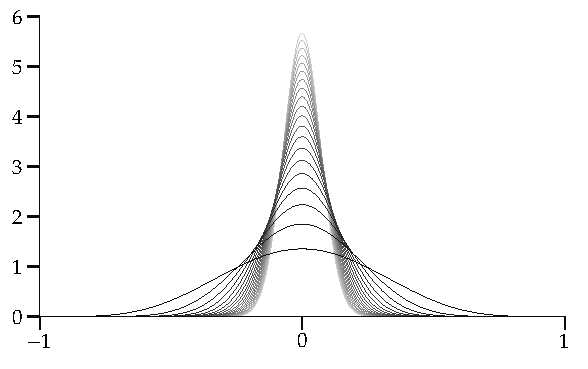
\includegraphics{figures/weierqn}
\caption{Plot of the approximate delta functions $q_n$ on $[-1,1]$ for
$n=5,10,15,20,\ldots,100$ with higher $n$ in lighter shade.\label{fig:weierqn}}
\end{myfigureht}

The functions $q_n$ are peaks around 0 (ignoring what happens outside
of $[-1,1]$) that get narrower and taller as $n$ increases,
while the area underneath is always 1.
A classic approximation idea
is to do a \emph{\myindex{convolution}} integral with peaks like this:
For
for $x \in [0,1]$, let
\begin{equation*}
p_n(x) \coloneqq \int_{0}^1 g(t)q_n(x-t) \,dt \quad \left( = \int_{-\infty}^\infty
g(t)q_n(x-t) \,dt \right) .
\end{equation*}
The idea of this convolution is that we do a \myquote{weighted average} of the
function $g$ around the point $x$ using $q_n$ as the weight.
See \figureref{fig:approxdeltaconv}.

\begin{myfigureht}
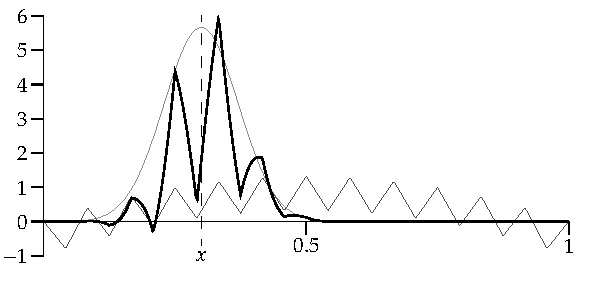
\includegraphics{figures/approxdeltaconv}
\caption{For $x=0.3$, the plot of $q_{100}(x-t)$ (light gray peak centered
at $x$), some continuous function
$g(t)$ (the jagged line) and the product $g(t)q_{100}(x-t)$ (the bold line).\label{fig:approxdeltaconv}}
\end{myfigureht}

As $q_n$ is a narrow peak, the integral
mostly sees the values of $g$ that are
close to $x$ and it does the weighted average of them.
When the peak gets narrower, we compute this average closer to $x$
and we expect the result to get closer to the value of $g(x)$.  Really, we are
approximating what is called a delta function\footnote{The delta function
is not actually a function,
it is a \myquote{thing} that should give
\myquote{$\int_{-\infty}^\infty g(t) \delta(x-t) \, dt = g(x)$.}}
(don't worry if you have not
heard of this concept),
and functions like $q_n$ are often called
\emph{approximate delta functions}\index{approximate delta function}.
We could do this with any set of polynomials that look like narrower
and narrower peaks near zero.  These just happen to be the simplest ones.
We only need this behavior on $[-1,1]$ as the convolution sees nothing
further than this as $g$ is zero outside $[0,1]$.

Because $q_n$ is a polynomial, we write
\begin{equation*}
q_n(x-t) = a_0(t) + a_1(t)\,x + \cdots + a_{2n}(t)\, x^{2n} ,
\end{equation*}
where $a_k(t)$ are polynomials in $t$, and hence
integrable functions.
So
\begin{equation*}
\begin{split}
p_n(x) & =
\int_{0}^1 g(t)q_n(x-t) \,dt
\\
&=
\left(
\int_0^1
g(t)
a_0(t)\,dt
\right)
+
\left(
\int_0^1
g(t)
a_1(t)\,dt
\right)
\,
x
+
\cdots
+
\left(
\int_0^1
g(t)
a_{2n}(t)\,dt
\right)
\,
x^{2n} .
\end{split}
\end{equation*}
In other words, $p_n$ is a polynomial%
\footnote{%
Do note that the functions $a_j$ depend on $n$, so the coefficients of $p_n$
change as $n$ changes.}
 in $x$.
If $g(t)$ is real-valued, then the functions $g(t)a_j(t)$ are
real-valued and $p_n$ has real coefficients,
proving the \myquote{furthermore} part of the theorem.

We still need to prove that $\{ p_n \}_{n=1}^\infty$ converges to $g$.
We start with estimating the size of $c_n$.
For $x \in [0,1]$, we have that $1-x \leq 1-x^2$.  We estimate
\begin{equation*}
\begin{split}
c_n^{-1}   = \int_{-1}^1 {(1-x^2)}^n \, dx
& = 2\int_0^1 {(1-x^2)}^n \, dx \\
& \geq 2\int_0^{1} {(1-x)}^n \, dx
= \frac{2}{n+1} .
\end{split}
\end{equation*}
So $c_n \leq \frac{n+1}{2} \leq n$.
Let us see how small $q_n$ is if we ignore some small interval around the origin,
where the peak is.
Given any $\delta > 0$, $\delta < 1$,
we have that for all
$x$ such that $\delta \leq \sabs{x} \leq 1$,
\begin{equation*}
q_n(x) \leq c_n {(1-\delta^2)}^n \leq  n{(1-\delta^2)}^n ,
\end{equation*}
because $q_n$ is increasing on $[-1,0]$ and decreasing on $[0,1]$.
By the ratio test, 
$n{(1-\delta^2)}^n$ goes to 0 as $n$ goes to infinity.

The function $q_n$ is even, $q_n(t) = q_n(-t)$, and $g$
is zero outside of $[0,1]$.
So for $x \in [0,1]$,
\begin{equation*}
p_n(x) = 
\int_{0}^1 g(t)q_n(x-t) \, dt
=
\int_{-x}^{1-x} g(x+t)q_n(-t) \, dt
=
\int_{-1}^{1} g(x+t)q_n(t) \, dt .
\end{equation*}
Let $\epsilon > 0$ be given.
As $[-1,2]$ is compact and $g$ is continuous on $[-1,2]$, we have that $g$ is uniformly continuous.
Pick $0 < \delta < 1$ such that if
$\sabs{x-y} < \delta$ (and $x,y \in [-1,2]$), then
\begin{equation*}
\sabs{g(x)-g(y)} < \frac{\epsilon}{2} .
\end{equation*}
Let $M$ be such that $\sabs{g(x)} \leq M$ for all $x$.  Let $N$ be
such that for all $n \geq N$,
\begin{equation*}
4M n{(1-\delta^2)}^n < \frac{\epsilon}{2} .
\end{equation*}
Note that 
$\int_{-1}^1 q_n(t) \, dt = 1$ and $q_n(t) \geq 0$ on $[-1,1]$.  So for $n
\geq N$ and every $x \in [0,1]$,
\begin{align*}
\sabs{p_n(x)-g(x)} & =
\abs{\int_{-1}^1 g(x+t)q_n(t) \, dt
-g(x)\int_{-1}^1 q_n(t) \, dt} \\
& =
\abs{\int_{-1}^1 \bigl(g(x+t)-g(x)\bigr)q_n(t) \, dt}
\displaybreak[0]\\
& \leq
\int_{-1}^1 \sabs{g(x+t)-g(x)} q_n(t) \, dt
\displaybreak[0]\\
& =
\int_{-1}^{-\delta} \sabs{g(x+t)-g(x)} q_n(t) \, dt
\quad +
\int_{-\delta}^{\delta} \sabs{g(x+t)-g(x)} q_n(t) \, dt
\\
& \phantom{\leq} +
\int_{\delta}^1 \sabs{g(x+t)-g(x)} q_n(t) \, dt \\
& \leq
2M
\int_{-1}^{-\delta} q_n(t) \, dt
\quad
+
\quad
\frac{\epsilon}{2}
\int_{-\delta}^{\delta} q_n(t) \, dt
\quad
+
\quad
2M
\int_{\delta}^1 q_n(t) \, dt \\
& \leq
2M n{(1-\delta^2)}^n(1-\delta)
\quad
+
\quad
\frac{\epsilon}{2}
\quad
+
\quad
2M n{(1-\delta^2)}^n(1-\delta) \\
& <
4M n{(1-\delta^2)}^n
+
\frac{\epsilon}{2}
< \epsilon . \qedhere
\end{align*}
\end{proof}

A convolution often inherits some property of the functions we are convolving.
In our case the convolution $p_n$ inherited the property of being a
polynomial from $q_n$.  The same idea of the proof is often used 
to get other properties.  If $q_n$ or $g$ is infinitely differentiable, so is $p_n$.
If $q_n$ or $g$ is a solution to a linear differential equation, so is $p_n$.
Etc.

Let us note an immediate application of the Weierstrass theorem.  We have
already seen that countable dense subsets can be very useful.

\begin{cor}
The metric spaces $C\bigl([a,b],\R\bigr)$ and $C\bigl([a,b],\C\bigr)$ each contain a countable dense subset.
\end{cor}

\begin{proof}
Without loss of generality, consider only
$C\bigl([a,b],\R\bigr)$
(why?).
Real polynomials are dense in $C\bigl([a,b],\R\bigr)$ by Weierstrass.
If we show that
every real polynomial can be approximated by polynomials with rational
coefficients, we are done.
Indeed, there are only countably many
rational numbers and so there are only countably many polynomials with
rational coefficients (a countable union of countable sets is countable).

Further without loss of generality, suppose $[a,b]=[0,1]$.  Let
\begin{equation*}
p(x) \coloneqq \sum_{k=0}^n a_k\,  x^k
\end{equation*}
be a polynomial of degree $n$ where $a_k \in \R$.  Given $\epsilon > 0$, pick $b_k \in \Q$
such that $\sabs{a_k-b_k} < \frac{\epsilon}{n+1}$.  Then
if we let
\begin{equation*}
q(x) \coloneqq \sum_{k=0}^n b_k \, x^k ,
\end{equation*}
we have
\begin{equation*}
\sabs{p(x)-q(x)}
=
\abs{\sum_{k=0}^n (a_k-b_k) x^k}
\leq
\sum_{k=0}^n \sabs{a_k-b_k} x^k
\leq
\sum_{k=0}^n \sabs{a_k-b_k}
<
\sum_{k=0}^n \frac{\epsilon}{n+1} = \epsilon . \qedhere
\end{equation*}
\end{proof}

\begin{remark}
While we will not prove so, the corollary above implies that
$C\bigl([a,b],\C\bigr)$ has the same cardinality as $\R$, which may be a
bit surprising.  The set of all functions $[a,b] \to \C$ has
cardinality strictly greater than the cardinality of $\R$, it has the
cardinality of the power set of $\R$.  So the
set of continuous functions is a very tiny subset of the set of all
functions.
\end{remark}

\textbf{Warning!}
The fact that every continuous function $f \colon [-1,1] \to \C$ (or any
interval $[a,b]$) can be uniformly
approximated by polynomials
\begin{equation*}
\sum_{k=0}^n a_k\,  x^k
\end{equation*}
does not mean that every continuous $f$ is analytic, that is, equal to a
power series
\begin{equation*}
\sum_{k=0}^\infty c_k\,  x^k .
\end{equation*}
An analytic function is infinitely differentiable,
however,
the function $\sabs{x}$ is continuous and near the origin
approximable by polynomials,
and so provides a counterexample.

The key distinction is that
the polynomials coming from the Weierstrass theorem are not the partial
sums of a power series.  For each one, the coefficients $a_k$ above can be
completely different---they do not need to come from a single sequence
$\{ c_k \}_{k=1}^\infty$.

\subsection{Stone--Weierstrass approximation}

We want to abstract away what is not really
necessary and prove a general version of the Weierstrass theorem.
The polynomials are dense in the space of continuous
functions on a compact interval.  What other kind of families of
functions are also dense?  And if the domain is an
arbitrary metric space, then we no longer have polynomials
to begin with.

The theorem we will prove is the Stone--Weierstrass theorem\footnote{%
Named after the American mathematician
\href{https://en.wikipedia.org/wiki/Marshall_Harvey_Stone}{Marshall Harvey Stone}
(1903--1989), and the German mathematician
\href{https://en.wikipedia.org/wiki/Karl_Weierstrass}{Karl Theodor Wilhelm Weierstrass}
(1815--1897).}.
First,
we need a very
special case of the Weierstrass theorem though.

\begin{cor}
Let $[-a,a]$ be an interval.  Then there is a sequence of real polynomials
$\{ p_n \}_{n=1}^\infty$ that converges uniformly to $\sabs{x}$ on $[-a,a]$ and such that
$p_n(0) = 0$ for all $n$.
\end{cor}

\begin{proof}
As $f(x) \coloneqq \sabs{x}$ is continuous and real-valued
on $[-a,a]$, the Weierstrass theorem gives a sequence of
real polynomials $\{ \widetilde{p}_n \}_{n=1}^\infty$ that converges to $f$
uniformly on $[-a,a]$.
Let
\begin{equation*}
p_n(x) \coloneqq \widetilde{p}_n(x) - \widetilde{p}_n(0) .
\end{equation*}
Obviously $p_n(0) = 0$.

Given $\epsilon > 0$, let $N$ be such that
for $n \geq N$, we have
$\bigl\lvert\widetilde{p}_n(x)-\sabs{x}\big\rvert <
\nicefrac{\epsilon}{2}$ for all $x \in [-a,a]$.
In particular,
$\sabs{\widetilde{p}_n(0)} < \nicefrac{\epsilon}{2}$.
Then for $n \geq N$,
\begin{equation*}
\bigl\lvert p_n(x)-\sabs{x} \bigr\rvert
=
\bigl\lvert \widetilde{p}_n(x) - \widetilde{p}_n(0) - \sabs{x} \bigr\rvert
\leq
\bigl\lvert \widetilde{p}_n(x) - \sabs{x} \bigr\rvert + \sabs{\widetilde{p}_n(0)} < 
\nicefrac{\epsilon}{2} + \nicefrac{\epsilon}{2} = \epsilon . \qedhere
\end{equation*}
\end{proof}

Generalizing the corollary,
we can make the polynomials from the Weierstrass theorem
be equal to our target function at one point, not just for $\sabs{x}$, but
that's the one we will need.

\begin{defn}
\pagebreak[2]
A set $\sA$ of complex-valued functions $f \colon X \to \C$ is said to be an 
\emph{\myindex{algebra}} (sometimes
\emph{\myindex{complex algebra}} or \emph{algebra over $\C$}) if for all $f,
g \in \sA$ and $c \in \C$, we have
\begin{enumerate}[(i)]
\item $f+g \in \sA$.
\item $fg \in \sA$.
\item $cg \in \sA$.
\end{enumerate}
A \emph{\myindex{real algebra}} or an
\emph{algebra over $\R$} is a set of real-valued
functions that satisfies the three properties above for $c \in \R$.
\end{defn}

We are interested in the case when
$X$ is a compact metric space.  Then
$C(X,\C)$ and $C(X,\R)$ are metric spaces.
Given a set $\sA \subset C(X,\C)$, the set of all uniform
limits is the metric space closure $\widebar{\sA}$.
When we talk about closure of an algebra
from now on we mean the closure in $C(X,\C)$
as a metric space.  Same for $C(X,\R)$.

The set $\sP$ of all polynomials is an algebra in
$C\bigl([a,b],\C\bigr)$, and we
have shown that its closure $\widebar{\sP} = C\bigl([a,b],\C\bigr)$.
That is, it is dense.  That is the sort of result that we wish to prove.

We leave the following proposition as an exercise.

\begin{prop} \label{prop:closureofalgebra}
Suppose $X$ is a compact metric space.
If $\sA \subset C(X,\C)$ is an algebra, then the closure $\widebar{\sA}$ is also an algebra.
Similarly for a real algebra in $C(X,\R)$.
\end{prop}

We distill the properties of polynomials that are sufficient
for an approximation theorem.

\begin{defn}
Let $\sA$ be a set of complex-valued functions defined on a set $X$.
\begin{enumerate}[(i)]
\item $\sA$ \emph{\myindex{separates points}}
if for every $x,y \in X$ with $x \not= y$, there is an $f \in \sA$ such that
$f(x) \not= f(y)$.
\item 
$\sA$ \emph{\myindex{vanishes at no point}} if for every $x \in X$
there is an $f \in \sA$ such that $f(x) \not= 0$.
\end{enumerate}
\end{defn}

\begin{example}
Given any $X \subset \R$ (or $X \subset \C$),
the set $\sP$ of polynomials in one variable separates points and vanishes at no point
on $X$.  That is, $1 \in \sP$, so it vanishes at no point.  And for $x,y \in
X$, $x\not= y$, take $f(t) \coloneqq t$.  Then $f(x) = x \not= y = f(y)$.
So $\sP$ separates points.
\end{example}

\begin{example}
The set of functions of the form
\begin{equation*}
f(t) = a_0 + \sum_{n=1}^k a_n \cos(nt)
\end{equation*}
is an algebra,
which follows by the identity $\cos(mt)\cos(nt) = 
\frac{\cos((n+m) t)}{2}+
\frac{\cos((n-m) t)}{2}$.
The algebra vanishes at no point as it contains a constant function.
It does not separate points if the domain is an interval
$[-a,a]$, as $f(-t) = f(t)$ for all~$t$.
It does separate points if the domain is $[0,\pi]$; $\cos(t)$
is one-to-one on $[0,\pi]$.
\end{example}

\begin{example}
The set $\sP$ of real polynomials with no constant term is an algebra that vanishes at the origin.
Clearly, any function in the closure of $\sP$ also vanishes at the origin,
so the closure of $\sP$ cannot be $C\bigl([0,1],\R\bigr)$.

Similarly, the set of constant functions is an algebra that does not
separate points.  Uniform limits of constants are constants, so we also do
not obtain all continuous functions.
\end{example}

It is interesting that these two properties,
\myquote{vanishes at no point} and
\myquote{separates points,} are sufficient to obtain approximation of any
real-valued continuous function.
Before we prove this theorem, we note that such an algebra can interpolate
a finite number of values exactly.  We will state this result
only for two points as that is all that we will require.

\begin{prop} \label{prop:SWinterpolate}
Suppose $\sA$ is an algebra of complex-valued functions on a set $X$ that separates points
and vanishes at no point.  Suppose $x,y$ are distinct points of $X$, and
$c,d \in \C$.  Then there is an $f \in \sA$ such that
\begin{equation*}
f(x) = c, \qquad f(y) = d .
\avoidbreak
\end{equation*}
If $\sA$ is a real algebra, the conclusion holds for $c,d \in \R$.
\end{prop}

\begin{proof}
There must exist an $g,h,k \in \sA$
such that 
$g(x) \not= g(y)$, $h(x) \not= 0$, $k(y) \not= 0$.
Let
\begin{equation*}
\begin{split}
f & \coloneqq 
c
\frac{\bigl(g - g(y)\bigr)h}{\bigl(g(x)-g(y)\bigr)h(x) } + 
d
\frac{\bigl(g - g(x)\bigr)k}{\bigl(g(y)-g(x)\bigr)k(y)}
\\
& =
c
\frac{gh - g(y)h}{g(x)h(x)-g(y)h(x) } + 
d
\frac{gk - g(x)k}{g(y)k(y)-g(x)k(y)} .
\end{split}
\end{equation*}
We are not dividing by zero (clear from the first formula).
Also by the first formula, $f(x) = c$ and $f(y) = d$.
By the second formula, $f \in \sA$ (as $\sA$ is an algebra).
\end{proof}

\begin{thm}[Stone--Weierstrass, real version]
\label{thm:SWreal}%
\index{Stone--Weierstrass!real version}%
Let $X$ be a compact metric space and $\sA$ a real algebra of real-valued
continuous functions on $X$, such that $\sA$ separates points and vanishes at
no point.  Then the closure $\widebar{\sA} = C(X,\R)$.
\end{thm}

The proof is divided into several claims.

\medskip

\noindent
\textbf{Claim 1:} \emph{If $f \in \widebar{\sA}$, then $\sabs{f} \in
\widebar{\sA}$.}

\begin{proof}
The function $f$ is bounded (continuous on a compact set), so there is an $M$
such that $\sabs{f(x)} \leq M$ for all $x \in X$.
Let $\epsilon > 0$ be given.  By the corollary to the Weierstrass theorem,
there exists a real polynomial $c_1 y + c_2 y^2 + \cdots+ c_n y^n$
(vanishing at $y=0$) such that
\begin{equation*}
\abs{\sabs{y} - \sum_{k=1}^N c_k y^k} < \epsilon
\end{equation*}
for all $y \in [-M,M]$.
Because $\widebar{\sA}$ is an algebra and because there is no constant term in the
polynomial,
\begin{equation*}
\sum_{k=1}^N c_k f^k \in \widebar{\sA} .
\end{equation*}
As $\sabs{f(x)} \leq M$, then  for all $x \in X$
\begin{equation*}
\abs{\sabs{f(x)} - \sum_{k=1}^N c_k {\bigl(f(x)\bigr)}^k}
< \epsilon .
\end{equation*}
So $\sabs{f}$ is in the closure of $\widebar{\sA}$, which is itself closed.
In other words, $\sabs{f} \in \widebar{\sA}$.
\end{proof}

\medskip

\noindent
\textbf{Claim 2:} \emph{If $f \in \widebar{\sA}$ and $g \in \widebar{\sA}$, then
$\max(f,g) \in \widebar{\sA}$ and
$\min(f,g) \in \widebar{\sA}$, where
}
\begin{equation*}
\bigl(\max(f,g)\bigr) (x) \coloneqq \max \bigl\{ f(x), g(x) \bigr\} , \qquad
\text{and} \qquad
\bigl(\min(f,g)\bigr) (x) \coloneqq \min \bigl\{ f(x), g(x) \bigr\} .
\end{equation*}

\begin{proof}
Write:
\begin{equation*}
\max(f,g) = \frac{f+g}{2} + \frac{\sabs{f-g}}{2} ,
\qquad\text{and}\qquad
\min(f,g) = \frac{f+g}{2} - \frac{\sabs{f-g}}{2} .
\end{equation*}
As $\widebar{\sA}$ is an algebra we are done.
\end{proof}

By induction, the claim is also true for the minimum or maximum of a finite
collection of functions.

\medskip

\noindent
\textbf{Claim 3:} \emph{Given $f \in C(X,\R)$, $x \in X$, and $\epsilon > 0$,
there exists a $g_x \in \widebar{\sA}$ with $g_x(x) = f(x)$ and
}
\begin{equation*}
g_x(t) > f(t)-\epsilon \qquad \text{for all } t \in X.
\end{equation*}

\begin{proof}
Fix $f$, $x$, and $\epsilon$.
By \propref{prop:SWinterpolate}, for every $y \in X$, find an $h_y \in
\sA$ such that
\begin{equation*}
h_y(x) = f(x), \qquad h_y(y)=f(y) .
\end{equation*}
As $h_y$ and $f$ are continuous, the function $h_y-f$ is continuous,
and the set
\begin{equation*}
U_y \coloneqq
\bigl\{ t \in X : h_y(t) > f(t) -\epsilon \bigr\}
=
{(h_y-f)}^{-1} \bigl( (-\epsilon,\infty) \bigr)
\end{equation*}
is open (it is the inverse image of an open set by a continuous function).
Furthermore $y \in U_y$.  So the sets $U_y$ cover $X$.
The space $X$ is compact,
so there exist finitely many
points $y_1,y_2,\ldots,y_n$ in $X$ such
that
\begin{equation*}
X = \bigcup_{k=1}^n U_{y_k}  .
\end{equation*}
Let 
\begin{equation*}
g_x \coloneqq \max(h_{y_1},h_{y_2},\ldots,h_{y_n}) .
\end{equation*}
By Claim 2, $g_x \in \widebar{\sA}$.  See \figureref{fig:stonegx}.
Moreover,
\begin{equation*}
g_x(t) > f(t) -\epsilon
\end{equation*}
for all $t \in X$, since for every $t$, there is a $y_k$ such that 
$t \in U_{y_k}$, and so 
$h_{y_k}(t) > f(t) -\epsilon$.
Finally, $h_y(x) = f(x)$ for all $y \in X$, so
$g_x(x) = f(x)$.
\end{proof}

\begin{myfigureht}
\subimport*{figures/}{stonegx.pdf_t}
\caption{Construction of $g_x$ out of two $h_{y_1}$ (longer dashes) and
$h_{y_2}$ (shorter dashes).\label{fig:stonegx}}
\end{myfigureht}

What we have now is for each $x$ a function $g_x \in \widebar{\sA}$
that is within $\epsilon$ of $f$ near $x$ (being continuous),
but also $g_x$ is within $\epsilon$ of $f$ from at least one side at
all points.
If we cover $X$ with neighborhoods where $g_x$ is a good approximation,
we can repeat the idea of the argument with a minimum to get
a function that is within $\epsilon$ from both sides.

\medskip
\pagebreak[2]

\noindent
\textbf{Claim 4:} \emph{If $f \in C(X,\R)$ and $\epsilon > 0$ is given, then there
exists an $\varphi \in \widebar{\sA}$ such that}
\begin{equation*}
\sabs{f(x) - \varphi(x)} < \epsilon .
\end{equation*}

\begin{proof}
For every $x \in X$, find the function $g_x$ as in Claim 3.
Let
\begin{equation*}
V_x \coloneqq \bigl\{ t \in X : g_x(t) < f(t) + \epsilon \bigr\}.
\end{equation*}
The sets $V_x$ are open as $g_x$ and $f$ are continuous.
As $g_x(x) = f(x)$, then $x \in V_x$.  So the sets $V_x$ cover $X$.
By compactness of $X$,
there
are finitely many points $x_1,x_2,\ldots,x_n$ such that
\begin{equation*}
X = \bigcup_{k=1}^n V_{x_k} .
\end{equation*}
Let
\begin{equation*}
\varphi \coloneqq \min(g_{x_1},g_{x_2},\ldots,g_{x_n}) .
\end{equation*}
By Claim 2, $\varphi \in \widebar{\sA}$.  Similarly as before (same argument as in
Claim 3), for all $t \in X$,
\begin{equation*}
\varphi(t) < f(t) + \epsilon .
\end{equation*}
Since all the $g_x$ satisfy $g_x(t) > f(t) - \epsilon$ for all $t \in X$,
$\varphi(t) > f(t) - \epsilon$ as well.
Hence, for all $t$,
\begin{equation*}
-\epsilon < \varphi(t) - f(t) < \epsilon ,
\end{equation*}
which is the desired conclusion.
\end{proof}

The proof of the theorem follows from Claim 4.  The claim states that an
arbitrary continuous function is in the closure of $\widebar{\sA}$,
which is already closed.  The theorem is proved.

\begin{example}
The functions of the form
\begin{equation*}
f(t) = \sum_{k=1}^n c_k \, e^{kt},
\end{equation*}
for $c_k \in \R$,
are dense in $C\bigl([a,b],\R\bigr)$.  Such functions are a real
algebra, which follows from $e^{kt} e^{\ell t} = e^{(k+\ell)t}$.  They separate
points as $e^t$ is one-to-one.
As $e^t > 0$ for all $t$, the algebra
does not vanish at any point.
\end{example}

In general, given a set of functions that separates points and does
not vanish at any point, we let these functions
\emph{generate}\index{generate an algebra}
an algebra
by considering all the linear combinations of arbitrary multiples of such
functions.  That is, we consider all real polynomials without constant term
of such functions.  In the example above,
the algebra is generated by $e^t$.  We 
consider polynomials in $e^t$ without constant term.

\begin{example}
We mentioned that the set of all functions of the form
\begin{equation*}
a_0 +
\sum_{n=1}^N a_n \cos(nt)
\end{equation*}
is an algebra.
When considered on $[0,\pi]$, 
it separates points and vanishes nowhere so
\hyperref[thm:SWreal]{Stone--Weierstrass} applies.
As for polynomials, you \emph{do not} want to conclude that every continuous
function on $[0,\pi]$ has a uniformly convergent
Fourier cosine series, that is, that every continuous
function can be written as
\begin{equation*}
a_0 +
\sum_{n=1}^\infty a_n \cos(nt) .
\end{equation*}
That is \emph{not true}!
There exist continuous functions
whose Fourier series does not converge even pointwise
let alone uniformly.  See \sectionref{sec:fourier}.
\end{example}

To obtain Stone--Weierstrass for complex algebras, we must
make an extra assumption.

\begin{defn}
An algebra $\sA$ is \emph{\myindex{self-adjoint}} if for all $f \in \sA$, the function
$\bar{f}$ defined by $\bar{f}(x) \coloneqq \overline{f(x)}$ is in $\sA$, where by the
bar we mean the complex conjugate.
\end{defn}

\begin{thm}[Stone--Weierstrass, complex version]
\label{thm:SWcomplex}%
\index{Stone--Weierstrass!complex version}%
Let $X$ be a compact metric space and $\sA$ an algebra of complex-valued
continuous functions on $X$, such that $\sA$ separates points, vanishes at
no point, and is self-adjoint.  Then the closure $\widebar{\sA} = C(X,\C)$.
\end{thm}

\begin{proof}
Suppose $\sA_\R \subset \sA$ is the set of the real-valued elements of
$\sA$.
For $f \in \sA$, write $f = u+iv$ where $u$ and $v$ are real-valued.
Then
\begin{equation*}
u = \frac{f+\bar{f}}{2}, \qquad
v = \frac{f-\bar{f}}{2i} .
\end{equation*}
So $u, v \in \sA$ as $\sA$ is a self-adjoint algebra, and since they are
real-valued $u, v \in \sA_\R$.

If $x \not= y$, then find an $f \in \sA$ such that $f(x) \not= f(y)$.  If $f
= u+iv$, then it is obvious that either $u(x) \not= u(y)$ or $v(x) \not=
v(y)$.  So $\sA_\R$ separates points.
%
Similarly, for every $x$ find $f \in \sA$ such that $f(x) \not= 0$.  If $f
= u+iv$, then either $u(x) \not= 0$ or $v(x) \not= 0$.
So $\sA_\R$ vanishes at no point.
%
The set $\sA_\R$ is a real algebra, and satisfies the hypotheses of the
\hyperref[thm:SWreal]{real Stone--Weierstrass theorem}.
Given any $f = u+iv \in C(X,\C)$,
we find $g,h \in \sA_\R$ such that
$\sabs{u(t)-g(t)} < \nicefrac{\epsilon}{2}$ and
$\sabs{v(t)-h(t)} < \nicefrac{\epsilon}{2}$ for all $t \in X$.
Next, $g+i h \in \sA$, and
\begin{multline*}
\abs{f(t) - \bigl(g(t)+ih(t)\bigr)} = 
\abs{u(t)+iv(t) - \bigl(g(t)+ih(t)\bigr)} \\
\leq
\sabs{u(t)-g(t)}+\sabs{v(t)-h(t)} < \nicefrac{\epsilon}{2} +
\nicefrac{\epsilon}{2} = \epsilon
\end{multline*}
for all $t \in X$.
So $\widebar{\sA} = C(X,\C)$.
\end{proof}

The self-adjoint requirement is necessary, although it is not so obvious to
see it.  For an example see \exerciseref{exercise:selfadjointSW}.

We give an interesting application.
When working
with functions of two variables, it may be useful to work with functions
of the form $f(x)g(y)$ rather than $F(x,y)$.  For example, they are easier
to integrate.  We have the following.

\begin{example}
Any continuous $F \colon [0,1] \times [0,1] \to \C$ can be
approximated uniformly by functions of the form
\begin{equation*}
\sum_{j=1}^n f_j(x) g_j(y) ,
\end{equation*}
where $f_j \colon [0,1] \to \C$ and $g_j \colon [0,1] \to \C$ are continuous.

Proof:
It is not hard to see that the functions of the above form are a complex
algebra.  It is equally easy to show that they vanish nowhere, separate
points, and the algebra is self-adjoint.  As $[0,1] \times [0,1]$ is
compact,
\hyperref[thm:SWcomplex]{Stone--Weierstrass} obtains the result.
\end{example}

\subsection{Exercises}

\begin{exercise}
Prove \propref{prop:closureofalgebra}.
Hint: If $\{ f_n \}_{n=1}^\infty$ is a sequence in $C(X,\R)$
converging to $f$, then as $f$ is bounded, show
that $f_n$ is uniformly bounded, that is, there exists a
single bound for all $f_n$ (and $f$).
\end{exercise}

\begin{exercise}
Suppose $X \coloneqq \R$ (not compact in particular).
Show that $f(t) \coloneqq e^t$ is not possible to uniformly approximate
by polynomials on $X$.  Hint: Consider $\babs{\frac{e^t}{t^n}}$
as $t \to \infty$.
\end{exercise}

\begin{exercise}
Suppose $f \colon [0,1] \to \C$ is a uniform limit of a sequence of polynomials
of degree at most $d$, then the limit is a polynomial of degree at most $d$.
Conclude that to approximate a function which is not a polynomial, we
need the degree of the approximations to go to infinity.\\
Hint: First prove that if a sequence of polynomials of degree $d$
converges uniformly to the zero function, then 
the coefficients converge to zero.
One way to do this is linear algebra: Consider a polynomial $p$
evaluated at $d+1$ points
to be a linear operator taking the
coefficients of $p$ to the values of $p$
(an operator in $L(\R^{d+1})$).
\end{exercise}

\begin{exercise}
Suppose $f \colon [0,1] \to \R$ is continuous and
$\int_0^1 f(x) x^n \, dx = 0$ for all $n = 0,1,2,\ldots$.
Show that $f(x) = 0$ for all $x \in [0,1]$.
Hint: Approximate by polynomials to show that $\int_0^1 {\bigl( f(x)
\bigr)}^2 \, dx = 0$.
\end{exercise}

\begin{exercise}
Suppose $I \colon C\bigl([0,1],\R\bigr) \to \R$ is 
a linear continuous function such that
$I(x^n) = \frac{1}{n+1}$
for all $n=0,1,2,3,\ldots$.
Prove that $I(f) = \int_0^1 f$ for all $f \in C\bigl([0,1],\R\bigr)$.
\end{exercise}

\begin{exercise}
Let $\sA$ be the collection of real polynomials in $x^2$,
that is, polynomials of the form
$c_0 + c_1 x^2 + c_2 x^4 + \cdots + c_d x^{2d}$.
\begin{enumerate}[a)]
\item
Show that every $f \in C\bigl([0,1],\R\bigr)$ is a uniform limit of
polynomials from $\sA$.
\item
Find an $f \in  C\bigl([-1,1],\R\bigr)$ that is not a
uniform limit of
polynomials from $\sA$.
\item
Which hypothesis of the real Stone--Weierstrass is not satisfied
for the domain $[-1,1]$?
\end{enumerate}
\end{exercise}

\begin{exercise}
\pagebreak[3]
Let $\sabs{z}=1$ define the unit circle $S^1 \subset \C$.
\begin{enumerate}[a)]
\item
Show that functions of the form
\begin{equation*}
\sum_{k=-n}^n c_k\, z^k
\end{equation*}
are dense in $C(S^1,\C)$.  Notice the negative powers.
\item 
Show that functions of the form
\begin{equation*}
c_0
+
\sum_{k=1}^n c_k \, z^k
+
\sum_{k=1}^n c_{-k}\, \bar{z}^k
\end{equation*}
are dense in $C(S^1,\C)$.  These are so-called harmonic polynomials,
and this approximation leads to, for example, the solution of the
steady state heat problem.
\end{enumerate}
Hint: A good way to write the equation for $S^1$ is $z \bar{z} = 1$.
\end{exercise}

\begin{exercise}
Show that for complex numbers $c_j$, the set of functions
of $x$ on $[-\pi,\pi]$
of the form
\begin{equation*}
\sum_{k=-n}^n c_k \, e^{ik x}
\end{equation*}
satisfies the hypotheses of the complex Stone--Weierstrass theorem
and therefore such functions are dense in the $C\bigl([-\pi,\pi],\C\bigr)$.
\end{exercise}

\begin{exercise} \label{exercise:selfadjointSW}
Let $S^1 \subset \C$ be the unit circle, that is the set where
$\sabs{z} = 1$.  Orient this set counterclockwise.
Let $\gamma(t) \coloneqq e^{it}$.
For the one-form $f(z)\,dz$ we write\footnote{%
Alternatively, one could define $dz \coloneqq dx + i \, dy$ and
extend the path integral from \chapterref{path:chapter} to complex-valued
one-forms.}
\begin{equation*}
\int_{S^1} f(z) \,dz \coloneqq \int_0^{2\pi} f(e^{it}) \, i e^{it} \, dt . 
\end{equation*}
\begin{enumerate}[a)]
\item
Prove that for all nonnegative integers $k = 0,1,2,3,\ldots$, we have
$\int_{S^1} z^k \, dz = 0$.
\item
Prove that if
$P(z) = \sum_{k=0}^n c_k z^k$ is a
polynomial in $z$, then
$\int_{S^1} P(z) \, dz = 0$.
\item
Prove
$\int_{S^1} \bar{z} \, dz \not= 0$.
\item
Conclude that polynomials in $z$ (this algebra of functions is
not self-adjoint) are not dense in $C(S^1,\C)$.
\end{enumerate}
\end{exercise}

\begin{exercise}
Let $(X,d)$ be a compact metric space and
suppose $\sA \subset C(X,\R)$ is a real algebra that separates points, but
such that for some $x_0$, $f(x_0) = 0$ for all $f \in \sA$.  Prove that
every function $g \in C(X,\R)$ such that $g(x_0) = 0$ is a uniform limit
of functions from $\sA$.
\end{exercise}

\begin{exercise}
Let $(X,d)$ be a compact metric space and
suppose $\sA \subset C(X,\R)$ is a real algebra.
Suppose that for each $y \in X$ the closure $\widebar{\sA}$
contains the function $\varphi_y(x) \coloneqq d(y,x)$.
Then $\widebar{\sA} = C(X,\R)$.
\end{exercise}

\begin{exercise}
\pagebreak[2]
\leavevmode
\begin{enumerate}[a)]
\item
Suppose $f \colon [a,b] \to \C$ is continuously 
differentiable.  Show that there exists a sequence of polynomials
$\{ p_n \}_{n=1}^\infty$
that converges in the $C^1$ norm to $f$, that is,
$\snorm{f - p_n}_{[a,b]} + \snorm{f'-p_n'}_{[a,b]} \to 0$ as $n \to \infty$.
\item
Suppose $f \colon [a,b] \to \C$ is $k$ times continuously 
differentiable.  Show that there exists a sequence of polynomials
$\{ p_n \}_{n=1}^\infty$
that converges in the $C^k$ norm to $f$, that is,
\begin{equation*}
\sum_{j=0}^k \norm{f^{(j)} - p_n^{(j)}}_{[a,b]} \to 0 \qquad \text{as} \qquad
n \to \infty.
\end{equation*}
\end{enumerate}
\end{exercise}

\begin{exercise}
\pagebreak[2]
\leavevmode
\begin{enumerate}[a)]
\item
Show that an even function $f \colon [-1,1] \to \R$ is a uniform
limit of polynomials with even powers only, that is, polynomials
of the form $a_0 + a_1 x^2 + a_2 x^4 + \cdots + a_k x^{2k}$.
\item
Show that an odd function $f \colon [-1,1] \to \R$ is a uniform
limit of polynomials with odd powers only, that is, polynomials
of the form $b_1 x + b_2 x^3 + b_3 x^5 + \cdots + b_k x^{2k-1}$.
\end{enumerate}
\end{exercise}

%%%%%%%%%%%%%%%%%%%%%%%%%%%%%%%%%%%%%%%%%%%%%%%%%%%%%%%%%%%%%%%%%%%%%%%%%%%%%%

\sectionnewpage
\section{Fourier series}
\label{sec:fourier}

\sectionnotes{3--4 lectures}

Fourier series\footnote{%
Named after the French mathematician
\href{https://en.wikipedia.org/wiki/Joseph_Fourier}{Jean-Baptiste Joseph Fourier}
(1768--1830).} is perhaps the most important (and the most difficult)
of the series that we cover in
this book.  We saw a few examples of it already,
but let us start
at the beginning.

\subsection{Trigonometric polynomials}

A \emph{\myindex{trigonometric polynomial}} is an expression of the form
\begin{equation*}
a_0 + \sum_{n=1}^N \bigl(a_n \cos(nx) + b_n \sin(nx) \bigr),
\end{equation*}
or equivalently, thanks to Euler's formula ($e^{i\theta} = \cos(\theta) + i
\sin(\theta)$):
\begin{equation*}
\sum_{n=-N}^N c_n e^{inx} .
\end{equation*}
The second form is usually more convenient.  If
$z \in \C$ with $\sabs{z}=1,$ we write $z = e^{ix}$, and so
\begin{equation*}
\sum_{n=-N}^N c_n e^{inx} = 
\sum_{n=-N}^N c_n z^n .
\end{equation*}
So a trigonometric polynomial is really a rational function
of the complex variable $z$
(we are allowing negative powers) evaluated on the unit circle.  There is
a wonderful connection between power series (actually Laurent series because
of the negative powers) and
Fourier series because of this observation,
but we will not investigate this further.

\medskip

Another reason why Fourier series are important and come up in so many
applications is that the functions are eigenfunctions%
\footnote{Eigenfunction is like an eigenvector for a matrix, but for a linear
operator on a vector space of functions.} of various
differential operators.  For example,
\begin{equation*}
\frac{d}{dx} \bigl[ e^{ikx} \bigr] = (ik) e^{ikx}, \qquad
\frac{d^2}{dx^2} \bigl[ e^{ikx} \bigr] = (-k^2) e^{ikx} .
\end{equation*}
That is, they are the functions whose derivative is a scalar (the
eigenvalue) times itself.
Just as eigenvalues and eigenvectors are important in studying matrices,
eigenvalues and eigenfunctions are important when studying linear
differential equations.

\medskip

The functions $\cos (nx)$, $\sin (nx)$, and $e^{inx}$ are $2\pi$-periodic
and hence trigonometric
polynomials are also $2\pi$-periodic.
We could rescale $x$ to make the period different, but the theory is the
same, so we stick with the period $2\pi$.
The antiderivative of $e^{inx}$ is $\frac{e^{inx}}{in}$ and
so
\begin{equation*}
\int_{-\pi}^\pi e^{inx} \, dx =
\begin{cases}
2\pi & \text{if } n=0, \\
0    & \text{otherwise.}
\end{cases}
\end{equation*}
Consider
\begin{equation*}
f(x) \coloneqq \sum_{n=-N}^N c_n e^{inx} ,
\end{equation*}
and for $m=-N,\ldots,N$ compute
\begin{equation*}
\frac{1}{2\pi} \int_{-\pi}^\pi
f(x) e^{-imx} \, dx
=
\frac{1}{2\pi} \int_{-\pi}^\pi
\left(\sum_{n=-N}^N c_n e^{i(n-m)x}\right) \, dx
=
\sum_{n=-N}^N
c_n
\frac{1}{2\pi}
\int_{-\pi}^\pi
e^{i(n-m)x}
 \, dx
=
c_m .
\end{equation*}
We just found a way of computing the coefficients $c_m$ using an integral
of $f$.  If $\sabs{m} > N$, the integral is 0, so we might as
well have included enough zero coefficients to make $\sabs{m} \leq N$.

\begin{prop}
A trigonometric polynomial
$f(x) = \sum_{n=-N}^N c_n\, e^{inx}$
is real-valued for real $x$ if
and only if $c_{-m} = \overline{c_m}$ for all $m=-N,\ldots,N$.
\end{prop}

\begin{proof}
If $f(x)$ is real-valued, that is $\overline{f(x)} = f(x)$, then
\begin{equation*}
\overline{c_m}
=
\overline{
\frac{1}{2\pi} \int_{-\pi}^\pi
f(x) e^{-imx} \, dx
}
=
\frac{1}{2\pi} \int_{-\pi}^\pi
\overline{
f(x) e^{-imx} } \, dx
=
\frac{1}{2\pi} \int_{-\pi}^\pi
f(x) e^{imx} \, dx
= c_{-m} .
\end{equation*}
The complex conjugate goes inside the integral because the integral is
done on real and imaginary parts separately.

On the other hand if 
$c_{-m} = \overline{c_m}$, then
\begin{equation*}
\overline{c_{-m}\, e^{-imx}+ c_{m}\, e^{imx}}
=
\overline{c_{-m}}\, e^{imx}+ \overline{c_{m}}\, e^{-imx}
=
c_{m}\, e^{imx}+ c_{-m}\, e^{-imx} ,
\end{equation*}
which is real valued.  Also $c_0 = \overline{c_0}$, so
$c_0$ is real.
By pairing up the terms, we obtain that $f$ has to be real-valued.
\end{proof}

The functions $e^{inx}$ are also linearly independent.

\begin{prop}
If
\begin{equation*}
\sum_{n=-N}^N c_n \, e^{inx} = 0
\end{equation*}
for all $x \in [-\pi,\pi]$, then $c_n = 0$ for all $n$.
\end{prop}

\begin{proof}
The result follows immediately from the integral formula for $c_n$.
\end{proof}

\subsection{Fourier series}

We now take limits.  The series
\begin{equation*}
\sum_{n=-\infty}^\infty c_n \, e^{inx}
\end{equation*}
is called
the \emph{\myindex{Fourier series}} and the numbers $c_n$
the \emph{\myindex{Fourier coefficients}}.  Using
Euler's formula $e^{i\theta} = \cos(\theta) + i \sin (\theta)$,
we could also develop everything with
sines and cosines, that is, as the series
$a_0 + \sum_{n=1}^\infty a_n \cos(nx) + b_n \sin(nx)$.
It is equivalent, but slightly more messy.

Several questions arise.  What functions are expressible as 
Fourier series?  Obviously, they have to be $2\pi$-periodic, but not every
periodic function is expressible with the series.  Furthermore, if we do have
a Fourier series, where does it converge (where and if at all)?  Does it converge
absolutely?  Uniformly?  Also note that the series has two
limits.  When talking about Fourier series convergence, we often
talk about the following limit:
\begin{equation*}
\lim_{N\to\infty} 
\sum_{n=-N}^N c_n e^{inx} .
\end{equation*}
There are other ways we can sum the series that can get convergence in more
situations, but we refrain from discussing those.

\medskip

Conversely, for an integrable function $f \colon [-\pi,\pi] \to
\C$, call the numbers
\begin{equation*}
c_n \coloneqq 
\frac{1}{2\pi} \int_{-\pi}^\pi
f(x) e^{-inx} \, dx
\end{equation*}
its \emph{Fourier coefficients}.  Often these numbers are
written as $\hat{f}(n)$.\footnote{The notation seems similar
to Fourier transform for those readers that have seen it.
The similarity is not just
coincidental, we are taking a type of Fourier transform here.}
We then formally write down a Fourier series.
As you might imagine such a series might not even converge.
We write\glsadd{not:FS}
\begin{equation*}
f(x) \sim
\sum_{n=-\infty}^\infty c_n \, e^{inx} ,
\end{equation*}
although the $\sim$ doesn't imply anything about the two sides being equal
in any way.  It is simply that we created a formal series using the formula
for the coefficients.

A few sections ago, we proved that the Fourier series 
\begin{equation*}
\sum_{n=1}^\infty \frac{\sin(nx)}{n^2}
\end{equation*}
converges uniformly and hence converges to a continuous function.  This 
example and its proof can be extended to a more general criterion.

\begin{prop}
Let $\sum_{n=-\infty}^\infty c_n\, e^{inx}$ be a Fourier series,
and $C$, $\alpha > 1$ constants such that
\begin{equation*}
\sabs{c_n} \leq \frac{C}{\sabs{n}^\alpha}
\qquad \text{for all } n \in \Z \setminus \{ 0 \}.
\avoidbreak
\end{equation*}
Then the series converges (absolutely and uniformly) to a continuous function on $\R$.
\end{prop}

The proof is to apply the Weierstrass $M$-test (\thmref{thm:weiermtest}) and
the $p$-series test, to find that the series converges uniformly and hence
to a continuous function (\corref{cor:metricuniformcontinuous}).
We can also take derivatives.

\begin{prop}
Let $\sum_{n=-\infty}^\infty c_n\, e^{inx}$ be a Fourier series,
and $C$, $\alpha > 2$ constants such that
\begin{equation*}
\sabs{c_n} \leq \frac{C}{\sabs{n}^\alpha}
\qquad \text{for all } n \in \Z \setminus \{ 0 \}.
\avoidbreak
\end{equation*}
Then the series converges to a continuously differentiable function on $\R$.
\end{prop}

The proof is to note that the series converges to a continuous
function by the previous proposition.
In particular, it converges at some point.
Then differentiate the partial sums
\begin{equation*}
\sum_{n=-N}^{N}
i n c_n \,e^{inx}
\end{equation*}
and notice that for all nonzero $n$
\begin{equation*}
\sabs{i n c_n} \leq \frac{C}{\sabs{n}^{\alpha-1}} .
\end{equation*}
The differentiated series converges uniformly by the $M$-test again.  Since
the differentiated series
converges uniformly, we find that the original series
$\sum_{n=-\infty}^\infty c_n\,e^{inx}$
converges 
to a continuously differentiable function, whose derivative is
the differentiated series (see \thmref{thm:dersconvergecomplex}).

We can iterate the same reasoning.
Suppose there is
some $C$ and $\alpha > k+1$ ($k \in \N$) such that
for all nonzero integers $n$,
\begin{equation*}
\sabs{c_n} 
\leq \frac{C}{\sabs{n}^\alpha} .
\end{equation*}
Then 
the Fourier series converges to a $k$-times continuously differentiable
function.  Therefore, the faster the coefficients go to zero, the more
regular the limit is.

\subsection{Orthonormal systems}

Let us abstract away the exponentials, and
study a more general series for a function.
One fundamental property of the exponentials that makes Fourier series work
is that the exponentials are a so-called \emph{orthonormal system}.
Fix an interval $[a,b]$.  We define an
\emph{\myindex{inner product}} for the space of functions.  We restrict our attention
to Riemann integrable functions as we do not have the Lebesgue
integral, which
would be the natural choice.  Let $f$ and~$g$ be complex-valued 
Riemann integrable functions on $[a,b]$ and define the inner product
\glsadd{not:L2innprod}
\begin{equation*}
\langle f , g \rangle \coloneqq
\int_a^b f(x) \overline{g(x)} \, dx .
\end{equation*}
If you have seen Hermitian inner products in linear algebra, this
is precisely such a product.  We must include the conjugate as we are
working with complex numbers.  We then have the \myquote{size} of $f$, that
is, the $L^2$ norm $\snorm{f}_2$, by (defining the square)
\glsadd{not:L2norm}
\begin{equation*}
\snorm{f}_2^2 \coloneqq
\langle f , f \rangle =
\int_a^b \sabs{f(x)}^2 \, dx .
\end{equation*}

\begin{remark}
Note the similarity to finite dimensions.
For $z = (z_1,z_2,\ldots,z_d) \in \C^d$, one defines
\begin{equation*}
\langle z , w \rangle \coloneqq
\sum_{n=1}^d z_n \overline{w_n} .
\end{equation*}
Then the norm is (usually denoted simply by $\snorm{z}$ in $\C^d$
rather than by $\snorm{z}_2$)
\begin{equation*}
\snorm{z}^2 = 
\langle z , z \rangle =
\sum_{n=1}^d \sabs{z_n}^2 .
\end{equation*}
This is just the euclidean distance to the origin in $\C^d$ (same as
$\R^{2d}$).
\end{remark}

%Let us get back to function spaces.
In what follows, we will
assume all functions are Riemann integrable.

\begin{defn}
Let $\{ \varphi_n \}_{n=1}^\infty$ be a sequence of integrable complex-valued
functions on $[a,b]$.  We say that this is an
\emph{\myindex{orthonormal system}} if
\begin{equation*}
\langle \varphi_n , \varphi_m \rangle
=
\int_a^b \varphi_n(x) \, \overline{\varphi_m(x)} \, dx
= 
\begin{cases}
1 & \text{if } n=m, \\
0 & \text{otherwise.}
\end{cases}
\end{equation*}
In particular, $\snorm{\varphi_n}_2 = 1$ for all $n$.  If we
only require that 
$\langle \varphi_n , \varphi_m \rangle = 0$ for $m\not= n$, then
the system would be called an \emph{\myindex{orthogonal system}}.
\end{defn}

We noticed above that
\begin{equation*}
{\left\{ \frac{1}{\sqrt{2\pi}} \, e^{inx} \right\}}_{n=1}^\infty
\end{equation*}
is an orthonormal system.  The factor out in front is to make the norm be 1.

Having an orthonormal system $\{ \varphi_n \}_{n=1}^\infty$ on $[a,b]$ and an integrable function $f$
on $[a,b]$, we can write
a Fourier series relative to $\{ \varphi_n \}_{n=1}^\infty$.  Let
\begin{equation*}
c_n \coloneqq
\langle f , \varphi_n \rangle
=
\int_a^b f(x) \overline{\varphi_n(x)} \, dx ,
\end{equation*}
and write
\begin{equation*}
f(x) \sim \sum_{n=1}^\infty c_n \varphi_n .
\end{equation*}

In other words, the series is
\begin{equation*}
\sum_{n=1}^\infty \langle f , \varphi_n \rangle \varphi_n(x) .
\end{equation*}
Notice the similarity to the expression for the orthogonal
projection of a vector onto a subspace from linear algebra.  We are
in fact doing just that, but in a space of functions.

\begin{thm} \label{thm:l2bestapprox}
Suppose $f$ is a Riemann integrable function on $[a,b]$.
Let $\{ \varphi_n \}_{n=1}^\infty$ be an orthonormal system on $[a,b]$ and
suppose
\begin{equation*}
f(x) \sim \sum_{n=1}^\infty c_n \varphi_n(x) .
\end{equation*}
If
\begin{equation*}
s_k (x) \coloneqq \sum_{n=1}^k c_n \varphi_n(x)
\quad\text{and}\quad
p_k (x) \coloneqq \sum_{n=1}^k d_n \varphi_n(x)
\end{equation*}
for some other sequence $\{ d_n \}_{n=1}^\infty$, then
\begin{equation*}
\int_a^b \sabs{f(x)-s_k(x)}^2 \, dx = \snorm{f-s_k}_2^2 \leq
\snorm{f-p_k}_2^2 = \int_a^b \sabs{f(x)-p_k(x)}^2 \, dx
\end{equation*}
with equality only if $d_n = c_n$ for all $n=1,2,\ldots,k$.
\end{thm}

In other words, the partial sums of the Fourier series are the best approximation with respect to the
$L^2$ norm.

\begin{proof}
Let us write
\begin{equation*}
\int_a^b \sabs{f-p_k}^2
=
\int_a^b \sabs{f}^2
-
\int_a^b f \widebar{p_k}
-
\int_a^b \widebar{f} p_k
+
\int_a^b \sabs{p_k}^2 .
\end{equation*}
Now
\begin{equation*}
\int_a^b f \widebar{p_k}
=
\int_a^b f \sum_{n=1}^k \overline{d_n} \overline{\varphi_n}
=
 \sum_{n=1}^k \overline{d_n} \int_a^b f \, \overline{\varphi_n}
=
 \sum_{n=1}^k \overline{d_n} c_n ,
\end{equation*}
and
\begin{equation*}
\int_a^b \sabs{p_k}^2
=
\int_a^b
\sum_{n=1}^k d_n \varphi_n
\sum_{m=1}^k \overline{d_m} \overline{\varphi_m}
=
\sum_{n=1}^k
\sum_{m=1}^k 
d_n
\overline{d_m} 
\int_a^b
\varphi_n
\overline{\varphi_m}
=
\sum_{n=1}^k
\sabs{d_n}^2 .
\end{equation*}
So
\begin{equation*}
\int_a^b \sabs{f-p_k}^2
=
\int_a^b \sabs{f}^2
-
\sum_{n=1}^k \overline{d_n} c_n
-
\sum_{n=1}^k d_k \overline{c_n}
+
\sum_{n=1}^k
\sabs{d_n}^2
=
\int_a^b \sabs{f}^2
-
\sum_{n=1}^k \sabs{c_n}^2
+
\sum_{n=1}^k
\sabs{d_n-c_n}^2 .
\end{equation*}
This is minimized precisely when $d_n = c_n$.
\end{proof}

When we do plug in $d_n = c_n$, then
\begin{equation*}
\int_a^b \sabs{f-s_k}^2
=
\int_a^b \sabs{f}^2
-
\sum_{n=1}^k \sabs{c_n}^2
\end{equation*}
and so for all $k$,
\begin{equation*}
\sum_{n=1}^k \sabs{c_n}^2
\leq
\int_a^b \sabs{f}^2
\end{equation*}
Note that
\begin{equation*}
\sum_{n=1}^k \sabs{c_n}^2 = \snorm{s_k}_2^2
\end{equation*}
by the calculation above.
We take a limit to obtain the so-called
\emph{\myindex{Bessel's inequality}}.

\begin{thm}[Bessel's inequality\footnote{%
Named after the German astronomer, mathematician, physicist, and geodesist
\href{https://en.wikipedia.org/wiki/Friedrich_Bessel}{Friedrich Wilhelm Bessel}
(1784--1846).}] \label{thm:bessels}
Suppose $f$ is a Riemann integrable function on $[a,b]$.
Let $\{ \varphi_n \}_{n=1}^\infty$ be an orthonormal system on $[a,b]$ and
suppose
\begin{equation*}
f(x) \sim \sum_{n=1}^\infty c_n \varphi_n(x) .
\end{equation*}
Then
\begin{equation*}
\sum_{n=1}^\infty \sabs{c_n}^2
\leq
\int_a^b \sabs{f}^2
= \snorm{f}_2^2 .
\end{equation*}
\end{thm}

In particular, if $\int_a^b \sabs{f}^2 < \infty$, the series
converges and hence
\begin{equation*}
\lim_{k \to \infty} c_k = 0 .
\end{equation*}

\subsection{The Dirichlet kernel and approximate delta functions}

We return to the trigonometric Fourier series.
The system $\{ e^{inx} \}_{n=1}^\infty$ is orthogonal, but not orthonormal if we simply
integrate over $[-\pi,\pi]$.  We can rescale the integral
and hence the inner product to make 
$\{ e^{inx} \}_{n=1}^\infty$ orthonormal.  That is, if we replace
\begin{equation*}
\int_a^b \qquad \text{with} \qquad
\frac{1}{2\pi} \int_{-\pi}^\pi,
\end{equation*}
(we are just rescaling the $dx$ really)\footnote{%
Mathematicians in this field sometimes simplify matters with
a tongue-in-cheek definition that $1=2\pi$.},
then everything works and we obtain that the system
$\{ e^{inx} \}_{n=1}^\infty$
is orthonormal with respect to the inner product
\begin{equation*}
\langle f , g \rangle =
\frac{1}{2\pi} \int_{-\pi}^\pi f(x) \, \overline{g(x)} \, dx .
\end{equation*}

Suppose $f \colon \R \to \C$ is $2\pi$-periodic and integrable
on $[-\pi,\pi]$.
Let
\begin{equation*}
c_n \coloneqq 
\frac{1}{2\pi} \int_{-\pi}^\pi
f(x) e^{-inx} \, dx .
\end{equation*}
Write
\begin{equation*}
f(x) \sim
\sum_{n=-\infty}^\infty c_n \,e^{inx} .
\end{equation*}
Define the \emph{\myindex{symmetric partial sums}}
\glsadd{not:FSsympartsum}
\begin{equation*}
s_N(f;x) \coloneqq 
\sum_{n=-N}^N c_n \,e^{inx} .
\end{equation*}
The inequality leading up to Bessel now reads:
\begin{equation*}
\frac{1}{2\pi} \int_{-\pi}^\pi
\sabs{s_N(f;x)}^2 \, dx =
\sum_{n=-N}^N \sabs{c_n}^2
\leq
\frac{1}{2\pi} \int_{-\pi}^\pi
\sabs{f(x)}^2
\, dx .
\end{equation*}

Let the \emph{\myindex{Dirichlet kernel}} be
\begin{equation*}
D_N(x) \coloneqq \sum_{n=-N}^N e^{inx} .
\end{equation*}
We claim that
\begin{equation*}
D_N(x) =
%\sum_{n=-N}^N e^{inx}
%=
\frac{\sin\bigl( (N+\nicefrac{1}{2})x \bigr)}{\sin(\nicefrac{x}{2})} ,
\end{equation*}
for $x$ such that $\sin(\nicefrac{x}{2}) \not= 0$.  The left-hand
side is continuous on $\R$, and hence the right-hand side extends continuously to
all of $\R$.
To show the claim,
we use a familiar trick:
\begin{equation*}
(e^{ix}-1) D_N(x) = e^{i(N+1)x} - e^{-iNx} .
\end{equation*}
Multiply by $e^{-ix/2}$
\begin{equation*}
(e^{ix/2}-e^{-ix/2}) D_N(x) = e^{i(N+\nicefrac{1}{2})x} -
e^{-i(N+\nicefrac{1}{2})x} .
\end{equation*}
The claim follows.

We expand the definition of $s_N$
\begin{multline*}
s_N(f;x) = 
\sum_{n=-N}^N \frac{1}{2\pi} \int_{-\pi}^\pi f(t) e^{-int}  \,  dt ~ e^{inx}
\\
=
\frac{1}{2\pi} \int_{-\pi}^\pi f(t) \sum_{n=-N}^N e^{in(x-t)} \, dt
=
\frac{1}{2\pi} \int_{-\pi}^\pi f(t) D_N(x-t) \, dt .
\end{multline*}
If you replace $x-t$ with $t-x$ ($D_N$ is even), we see that
convolution strikes again!
As $D_N$ and $f$ are $2\pi$-periodic, we may also change variables and write 
\begin{equation*}
s_N(f;x) = 
\frac{1}{2\pi} \int_{x-\pi}^{x+\pi} f(x-t) D_N(t) \, dt
=
\frac{1}{2\pi} \int_{-\pi}^\pi f(x-t) D_N(t) \, dt .
\end{equation*}
See \figureref{fig:approxdeltas} for a plot of $D_N$ for $N=5$ and $N=20$.

\begin{myfigureht}
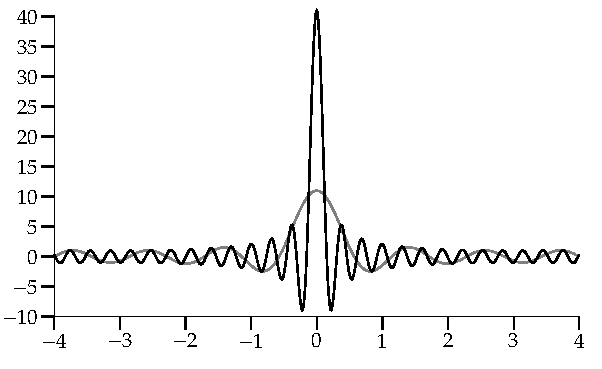
\includegraphics{figures/approxdeltas}
\caption{Plot of $D_N(x)$ for $N=5$ (gray) and $N=20$
(black).\label{fig:approxdeltas}}
\end{myfigureht}

The central peak gets taller and taller as $N$ gets larger,
and the side peaks stay small.
We are convolving (again) with
\emph{approximate delta functions}\index{approximate delta function},
although these functions have
all these oscillations away from zero.  The oscillations on the side do not go away
but they are eventually so fast that we expect the integral to just sort of
cancel itself out there.
Overall, we expect that
$s_N(f)$ goes to $f$.  Things are not always simple,
but under some conditions on $f$, such a conclusion holds.  For this reason
people write
\begin{equation*}
2\pi \, \delta(x) \sim \sum_{n=\infty}^\infty e^{inx} ,
\end{equation*}
where $\delta$ is the \myquote{delta function} (not really a function),
which is an object that will give something like
\myquote{$\int_{-\pi}^{\pi} f(x-t) \delta(t) \, dt = f(x)$.}
We can think of $D_N(x)$ converging in some sense to $2 \pi\, \delta(x)$.
However, we have not defined (and will not define) what the delta function
is, nor what does it mean for it to be a limit of $D_N$ or have a Fourier series.

\subsection{Localization}

If $f$ satisfies a Lipschitz condition at a point, then
the Fourier series converges at that point.

\begin{thm} \label{thm:fourierlocalization}
Let $x$ be fixed and let $f$ be a $2\pi$-periodic function
Riemann integrable on $[-\pi,\pi]$.  Suppose
there exist $\delta > 0$ and $M$ such that
\begin{equation*}
\sabs{f(x+t)-f(x)} \leq M \sabs{t}
\end{equation*}
for all $t \in (-\delta,\delta)$, then
\begin{equation*}
\lim_{N \to \infty} s_N(f;x) = f(x) .
\end{equation*}
\end{thm}

In particular,
if $f$ is continuously
differentiable at $x$,
then we obtain convergence (exercise).
%We state an often-used version of this corollary.
A function $f \colon [a,b] \to \C$ is
\emph{\myindex{continuous piecewise smooth}}\index{piecewise smooth}
if it is continuous and there exist points
$x_0 = a < x_1 < x_2 < \cdots < x_k = b$
such that for every $j$, $f$ restricted to $[x_j,x_{j+1}]$
is continuously differentiable (up to the endpoints).

\begin{cor} \label{cor:fourierpiecewisesmooth}
Let $f$ be a $2\pi$-periodic function
Riemann integrable on $[-\pi,\pi]$.  Suppose
there exist $x\in \R$ and $\delta > 0$ such that $f$ is continuous piecewise
smooth on $[x-\delta,x+\delta]$, then
\begin{equation*}
\lim_{N \to \infty} s_N(f;x) = f(x) .
\end{equation*}
\end{cor}

The proof of the corollary is left as an exercise.  Let us prove the
theorem.

\begin{proof}[Proof of \thmref{thm:fourierlocalization}]
For all $N$,
\begin{equation*}
\frac{1}{2\pi} \int_{-\pi}^\pi D_N = 1 .
\end{equation*}
Write
\begin{equation*}
\begin{split}
s_N(f;x)-f(x) & =
\frac{1}{2\pi} \int_{-\pi}^\pi f(x-t) D_N(t) \, dt 
-
f(x)
\frac{1}{2\pi} \int_{-\pi}^\pi D_N(t) \, dt
\\
& = 
\frac{1}{2\pi} \int_{-\pi}^\pi \bigl( f(x-t) - f(x) \bigr) D_N(t) \, dt 
\\
& = 
\frac{1}{2\pi} \int_{-\pi}^\pi \frac{f(x-t) - f(x)}{\sin(\nicefrac{t}{2})} \sin\bigl(
(N+\nicefrac{1}{2})t \bigr) \, dt .
\end{split}
\end{equation*}
By the hypotheses,
for small nonzero $t$ we get
\begin{equation*}
\abs{ \frac{f(x-t) - f(x)}{\sin(\nicefrac{t}{2})} }
\leq
\frac{M\sabs{t}}{\sabs{\sin(\nicefrac{t}{2})}} .
\end{equation*}
As $\sin(\theta) = \theta + h(\theta)$ where $\frac{h(\theta)}{\theta} \to
0$ as $\theta \to 0$,
we notice that
$\frac{M\sabs{t}}{\sabs{\sin(\nicefrac{t}{2})}}$ is continuous at the origin
and hence 
$\frac{f(x-t) - f(x)}{\sin(\nicefrac{t}{2})}$ must be bounded near the origin.
As $t=0$ is the only place on $[-\pi,\pi]$ where the denominator vanishes,
it is the only place where there could be a problem.  The function is
also Riemann integrable.  We use a trigonometric identity
\begin{equation*}
\sin\bigl( (N+\nicefrac{1}{2})t \bigr)
=
\cos(\nicefrac{t}{2}) \sin(Nt) + 
\sin(\nicefrac{t}{2}) \cos(Nt) ,
\end{equation*}
so
\begin{multline*}
\frac{1}{2\pi} \int_{-\pi}^\pi \frac{f(x-t) - f(x)}{\sin(\nicefrac{t}{2})} \sin\bigl(
(N+\nicefrac{1}{2})t \bigr) \, dt 
= \\
\frac{1}{2\pi} \int_{-\pi}^\pi
\left( \frac{f(x-t) - f(x)}{\sin(\nicefrac{t}{2})}
\cos (\nicefrac{t}{2}) \right) \sin (Nt) \, dt
+
\frac{1}{2\pi} \int_{-\pi}^\pi \bigl( f(x-t) - f(x) \bigr)
\cos (Nt) \, dt .
\end{multline*}
Now 
$\frac{f(x-t) - f(x)}{\sin(\nicefrac{t}{2})} \cos (\nicefrac{t}{2})$
and
$\bigl( f(x-t) - f(x) \bigr)$ are bounded Riemann integrable functions
and so their Fourier coefficients go to zero by \thmref{thm:bessels}.  So the two
integrals on the right-hand side, which compute the Fourier coefficients
for the real version of the Fourier series go to 0 as $N$ goes to infinity.
This is because $\sin(Nt)$ and $\cos(Nt)$ are also orthonormal systems
with respect to the same inner product.
Hence $s_N(f;x)-f(x)$ goes to 0, that is, $s_N(f;x)$ goes to $f(x)$.
\end{proof}

The theorem also says that convergence depends only on local behavior.

\begin{cor}
Suppose $f$ is a $2\pi$-periodic function, Riemann integrable on $[-\pi,\pi]$.
If $J$ is an open interval and $f(x) = 0$ for all $x \in J$,
then $\lim\limits_{N\to\infty} s_N(f;x) = 0$ for all $x \in J$.

In particular, if $f$ and $g$ are $2\pi$-periodic functions,
Riemann integrable on $[-\pi,\pi]$, $J$ an open interval, and $f(x) = g(x)$
for all $x \in J$, then for all $x \in J$,
the sequence
$\bigl\{ s_N(f;x) \bigr\}_{N=1}^\infty$ converges if and only if
$\bigl\{ s_N(g;x) \bigr\}_{N=1}^\infty$ converges.
\end{cor}

The first claim follows by taking $M=0$ in the theorem.
The \myquote{In particular} follows by considering $f-g$, which
is zero on $J$ and $s_N(f-g) = s_N(f) - s_N(g)$.
So convergence at $x$ depends only on the values of the function
near $x$.
However, we saw that the rate of convergence,
that is, how fast does $s_N(f)$
converge to $f$, depends on global behavior of $f$.

Note a subtle difference between the corollary and what 
\hyperref[thm:SWcomplex]{Stone--Weierstrass theorem} gives.
%By Stone--Weierstrass, 
Any continuous function on $[-\pi,\pi]$ can be uniformly approximated
by trigonometric polynomials, but these trigonometric polynomials may
not be the partial sums $s_N$.

\subsection{Parseval's theorem}

Finally,
convergence always happens in the $L^2$ sense and
operations on the (infinite) vectors of
Fourier coefficients are the same as the operations using the integral
inner product.

%\begin{samepage}
\begin{thm}[Parseval\footnote{%
Named after the French mathematician
\href{https://en.wikipedia.org/wiki/Marc-Antoine_Parseval}{Marc-Antoine
Parseval}
(1755--1836).}] \index{Parseval's theorem}
Let $f$ and $g$ be $2\pi$-periodic functions, Riemann integrable 
on $[-\pi,\pi]$
with
\begin{equation*}
f(x) \sim
\sum_{n=-\infty}^\infty c_n \,e^{inx}
\qquad \text{and} \qquad
g(x) \sim
\sum_{n=-\infty}^\infty d_n \,e^{inx} .
\end{equation*}
Then
\begin{equation*}
\lim_{N\to\infty} \snorm{f-s_N(f)}_2^2 = 
\lim_{N\to\infty}
\frac{1}{2\pi}
\int_{-\pi}^\pi
\sabs{f(x)-s_N(f;x)}^2 \, dx
=0 .
\end{equation*}
Also
\begin{equation*}
\langle f , g \rangle =
\frac{1}{2\pi}
\int_{-\pi}^\pi
f(x) \overline{g(x)}\, dx
=
\sum_{n=-\infty}^\infty c_n \overline{d_n} ,
\end{equation*}
and
\begin{equation*}
\snorm{f}_2^2
=
\frac{1}{2\pi}
\int_{-\pi}^\pi
\sabs{f(x)}^2 \, dx
=
\sum_{n=-\infty}^\infty \sabs{c_n}^2.
\end{equation*}
\end{thm}
%\end{samepage}

\begin{proof}
There exists (exercise)
a continuous $2\pi$-periodic function $h$ such that
\begin{equation*}
\snorm{f-h}_2 < \epsilon .
\end{equation*}
Via \hyperref[thm:SWcomplex]{Stone--Weierstrass},
approximate $h$ with a trigonometric polynomial
uniformly.  That is, there is a trigonometric polynomial $P(x)$
such that
$\sabs{h(x) - P(x)} < \epsilon$ for all $x$.
Hence
\begin{equation*}
\snorm{h-P}_2
=
\sqrt{
\frac{1}{2\pi}
\int_{-\pi}^{\pi}
\sabs{h(x)-P(x)}^2
\,
dx
}
\leq \epsilon.
\end{equation*}
If $P$ is of degree $N_0$, then for all $N \geq N_0$
\begin{equation*}
\snorm{h-s_N(h)}_2 \leq \snorm{h-P}_2 \leq \epsilon ,
\end{equation*}
as $s_N(h)$ is the best approximation for $h$ in $L^2$ (\thmref{thm:l2bestapprox}).
By the inequality leading up to Bessel, we have
\begin{equation*}
\snorm{s_N(h)-s_N(f)}_2
=
\snorm{s_N(h-f)}_2
\leq
\snorm{h-f}_2 \leq \epsilon .
\end{equation*}
The $L^2$ norm satisfies the triangle inequality (exercise).
Thus, for all $N \geq N_0$,
\begin{equation*}
\snorm{f-s_N(f)}_2
\leq
\snorm{f-h}_2
+
\snorm{h-s_N(h)}_2
+
\snorm{s_N(h)-s_N(f)}_2
\leq 3\epsilon .
\end{equation*}
Hence, the first claim follows.

Next,
\begin{equation*}
\langle s_N(f) , g \rangle
=
\frac{1}{2\pi}
\int_{-\pi}^\pi
s_N(f;x) \overline{g(x)} \, dx
=
\sum_{k=-N}^N
c_k 
\frac{1}{2\pi}
\int_{-\pi}^\pi
e^{ikx}
\overline{g(x)} \, dx
=
\sum_{k=-N}^N
c_k 
\overline{d_k} .
\end{equation*}
We need the Schwarz (or Cauchy--Schwarz or Cauchy--Bunyakovsky--Schwarz)
inequality, that is,
\begin{equation*}
{\abs{\int_a^b f\bar{g}}}^2
\leq
\left( \int_a^b \sabs{f}^2 \right)
\left( \int_a^b \sabs{g}^2 \right) .
\end{equation*}
This is left as an exercise.  The proof is not really
different from the finite-dimensional version.
So
\begin{equation*}
\begin{split}
\abs{\int_{-\pi}^\pi f\bar{g} - \int_{-\pi}^\pi s_N(f)\bar{g}}
& =
\abs{\int_{-\pi}^\pi (f- s_N(f))\bar{g}} \\
%& \leq
%\int_{-\pi}^\pi \sabs{f- s_N(f)}\, \sabs{g} \\
& \leq
{\left(\int_{-\pi}^\pi \sabs{f- s_N(f)}^2 \right)}^{1/2}
{\left( \int_{-\pi}^\pi \sabs{g}^2 \right)}^{1/2} .
\end{split}
\end{equation*}
The right-hand side goes to 0 as $N$ goes to infinity by the first
claim of the theorem.
That is, as $N$ goes to infinity, $\langle s_N(f),g \rangle$
goes to $\langle f,g \rangle$, and
the second claim is proved.  The last claim in the theorem follows by using
$g=f$.
\end{proof}

\subsection{Exercises}

\begin{exercise}
Consider the Fourier series
\begin{equation*}
\sum_{n=1}^\infty \frac{1}{2^n} \sin(2^n x) .
\end{equation*}
Show that the series converges uniformly and absolutely to a continuous
function.  Note: This is another example of a nowhere differentiable
function (you do not have to prove that)\footnote{%
See
G.\ H.\ Hardy, \emph{Weierstrass's Non-Differentiable Function},
Transactions of the American Mathematical Society,
\textbf{17}, No.\ 3 (Jul., 1916), pp.\ 301--325.}.
See \figureref{fig:fourierserweier}.
\begin{myfigureht}
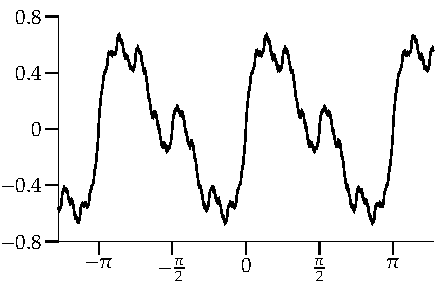
\includegraphics{figures/fourierserweier}
\caption{Plot of 
$\sum_{n=1}^\infty \frac{1}{2^n} \sin(2^n x)$.\label{fig:fourierserweier}}
\end{myfigureht}
\end{exercise}

\begin{exercise}
Suppose that a $2\pi$-periodic function that is Riemann integrable
on $[-\pi,\pi]$, and such that $f$ is continuously differentiable
on some open interval $(a,b)$.  Prove that
for every $x \in (a,b)$, we have $\lim\limits_{N\to\infty} s_N(f;x) = f(x)$.
\end{exercise}

\begin{exercise}
Prove \corref{cor:fourierpiecewisesmooth}, that is,
suppose a $2\pi$-periodic function is continuous piecewise
smooth near a point $x$, then $\lim\limits_{N\to\infty} s_N(f;x) = f(x)$.  Hint: See the previous
exercise.
\end{exercise}

\begin{exercise}
Given a $2\pi$-periodic function $f \colon \R \to \C$ Riemann integrable on
$[-\pi,\pi]$,
and $\epsilon > 0$.
Show that there exists a continuous $2\pi$-periodic function $g \colon \R
\to \C$ such that $\snorm{f-g}_2 < \epsilon$.
\end{exercise}

\begin{exercise}
Prove the Cauchy--Bunyakovsky--Schwarz inequality
for Riemann integrable functions:
\begin{equation*}
{\abs{\int_a^b f\bar{g}}}^2
\leq
\left( \int_a^b \sabs{f}^2 \right)
\left( \int_a^b \sabs{g}^2 \right) .
\end{equation*}
\end{exercise}

\begin{exercise}
Prove the $L^2$ triangle inequality 
for Riemann integrable functions on $[-\pi,\pi]$:
\begin{equation*}
\snorm{f+g}_2 \leq \snorm{f}_2 + \snorm{g}_2 .
\end{equation*}
\end{exercise}

\begin{exercise}
\pagebreak[3]
Suppose for some $C$ and $\alpha > 1$, we have
a real sequence $\{ a_n \}_{n=1}^\infty$ with
$\abs{a_n} \leq \frac{C}{n^\alpha}$ for all $n$.
Let
\begin{equation*}
g(x) \coloneqq \sum_{n=1}^\infty a_n \sin(n x) .
\end{equation*}
\begin{enumerate}[a)]
\item
Show that $g$ is continuous.
\item
Formally (that is, suppose you can differentiate under the sum)
find a solution (formal solution, that is, do not yet worry about convergence)
to the differential equation
\begin{equation*}
y''+ 2 y = g(x)
\end{equation*}
of the form
\begin{equation*}
y(x) = \sum_{n=1}^\infty b_n \sin(n x) .
\end{equation*}
\item
Then show that this solution $y$ is twice continuously differentiable,
and in fact solves the equation.
\end{enumerate}
\end{exercise}

\begin{exercise}
Let $f$ be a $2\pi$-periodic  function such
that $f(x) = x$ for $0 < x < 2\pi$.
Use Parseval's theorem to find
\begin{equation*}
\sum_{n=1}^\infty \frac{1}{n^2} = \frac{\pi^2}{6} .
\end{equation*}
\end{exercise}

\begin{exercise}
Suppose that $c_n = 0$ for all $n < 0$ and $\sum_{n=0}^\infty \sabs{c_n}$
converges.  Let $\D \coloneqq B(0,1) \subset \C$ be the unit disc,
and $\overline{\D} = C(0,1)$ be the closed unit disc.
Show that there exists a continuous function
$f \colon \overline{\D} \to \C$ that is analytic on $\D$
and such that on the boundary of $\D$ we have
$f(e^{i\theta}) = \sum_{n=0}^\infty c_n e^{i\theta}$.\\
Hint: If $z=re^{i\theta}$, then $z^n = r^n e^{in\theta}$.
\end{exercise}

\begin{exercise}
Show that
\begin{equation*}
\sum_{n=1}^\infty e^{-1/n} \sin(n x)
\end{equation*}
converges to an infinitely differentiable function.
\end{exercise}

\begin{exercise}
Let $f$ be a $2\pi$-periodic function
such that $f(x) = f(0) + \int_0^x g$
for a function $g$ that is Riemann integrable on every interval.
Suppose
\begin{equation*}
f(x) \sim
\sum_{n=-\infty}^\infty c_n \,e^{inx} .
\end{equation*}
Show that there exists a $C > 0$ such that
$\sabs{c_n} \leq \frac{C}{\sabs{n}}$.
\end{exercise}

\begin{exercise}
\leavevmode
\begin{enumerate}[a)]
\item
Let $\varphi$ be the $2\pi$-periodic function 
defined by $\varphi(x) \coloneqq 0$ if $x \in (-\pi,0)$,
and $\varphi(x) \coloneqq 1$ if $x \in (0,\pi)$,
letting $\varphi(0)$ and $\varphi(\pi)$ be arbitrary.  Show
that $\lim\limits_{N \to \infty} s_N(\varphi;0) = \nicefrac{1}{2}$.
\item
Let $f$ be a $2\pi$-periodic function
Riemann integrable on $[-\pi,\pi]$, 
$x \in \R$, $\delta > 0$, and
there are continuously differentiable
$g \colon [x-\delta,x] \to \C$
and $h \colon [x,x+\delta] \to \C$
where $f(t) = g(t)$ for all $t \in [x-\delta,x)$
and
where $f(t) = h(t)$ for all $t \in (x,x+\delta]$.
Then
$\lim\limits_{N\to\infty} s_N(f;x) = \frac{g(x)+h(x)}{2}$, or in other words,
\begin{equation*}
\lim_{N \to \infty} s_N(f;x) =
\frac{1}{2}
\left(
\lim_{t \to x^-} f(t) +
\lim_{t \to x^+} f(t)
\right) .
\end{equation*}
\end{enumerate}
\end{exercise}
